\documentclass{beamer}
\usepackage{graphicx}
\usepackage{amsmath, esint}

\usepackage{ragged2e}
\usepackage{tikz}
\usetikzlibrary{arrows,shapes}

\usepackage{listings}
\lstset{escapeinside={@(}{)@}}
\usepackage{algorithm}
\usepackage{algorithmic}

\usepackage{tabularx}
\newcolumntype{Y}{>{\centering\arraybackslash}X}

% \usepackage{minted}
\usepackage{xcolor} 
\definecolor{LightGray}{gray}{0.975}

\usepackage{amssymb}

\def\ojoin{\setbox0=\hbox{$\bowtie$}%
  \rule[-.02ex]{.25em}{.4pt}\llap{\rule[\ht0]{.25em}{.4pt}}}
\def\leftouterjoin{\mathbin{\ojoin\mkern-5.8mu\bowtie}}
\def\rightouterjoin{\mathbin{\bowtie\mkern-5.8mu\ojoin}}
\def\fullouterjoin{\mathbin{\ojoin\mkern-5.8mu\bowtie\mkern-5.8mu\ojoin}}

%\usetheme{Warsaw}
\usefonttheme{serif} 

\title[Chapter 6]{Database System Concepts, $7^{th}$ Edition \\ Chapter 6: Database Design Using the E-R Model}
\author{Silberschatz, Korth and Sudarshan}
\date{\today}

\setbeamertemplate{navigation symbols}{}%remove navigation symbols

\defbeamertemplate*{footline}{shadow theme}
{%
  \leavevmode%
  \hbox{\begin{beamercolorbox}[wd=.5\paperwidth,ht=2.5ex,dp=1.125ex,leftskip=.3cm plus1fil,rightskip=.3cm]{author in head/foot}%
    \usebeamerfont{author in head/foot} Database System Concepts \hfill \insertshorttitle
  \end{beamercolorbox}%
  \begin{beamercolorbox}[wd=.5\paperwidth,ht=2.5ex,dp=1.125ex,leftskip=.3cm,rightskip=.3cm plus1fil]{title in head/foot}%
    \usebeamerfont{title in head/foot} \hfill \insertframenumber\,/\,\inserttotalframenumber%
  \end{beamercolorbox}}%
  \vskip0pt%
}

\AtBeginSection[]
{
     \begin{frame}<beamer>
     \frametitle{Plan}
     \tableofcontents[currentsection]
     \end{frame}
}

\newcommand{\toRight}[1]{
    \begin{FlushRight}
        {\tiny #1}
    \end{FlushRight}
} % Align to right

\begin{document}

\frame{\titlepage}

\begin{frame}{Database System Concepts}
    \centering
    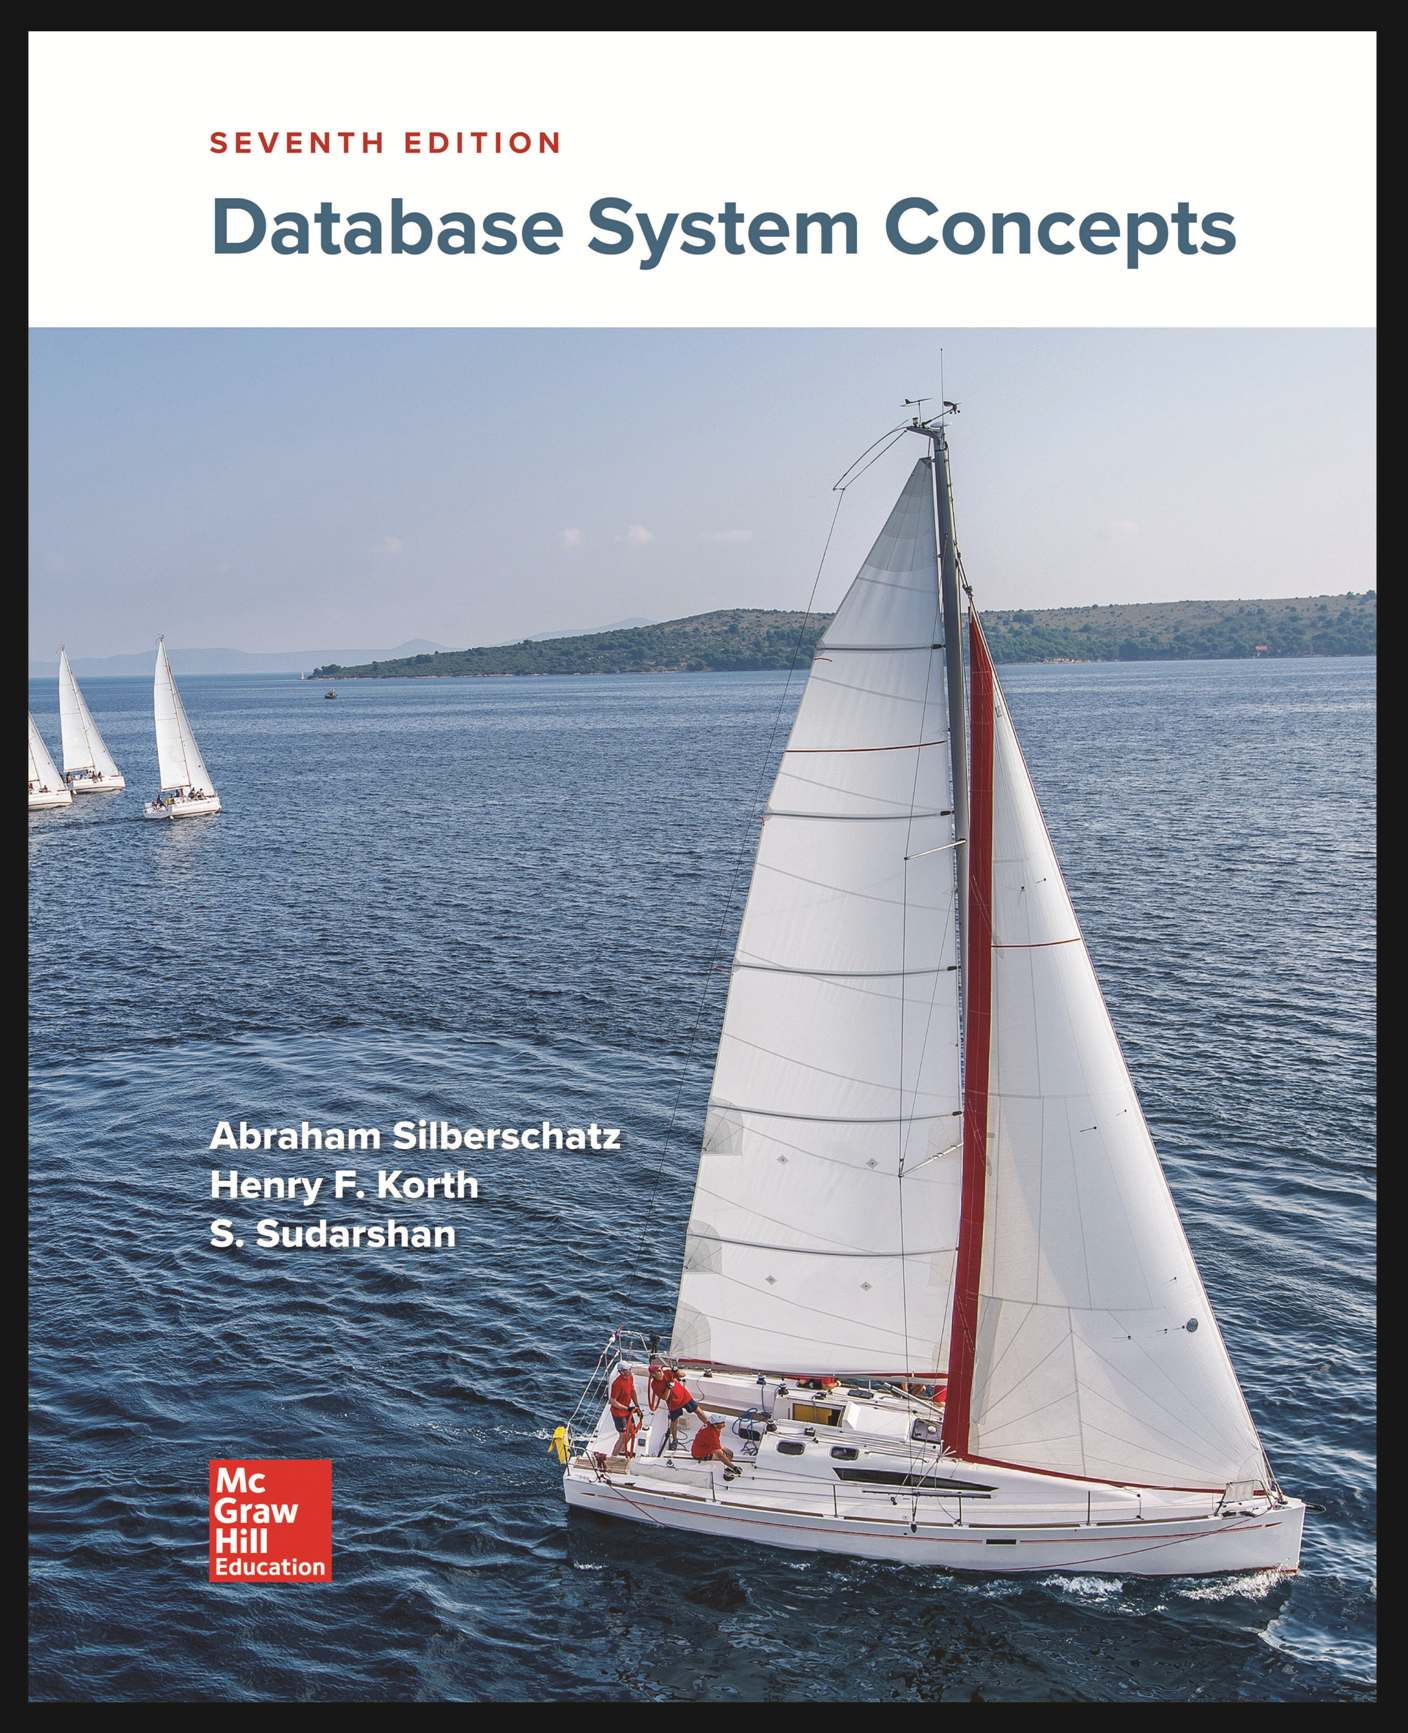
\includegraphics[width=0.5\textwidth]{figures/book_cover.jpg} \\
    \vspace{5mm}
    {
        \tiny
        Content has been extracted from \textit{Database System Concepts}, Seventh Edition, by Silberschatz, Korth and Sudarshan. Mc Graw Hill Education. 2019.\\
        Visit \url{https://db-book.com/}.\\
    }
\end{frame}

\section{Overview of the Design Process}

\begin{frame}{Design Phases}
    \begin{itemize}
        \item Initial phase --characterize fully the data needs of the prospective database users.
        \item Second phase --choosing a data model:
        \begin{itemize}
            \item Applying the concepts of the chosen data model.
            \item Translating these requirements into a conceptual schema of the database.
            \item A fully developed conceptual schema indicates the functional requirements of the enterprise.
            \begin{itemize}
                \item Describe the kinds of operations (or transactions) that will be performed on the data.
            \end{itemize}
        \end{itemize}
    \end{itemize}
\end{frame}

\begin{frame}{Design Phases (Cont.)}
    \begin{itemize}
        \item Final phase --Moving from an abstract data model to the implementation of the database.
        \begin{itemize}
            \item Logical Design --Deciding on the database schema.
            \begin{itemize}
                \item Database design: requires that we find a ``good'' collection of relation schemas.
                \item Business decisions: What attributes should we record in the database?
                \item Computer Science decision: What relation schemas should we have and how should the attributes be distributed among the various relation schemas?
            \end{itemize}
            \item Physical Design --Deciding on the physical layout of the database
        \end{itemize}
    \end{itemize}
\end{frame}

\begin{frame}{Design Alternatives}
    \begin{itemize}
        \item In designing a database schema, we must ensure that we avoid two major pitfalls:
        \begin{itemize}
            \item Redundancy: a bad design may result in repeat information.
            \begin{itemize}
                \item Redundant representation of information may lead to data inconsistency among the various copies of information
            \end{itemize}
            \item Incompleteness: a bad design may make certain aspects of the enterprise difficult or impossible to model.
        \end{itemize}
        \item Avoiding bad designs is not enough. There may be a large number of good designs from which we must choose.
    \end{itemize}
\end{frame}

\begin{frame}{Design Approaches}
    \begin{itemize}
        \item Entity Relationship Model (covered in this chapter).
        \begin{itemize}
            \item Models an enterprise as a collection of entities and relationships.
            \begin{itemize}
                \item Entity: a ``thing'' or ``object'' in the enterprise that is distinguishable from other objects described by a set of attributes.
                \item Relationship: an association among several entities.
            \end{itemize}
            \item Represented diagrammatically by an entity-relationship diagram.
        \end{itemize}
        \item Normalization Theory (Chapter 7).
    \end{itemize}
\end{frame}

\section{The Entity-Relationship Model}

\begin{frame}{Entity Sets}
    \begin{itemize}
        \item An entity is an object that exists and is distinguishable from other objects.
        \begin{itemize}
            \item Example: specific person, company, event, plant...
        \end{itemize}
        \item An entity set is a set of entities of the same type that share the same properties.
        \begin{itemize}
            \item Example: set of all persons, companies, trees, holidays...
        \end{itemize}
        \item An entity is represented by a set of attributes; i.e., descriptive properties possessed by all members of an entity set.
        \begin{itemize}
            \item Example: \\
            \begin{tabular}{r l}
                instructor = & (ID, name, salary ) \\
                    course = & (course\_id, title, credits)\\
            \end{tabular}
        \end{itemize}
        \item A subset of the attributes form a primary key of the entity set; i.e., uniquely identifying each member of the set.
    \end{itemize}
\end{frame}

\begin{frame}{Representing Entity sets in ER Diagram}
    \begin{itemize}
        \item Entity sets can be represented graphically as follows:
        \begin{itemize}
            \item Rectangles represent entity sets.
            \item Attributes listed inside entity rectangle.
            \item Underline indicates primary key attributes.
        \end{itemize}
    \end{itemize}
    \centering
    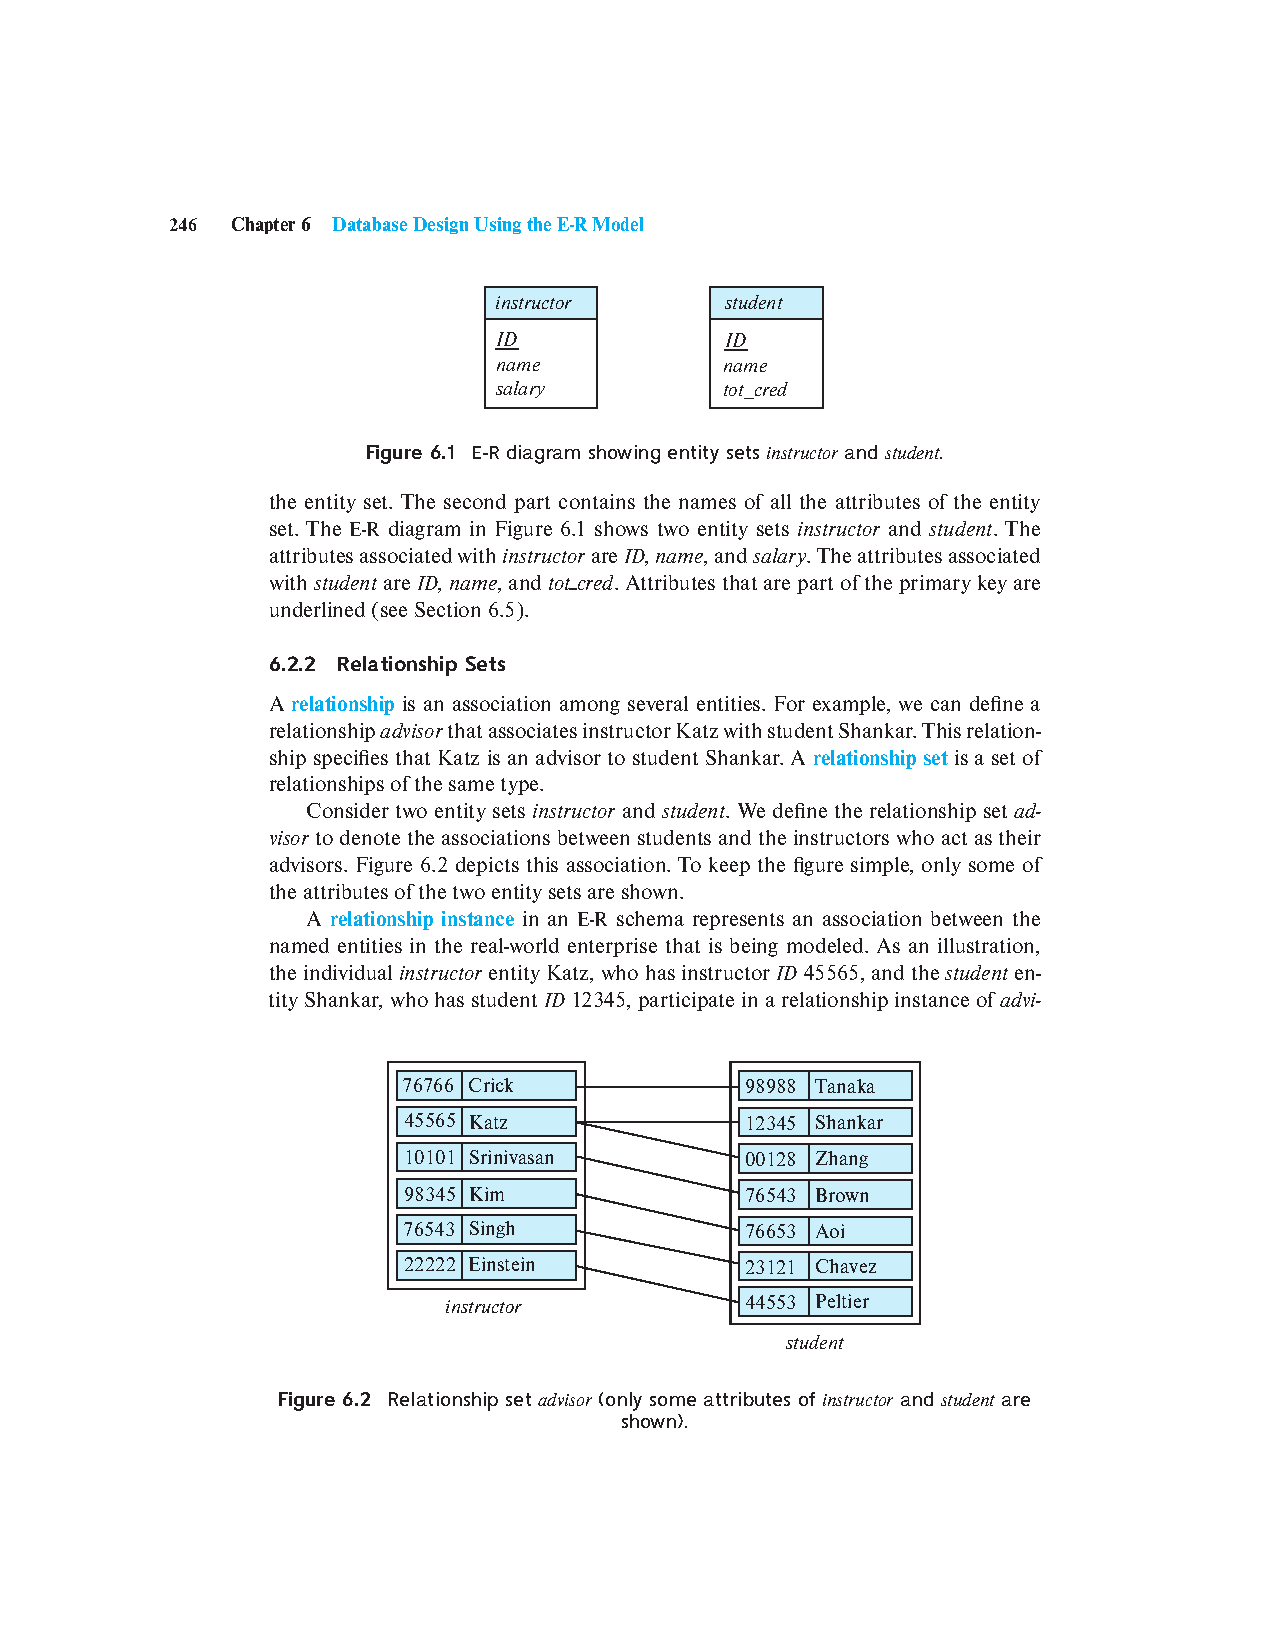
\includegraphics[trim={8.20cm 21cm 7.65cm 4cm}, clip, width=0.65\textwidth]{figures/p246}
\end{frame}

\begin{frame}{Relationship Sets}
    \begin{itemize}
        \item A \textbf{relationship} is an association among several entities.  For example:
        \begin{tabular}{l l l}
            44553 (Peltier) & advisor          & 22222 (Einstein) \\
            student entity  & relationship set & instructor entity \\
        \end{tabular}
        \item A \textbf{relationship set} is a mathematical relation among $n \geq 2$ entities, each taken from entity sets.
        $$
            \{(e_1, e_2, \ldots, e_n)| e_1 \in E_1, e_2 \in E_2, \ldots, e_n \in E_n\}
        $$
        where $(e_1, e_2, \ldots, e_n)$ is a relationship.
        \begin{itemize}
            \item Example: (44553,22222) $\in$ advisor
        \end{itemize}
    \end{itemize}
\end{frame}

\begin{frame}{Relationship Sets (Cont.)}
    \begin{exampleblock}{Example}
        We define the relationship set advisor to denote the associations between students and the instructors who act as their advisors.
    \end{exampleblock}
    \begin{itemize}
        \item Pictorially, we draw a line between related entities.
    \end{itemize}
    \centering
    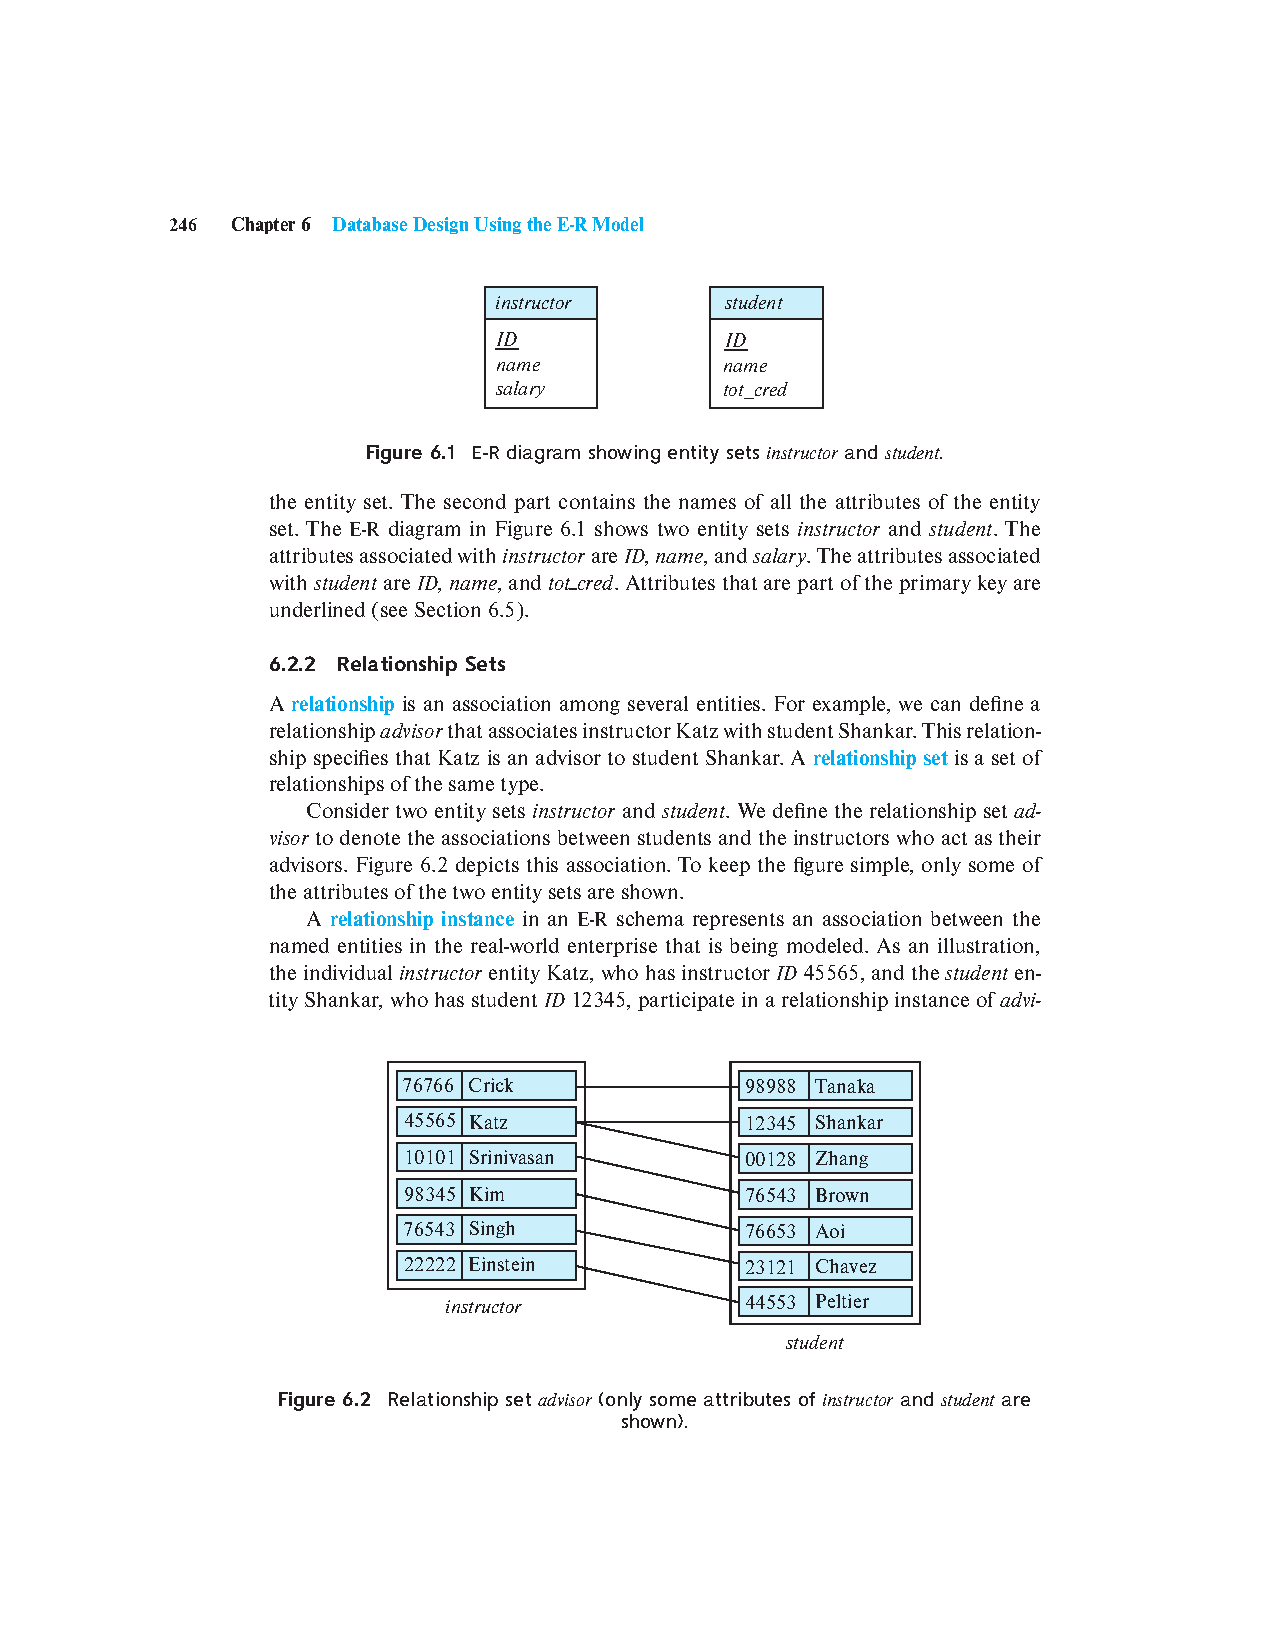
\includegraphics[trim={6.50cm 5cm 6.00cm 17.50cm}, clip, width=0.7\textwidth]{figures/p246}
\end{frame}

\begin{frame}{Representing Relationship Sets via ER Diagrams}
    \begin{itemize}
        \item Diamonds represent relationship sets.
    \end{itemize}
    \centering
    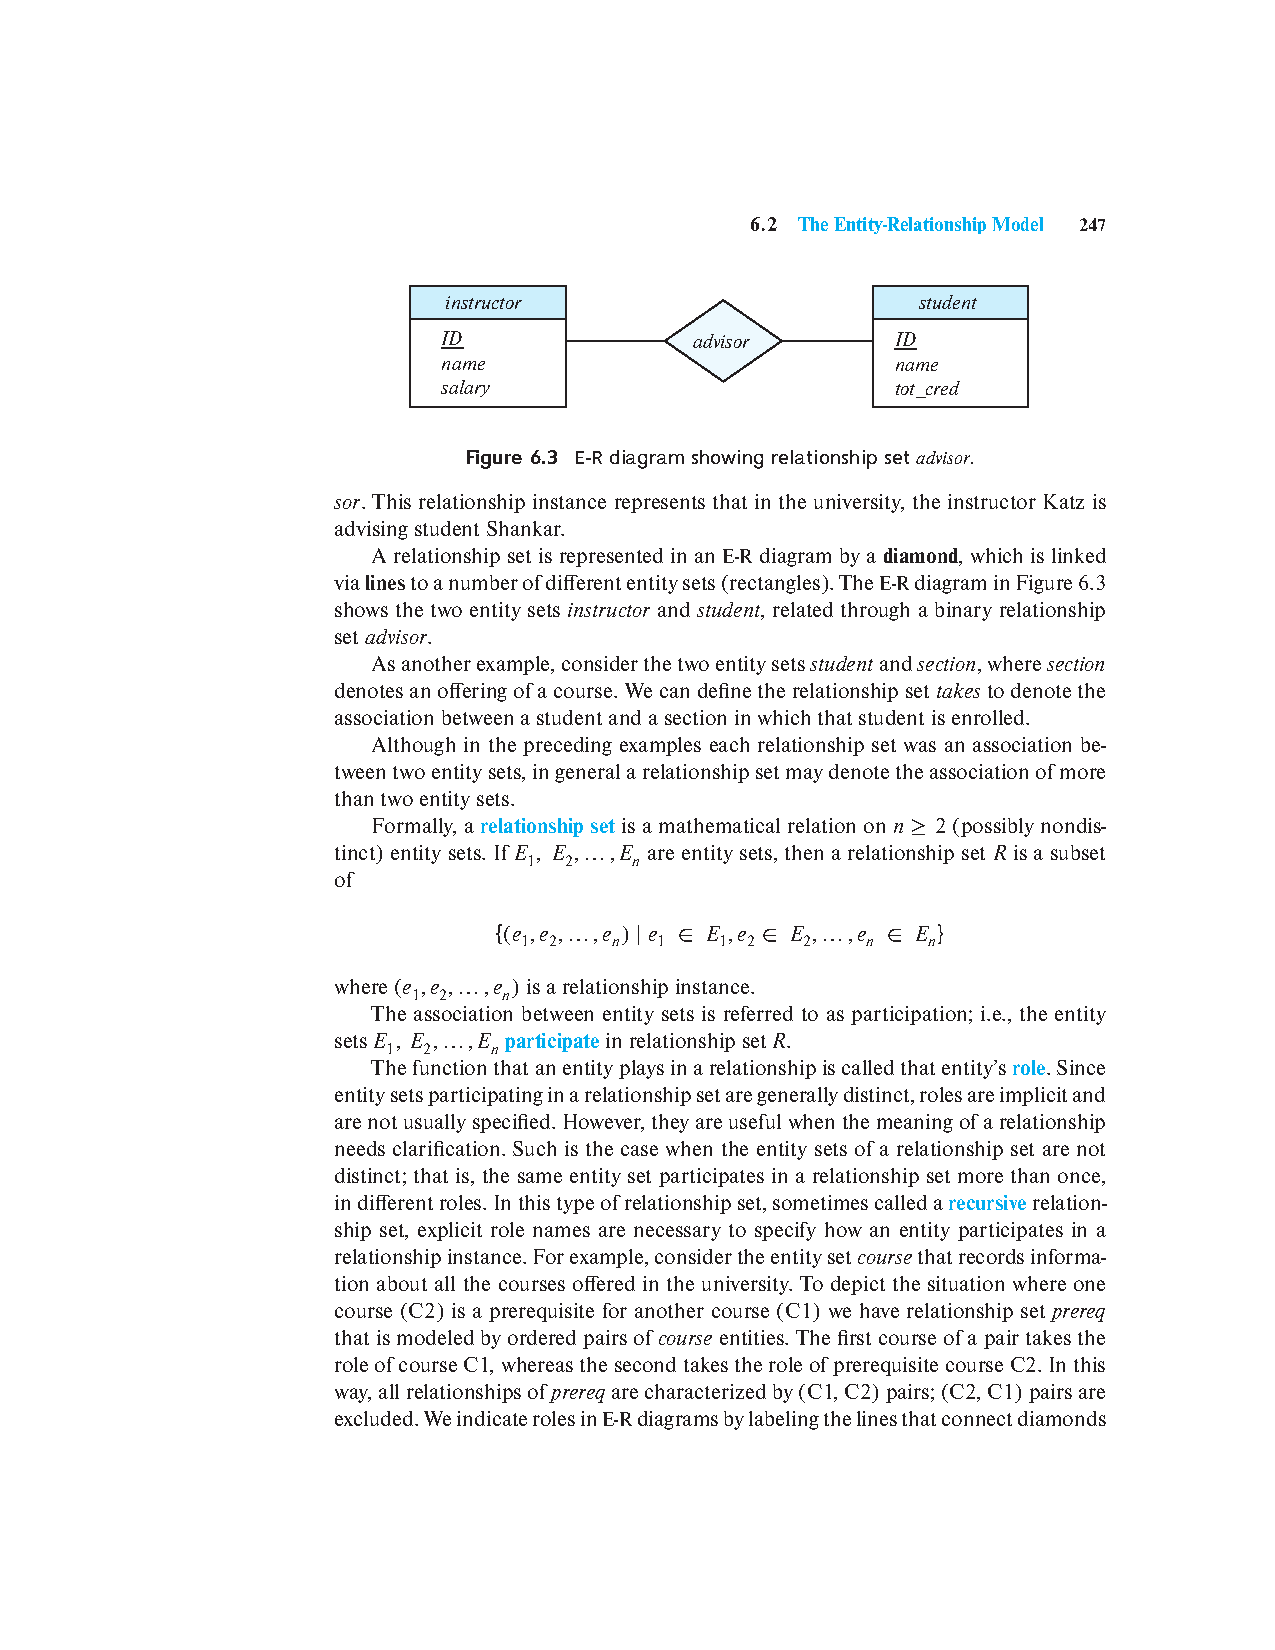
\includegraphics[trim={6.90cm 21cm 4.15cm 4cm}, clip, width=\textwidth]{figures/p247}
\end{frame}

\begin{frame}{Relationship Sets (Cont.)}
    \begin{itemize}
        \item An attribute can also be associated with a relationship set.
        \item For instance, the advisor relationship set between entity sets instructor and student may have the attribute date which tracks when the student started being associated with the advisor
    \end{itemize}
    \bigskip
    \centering
    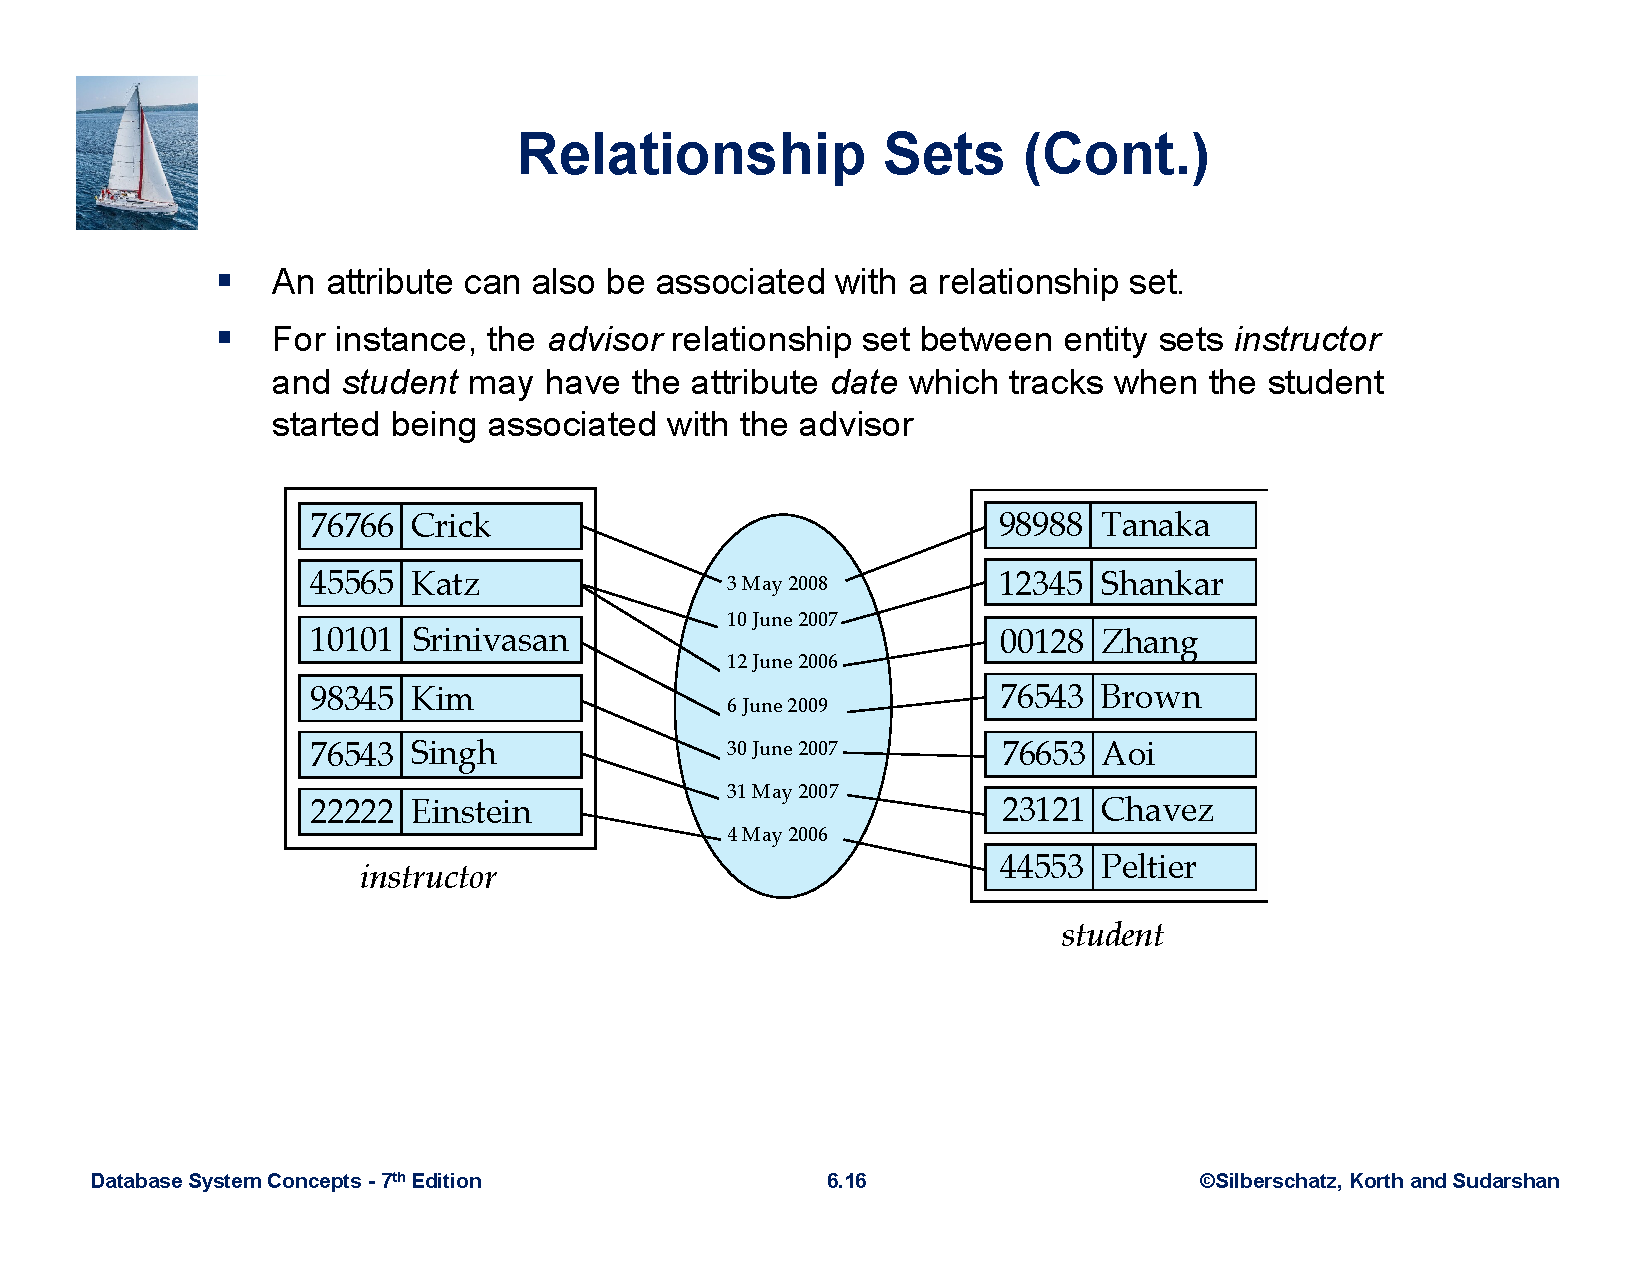
\includegraphics[trim={4.80cm 2cm 6.5cm 8cm}, clip, width=\textwidth]{figures/attr_rel}
\end{frame}

\begin{frame}{Relationship Sets with Attributes}
    \vspace{20mm}
    \centering
    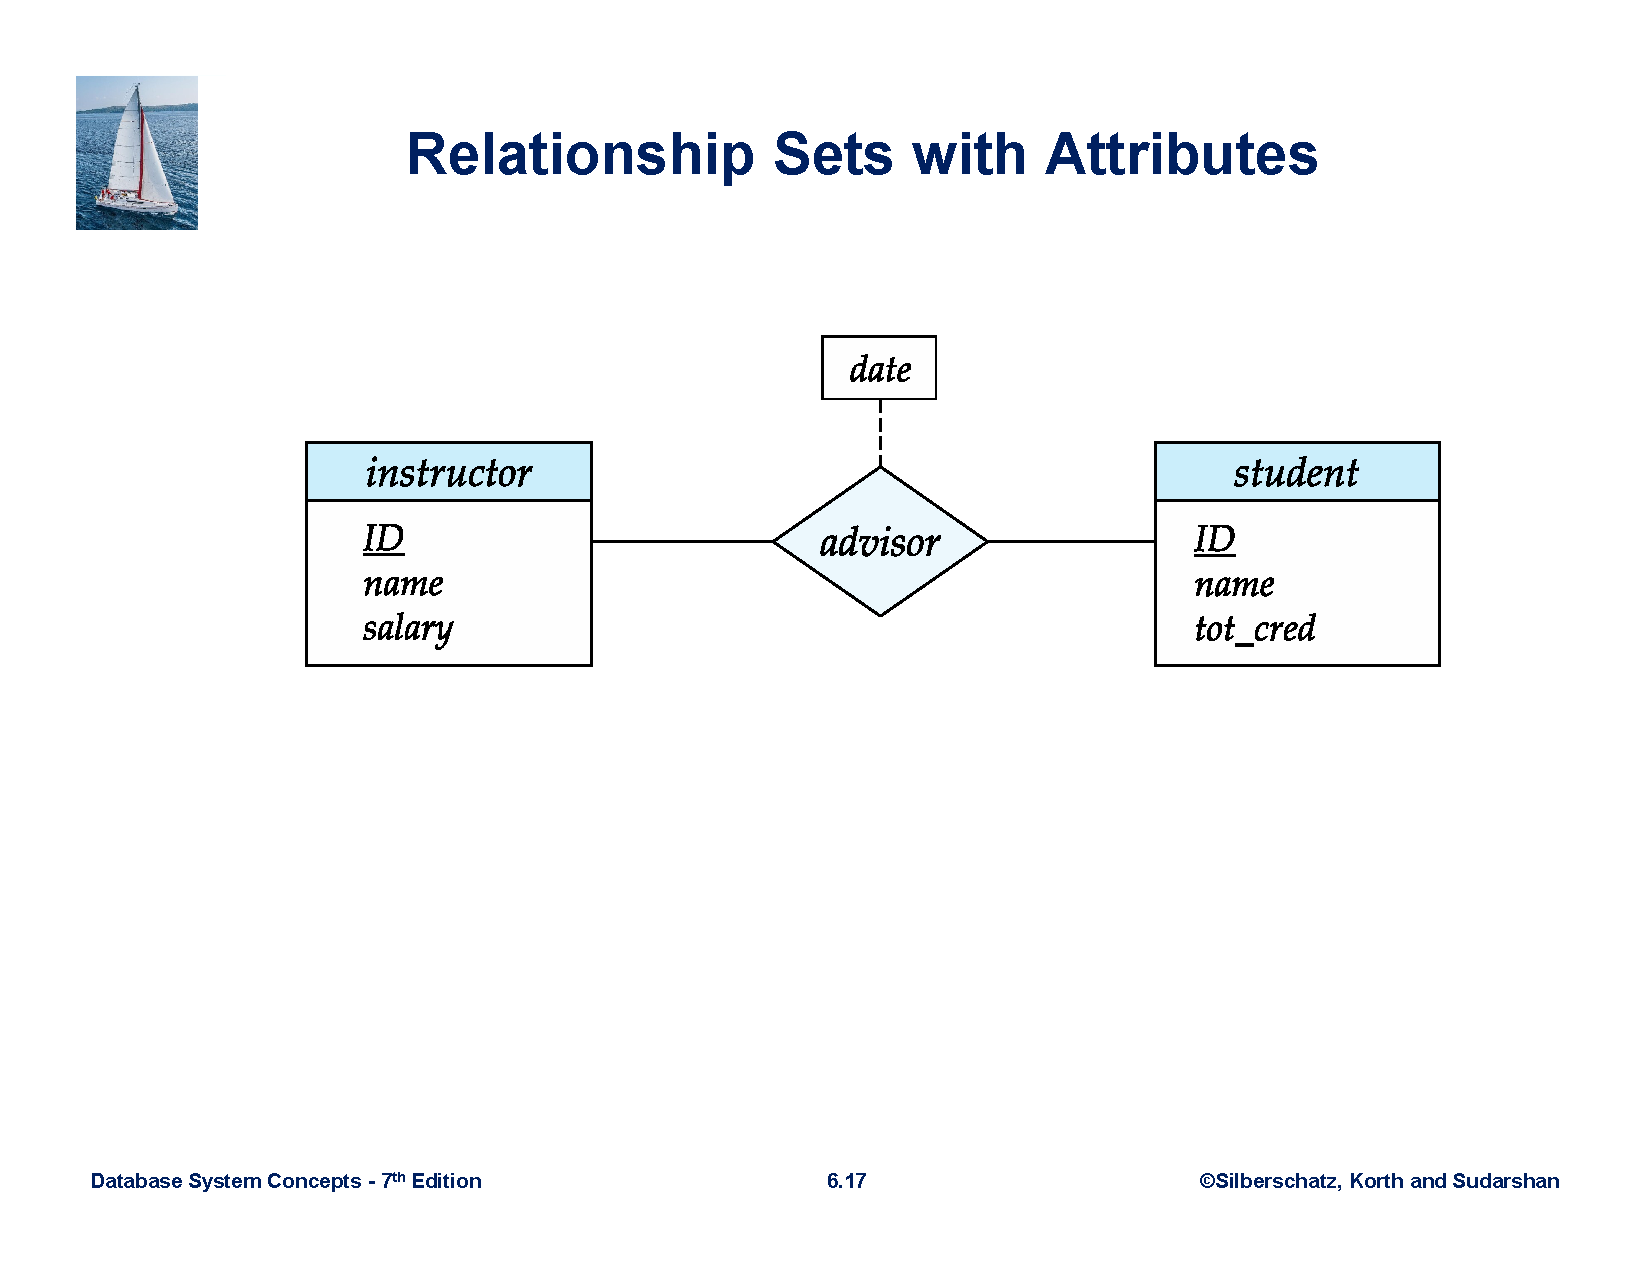
\includegraphics[trim={5.10cm 4cm 3.50cm 5.5cm}, clip, width=\textwidth]{figures/attr_rel2}
\end{frame}

\begin{frame}{Roles}
    \begin{itemize}
        \item Entity sets of a relationship need not be distinct.
        \begin{itemize}
            \item Each occurrence of an entity set plays a ``role'' in the relationship.
        \end{itemize}
        \item The labels \textit{``course\_id''} and \textit{``prereq\_id''} are called \textbf{roles}.
    \end{itemize}
    \centering
    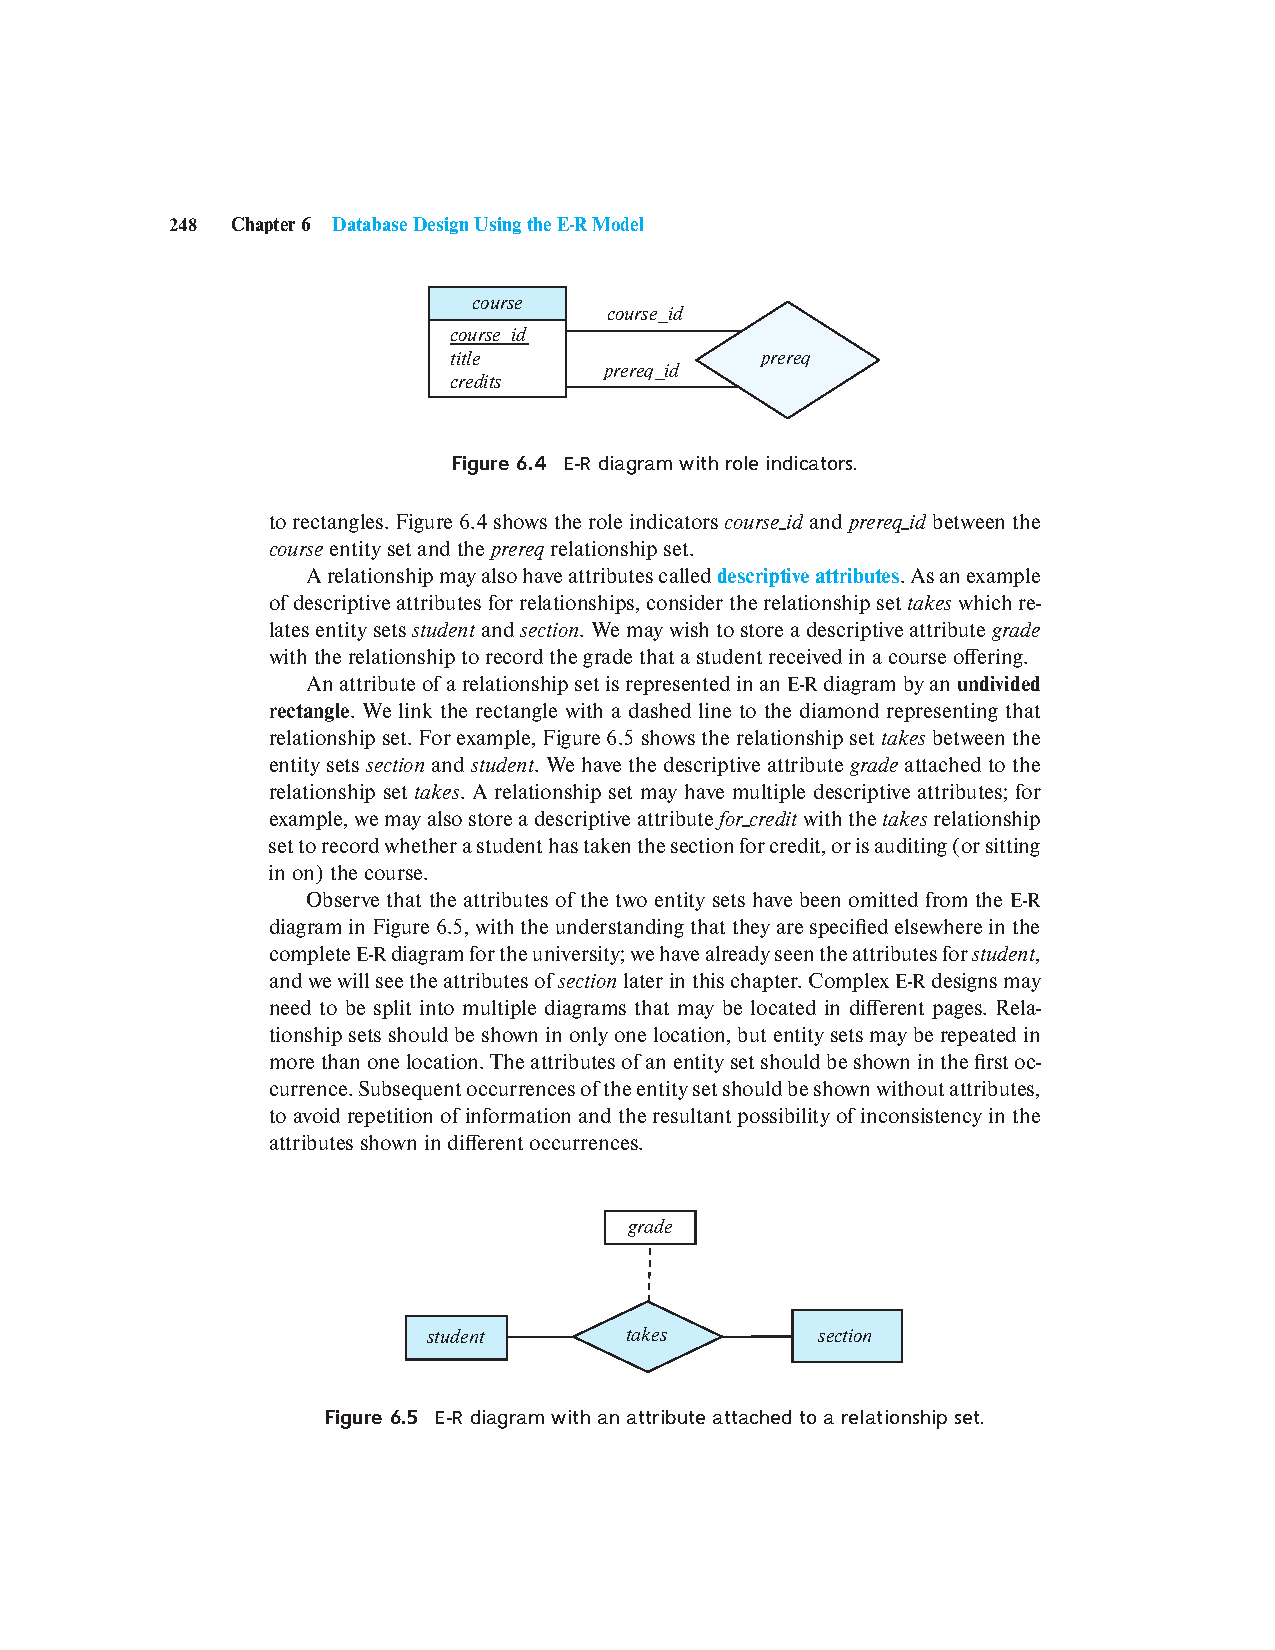
\includegraphics[trim={6.5cm 20.5cm 6.5cm 4cm}, clip, width=0.8\textwidth]{figures/p248}
\end{frame}

\begin{frame}{Degree of a Relationship Set}
    \begin{itemize}
        \item Binary relationship.
        \begin{itemize}
            \item involve two entity sets (or degree two).
            \item most relationship sets in a database system are binary.
        \end{itemize}
        \item Relationships between more than two entity sets are rare. Most relationships are binary. (More on this later.)
        \begin{itemize}
            \item Example: students work on research projects under the guidance of an instructor.
            \item relationship \textit{proj\_guide} is a ternary relationship between instructor, student, and project.
        \end{itemize}
    \end{itemize}
\end{frame}

\begin{frame}{Non-binary Relationship Sets}
    \begin{itemize}
        \item Most relationship sets are binary.
        \item There are occasions when it is more convenient to represent relationships as non-binary.
        \item E-R Diagram with a Ternary Relationship:
    \end{itemize}
    \centering
    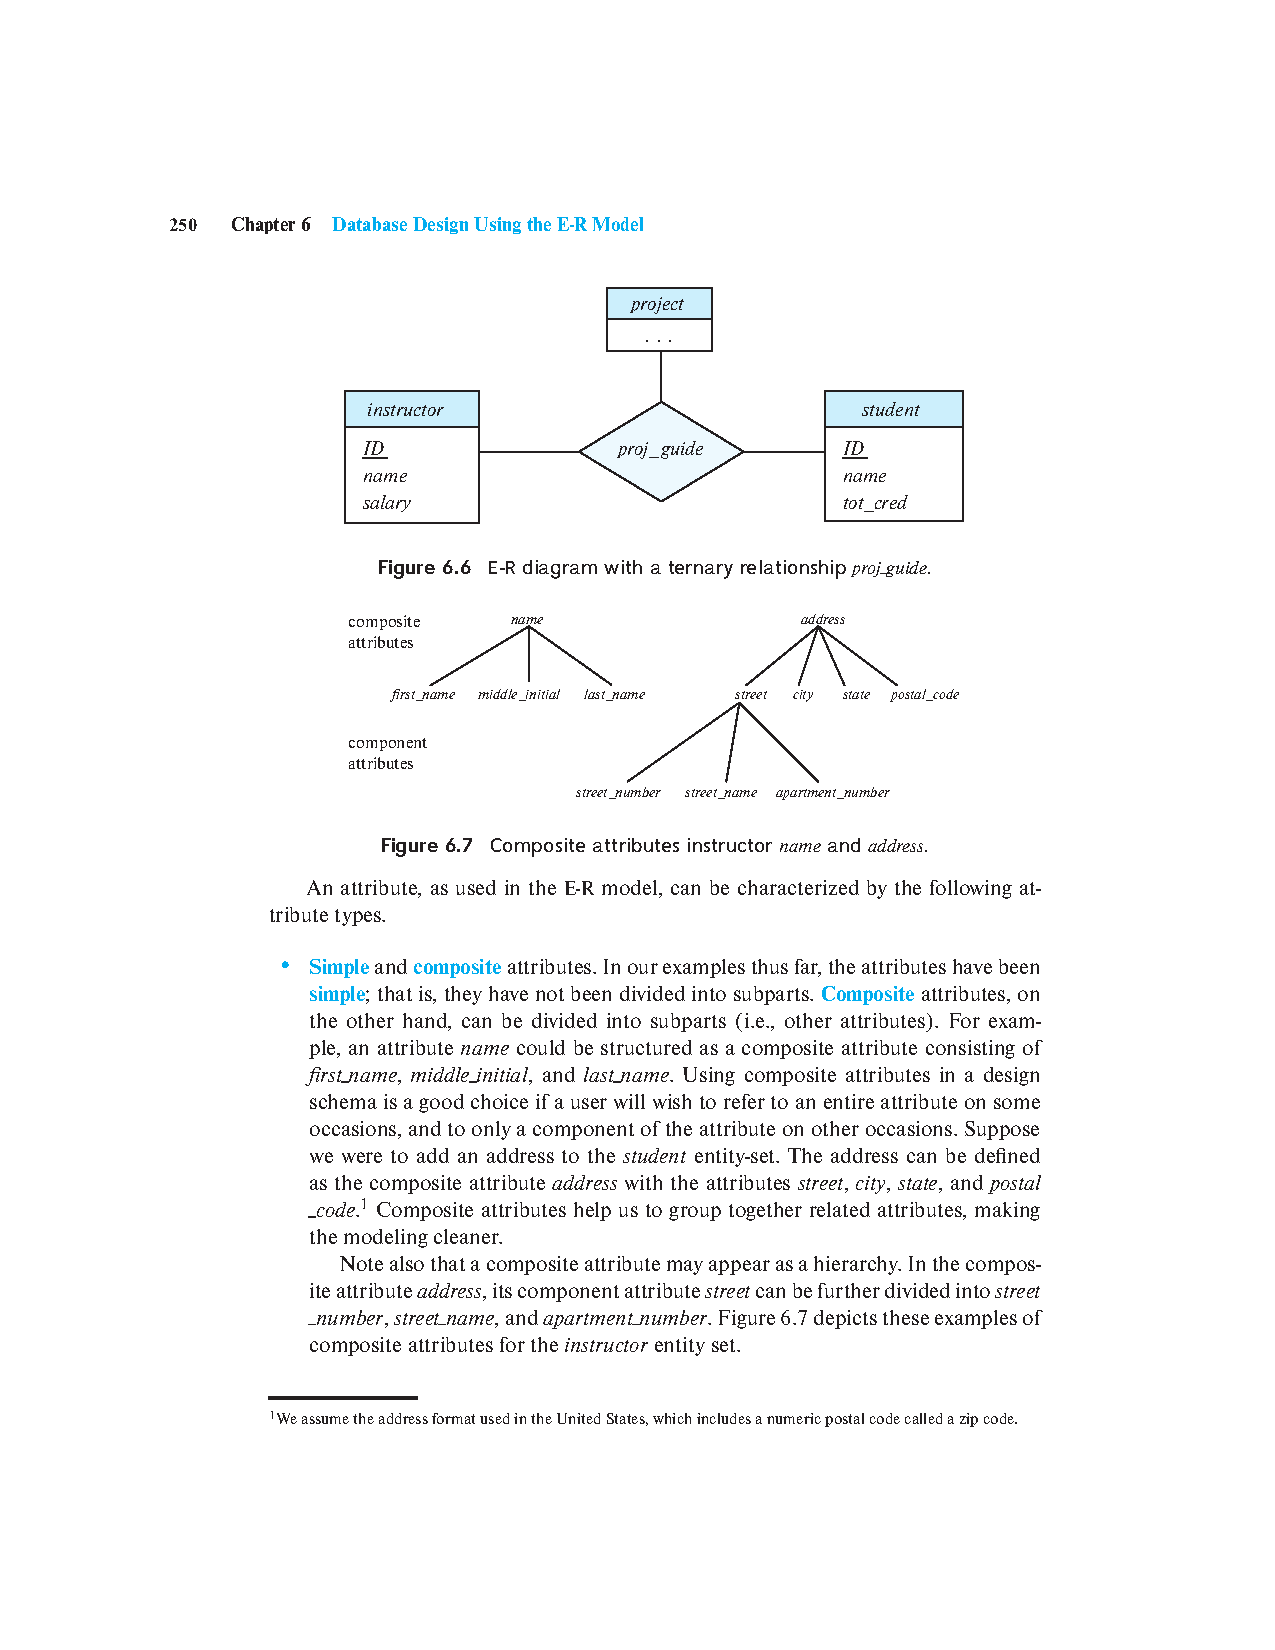
\includegraphics[trim={5cm 19cm 5cm 4cm}, clip, width=0.8\textwidth]{figures/p250}
\end{frame}

\section{Complex Attributes}

\begin{frame}{Complex Attributes}
    \begin{itemize}
        \item Attribute types:
        \begin{itemize}
            \item \textbf{Simple} and \textbf{composite} attributes.
            \item \textbf{Single-valued} and \textbf{multivalued} attributes.
            \begin{itemize}
                \item Example: multivalued attribute: phone\_numbers.
            \end{itemize}
            \item \textbf{Derived} attributes.
            \begin{itemize}
                \item Can be computed from other attributes.
                \item Example: age, given date\_of\_birth.
            \end{itemize}
        \end{itemize}
        \item \textbf{Domain} --the set of permitted values for each attribute.
    \end{itemize}
\end{frame}

\begin{frame}{Composite Attributes}
    \begin{itemize}
        \item Composite attributes allow us to divided attributes into subparts (other attributes).
    \end{itemize}
    \centering
    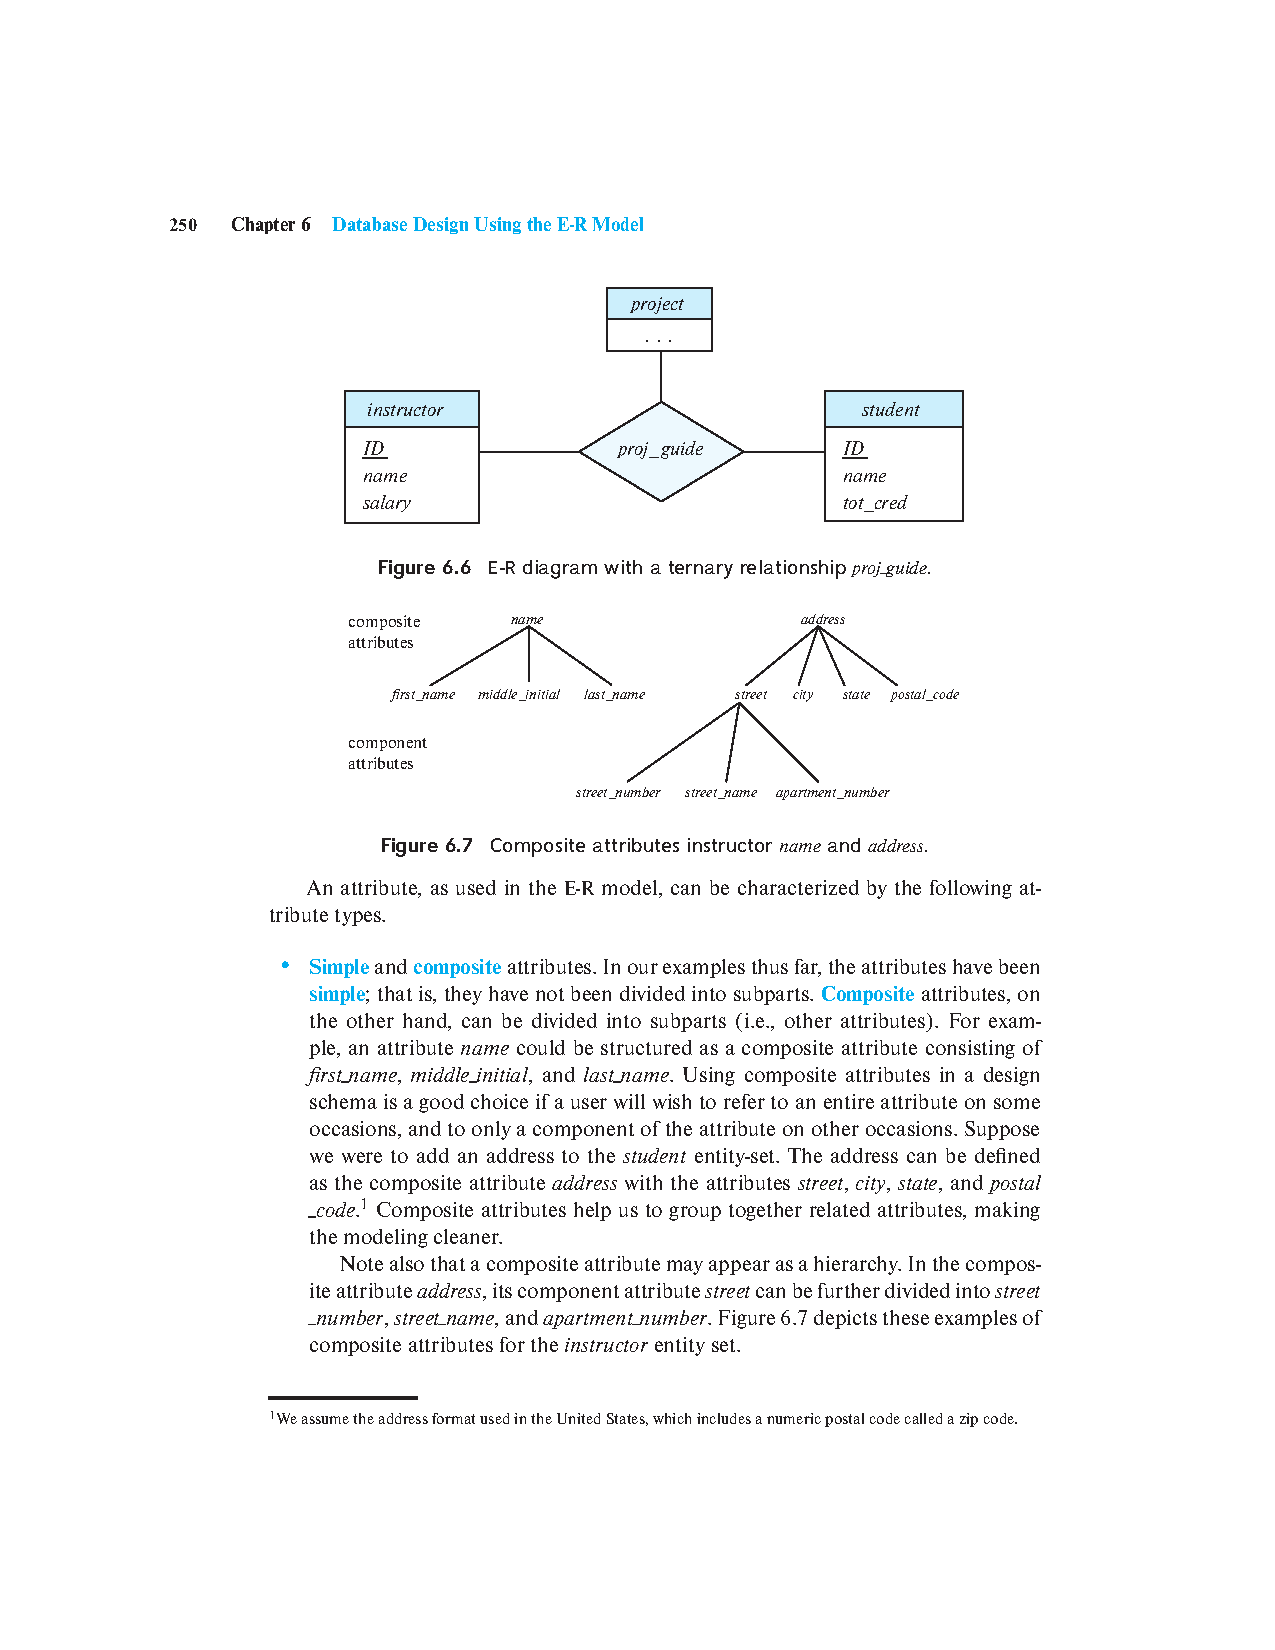
\includegraphics[trim={5cm 14cm 5cm 10cm}, clip, width=\textwidth]{figures/p250}
\end{frame}

\begin{frame}{Representing Complex Attributes in ER Diagram}
    \centering
    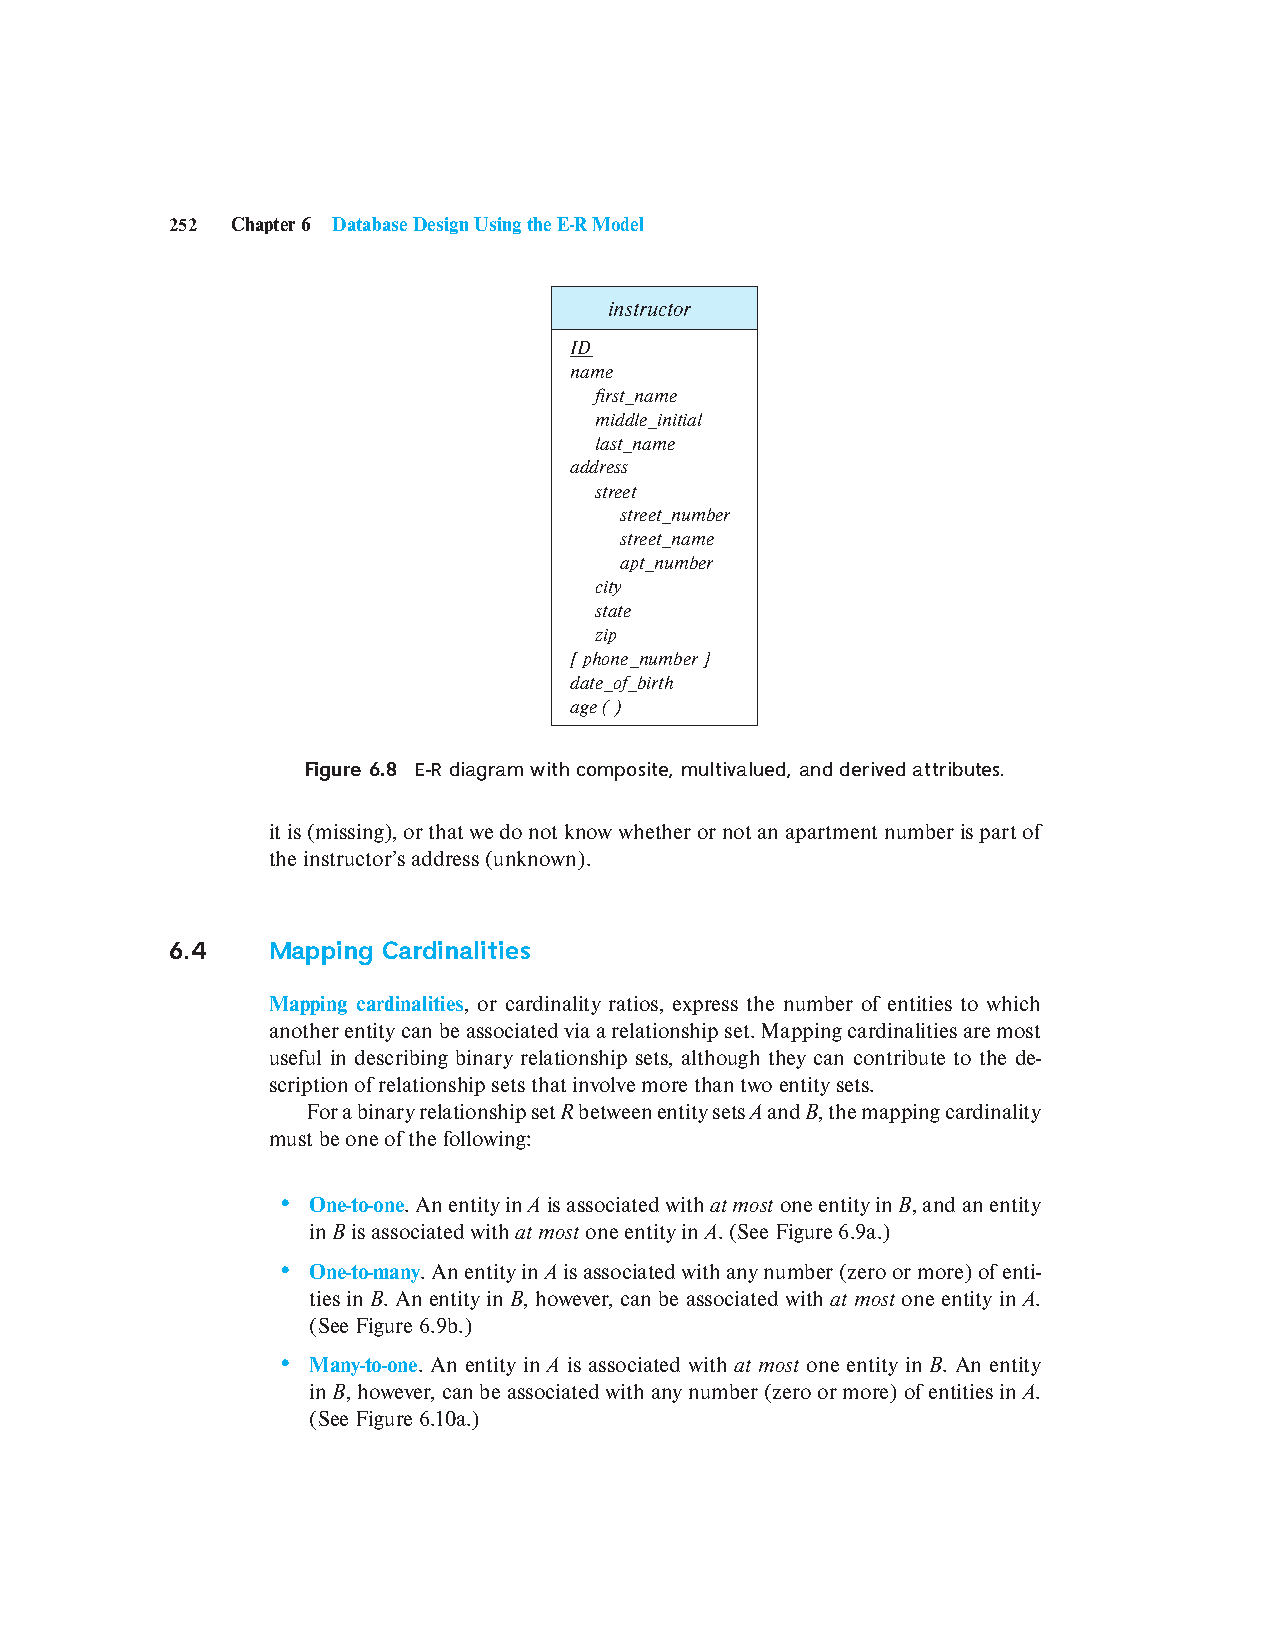
\includegraphics[trim={5cm 15.25cm 5cm 4cm}, clip, width=\textwidth]{figures/p252}
\end{frame}

\begin{frame}{Mapping Cardinality Constraints}
    \begin{itemize}
        \item Express the number of entities to which another entity can be associated via a relationship set.
        \item Most useful in describing binary relationship sets.
        \item For a binary relationship set the mapping cardinality must be one of the following types:
        \begin{itemize}
            \item One to one
            \item One to many
            \item Many to one
            \item Many to many
        \end{itemize}
    \end{itemize}
\end{frame}

\section{Mapping Cardinalities}

\begin{frame}{Mapping Cardinalities}
    \centering
    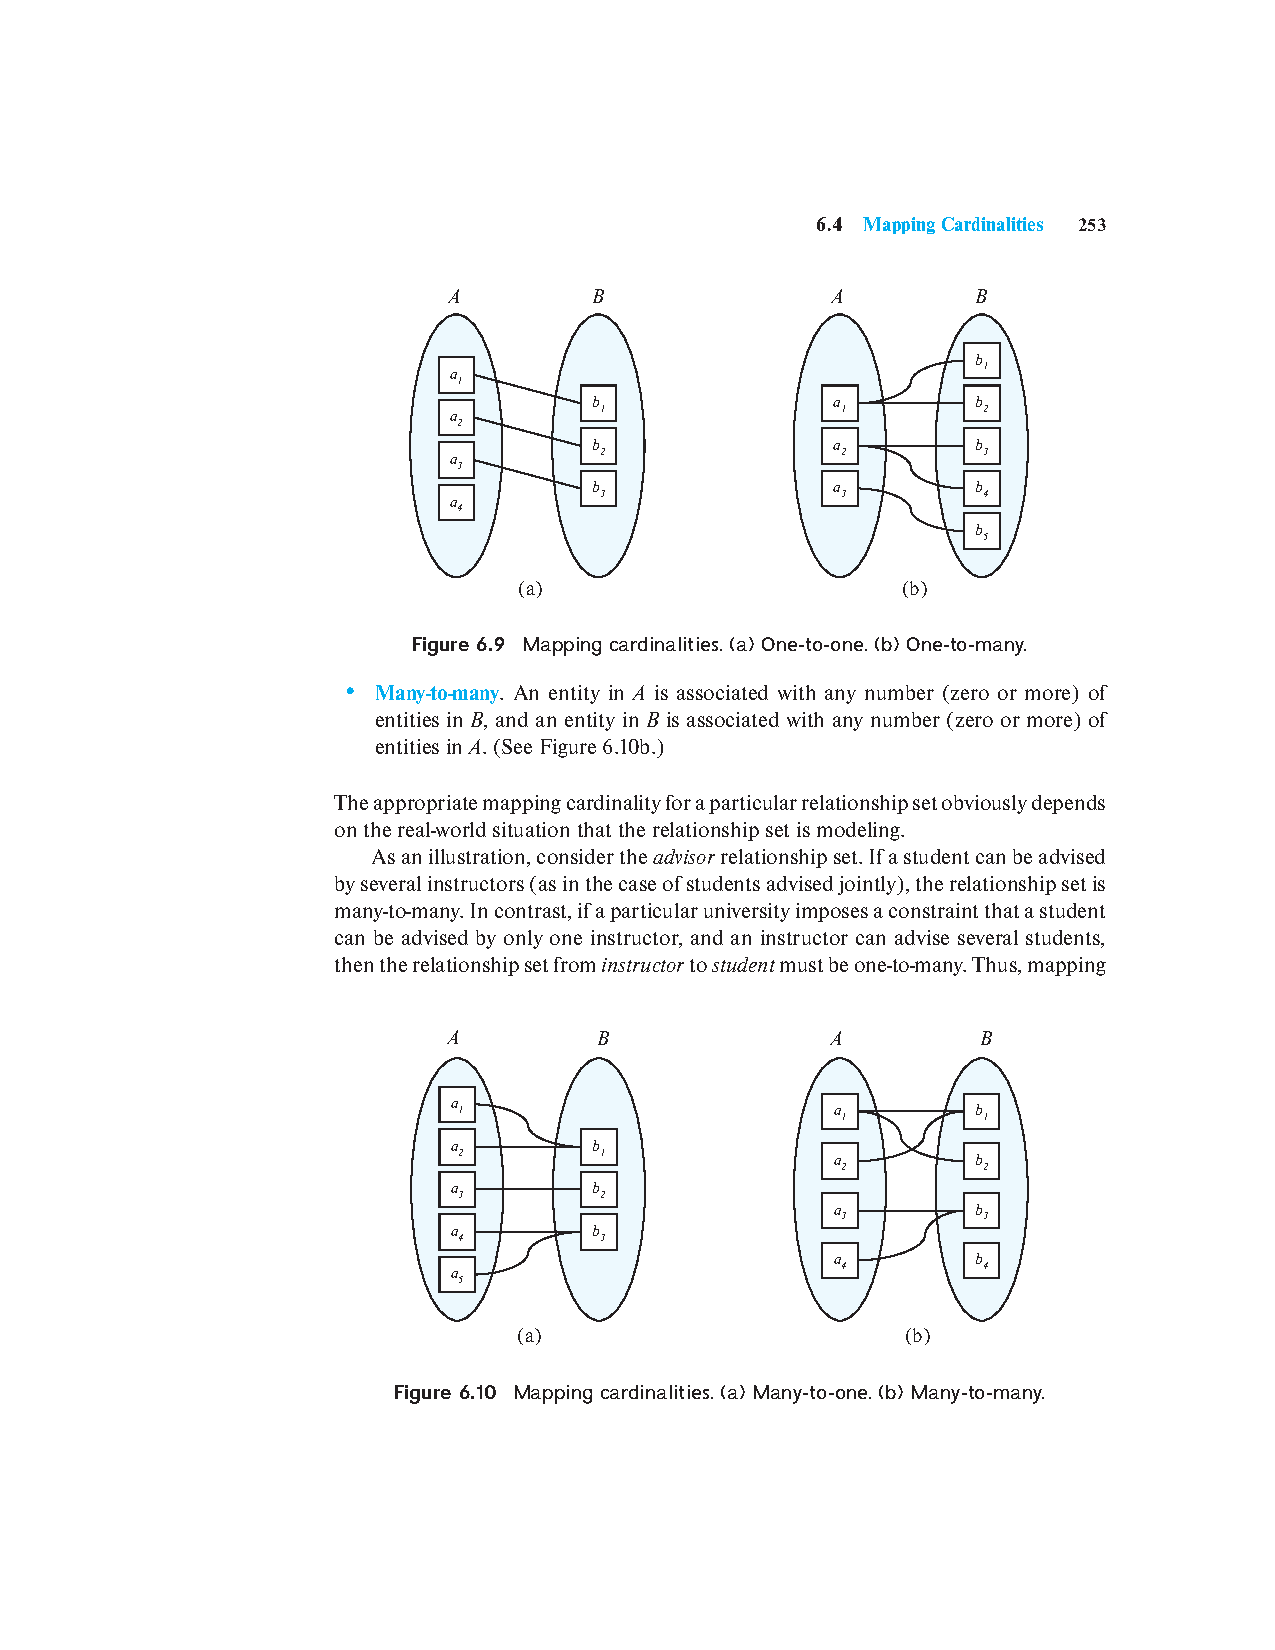
\includegraphics[trim={6.75cm 17.5cm 3.75cm 4cm}, clip, width=0.9\textwidth]{figures/p253}
    \begin{tabularx}{\textwidth}{@{} Y Y @{}}
        one to one & one to many \\
    \end{tabularx}
    \begin{block}{Note:}
        Some elements in A and B may not be mapped to any elements in the other set.
    \end{block}
\end{frame}

\begin{frame}{Mapping Cardinalities}
    \centering
    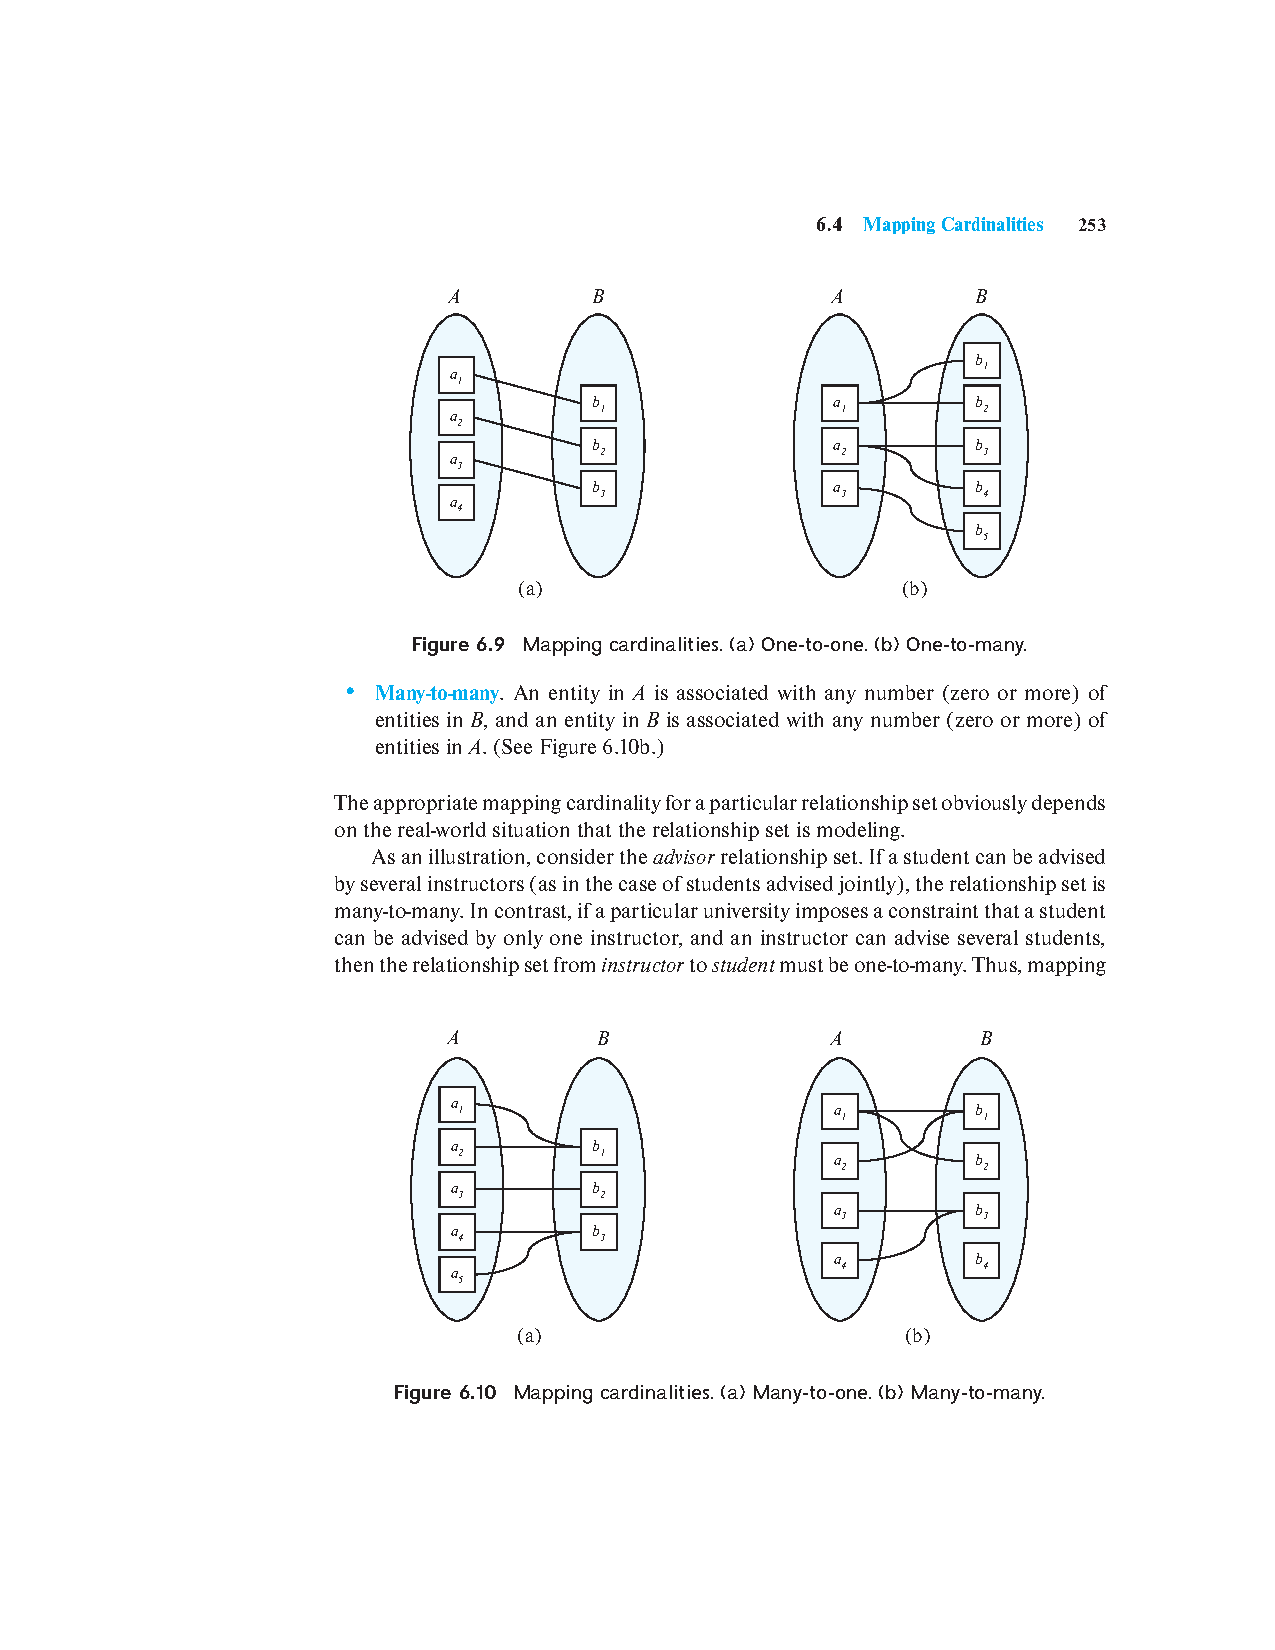
\includegraphics[trim={6.75cm 5cm 3.75cm 17cm}, clip, width=0.9\textwidth]{figures/p253}
    \begin{tabularx}{\textwidth}{@{} Y Y @{}}
        many to one & many to many \\
    \end{tabularx}
    \begin{block}{Note:}
        Some elements in A and B may not be mapped to any elements in the other set.
    \end{block}
\end{frame}

\begin{frame}{Representing Cardinality Constraints in ER Diagram}
    \begin{itemize}
        \item We express cardinality constraints by drawing either a directed line ($\rightarrow$), signifying ``one,'' or an undirected line (\textemdash), signifying ``many,'' between the relationship set and the entity set.
        \item One-to-one relationship between an \textit{instructor} and a \textit{student}:
        \begin{itemize}
            \item A student is associated with at most one instructor via the relationship advisor.
            \item An instructor is associated with at most one student via the relationship advisor.
        \end{itemize}
    \end{itemize}
    \centering
    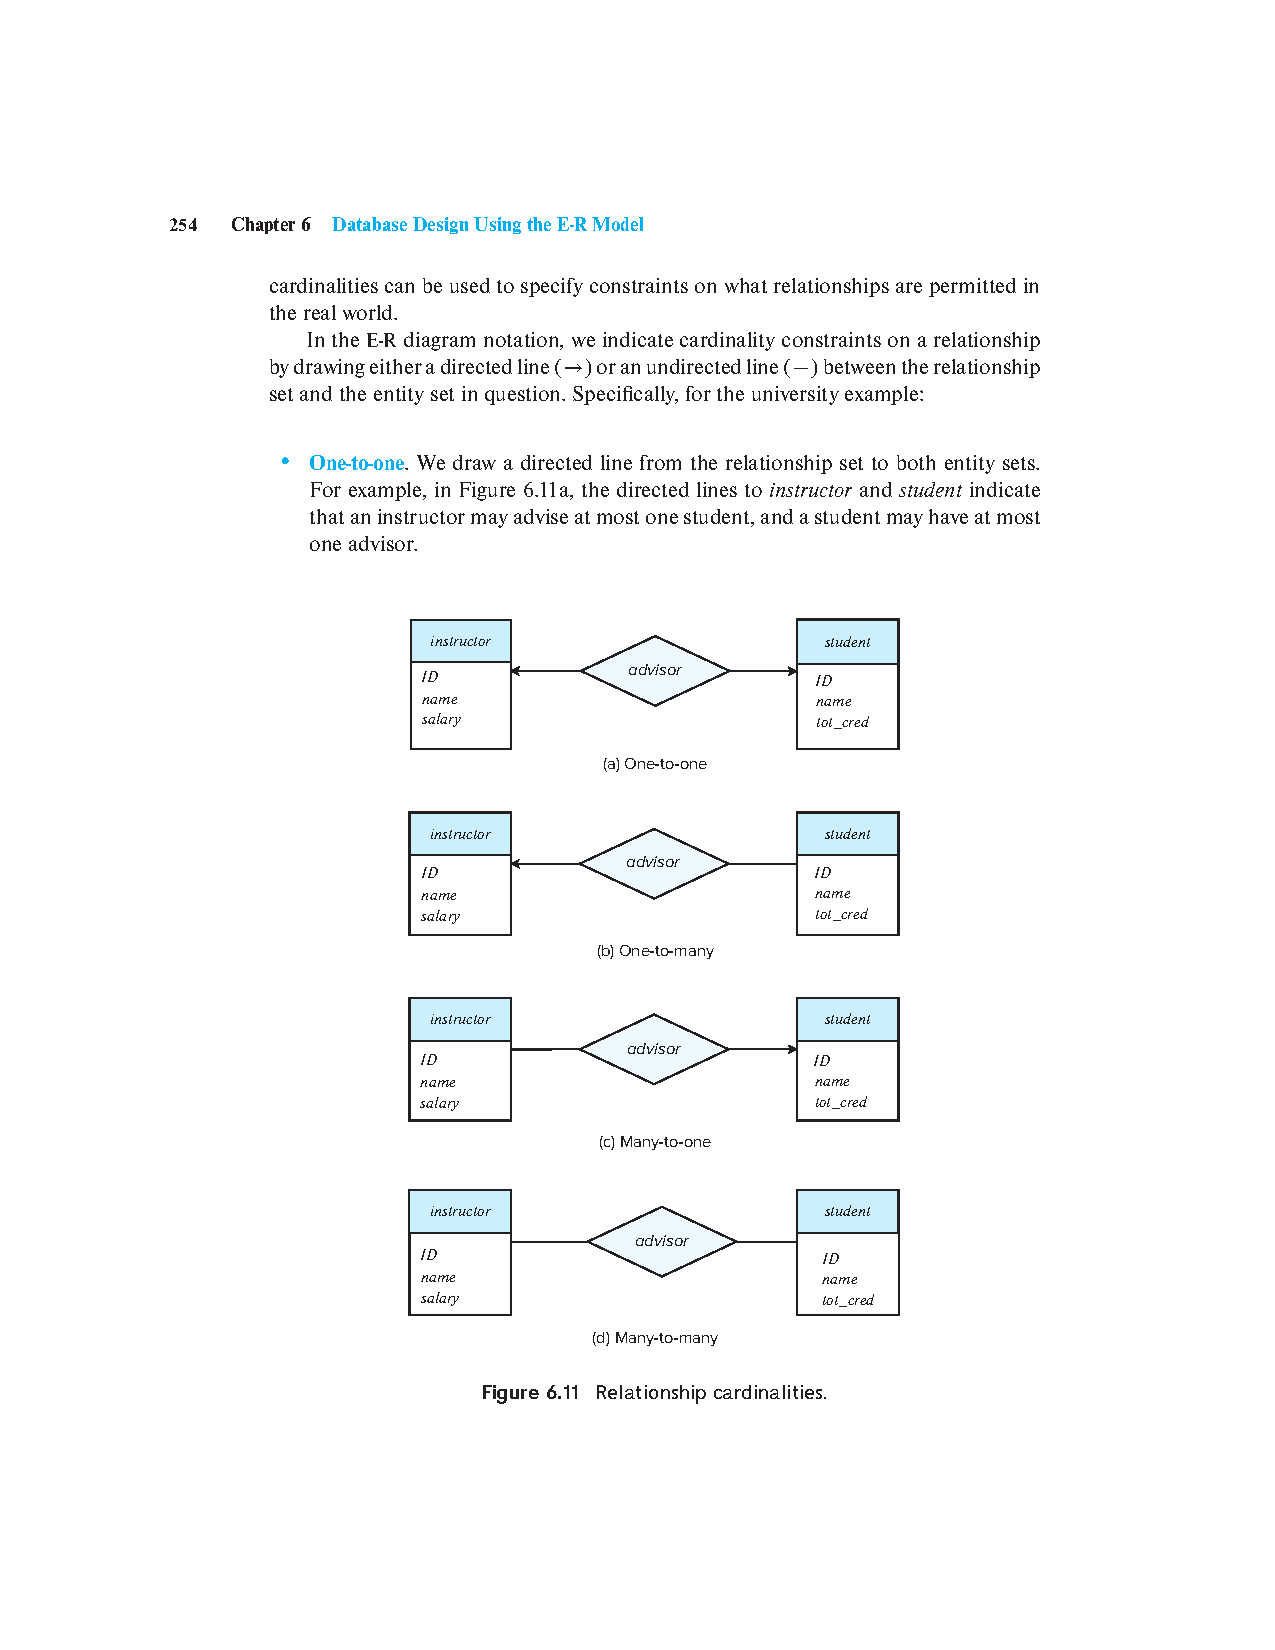
\includegraphics[trim={6cm 15.20cm 6cm 10cm}, clip, width=0.9\textwidth]{figures/p254}
\end{frame}

\begin{frame}{One-to-Many Relationship}
    \begin{itemize}
        \item In a one-to-many relationship between an instructor and a student:
        \begin{itemize}
            \item an instructor is associated with several (including 0) students via advisor.
            \item a student is associated with at most one instructor via advisor.
        \end{itemize}
    \end{itemize}
    \centering
    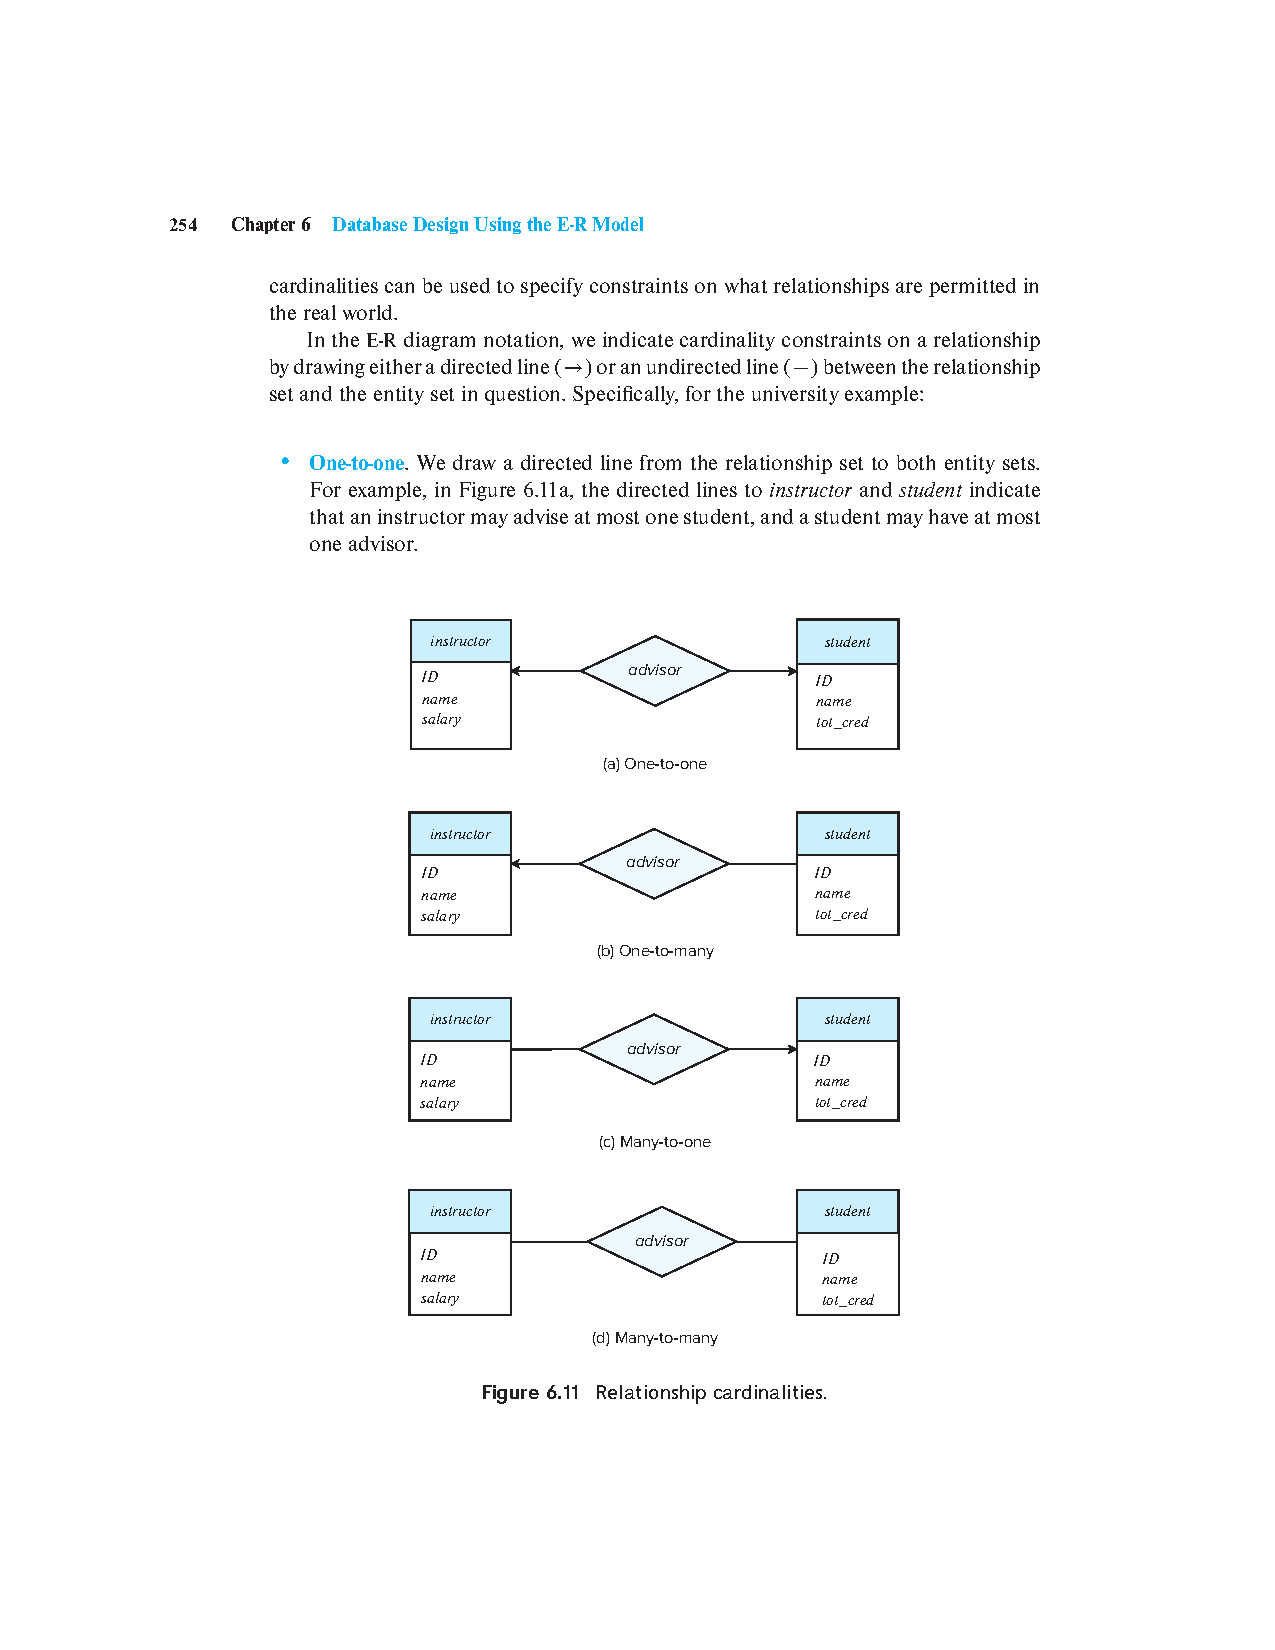
\includegraphics[trim={6cm 12cm 6cm 13.25cm}, clip, width=0.9\textwidth]{figures/p254}
\end{frame}

\begin{frame}{Many-to-One Relationship}
    \begin{itemize}
        \item In a many-to-one relationship between an instructor and a student:
        \begin{itemize}
            \item an instructor is associated with at most one student via advisor.
            \item a student is associated with several (including 0) instructors via advisor.
        \end{itemize}
    \end{itemize}
    \centering
    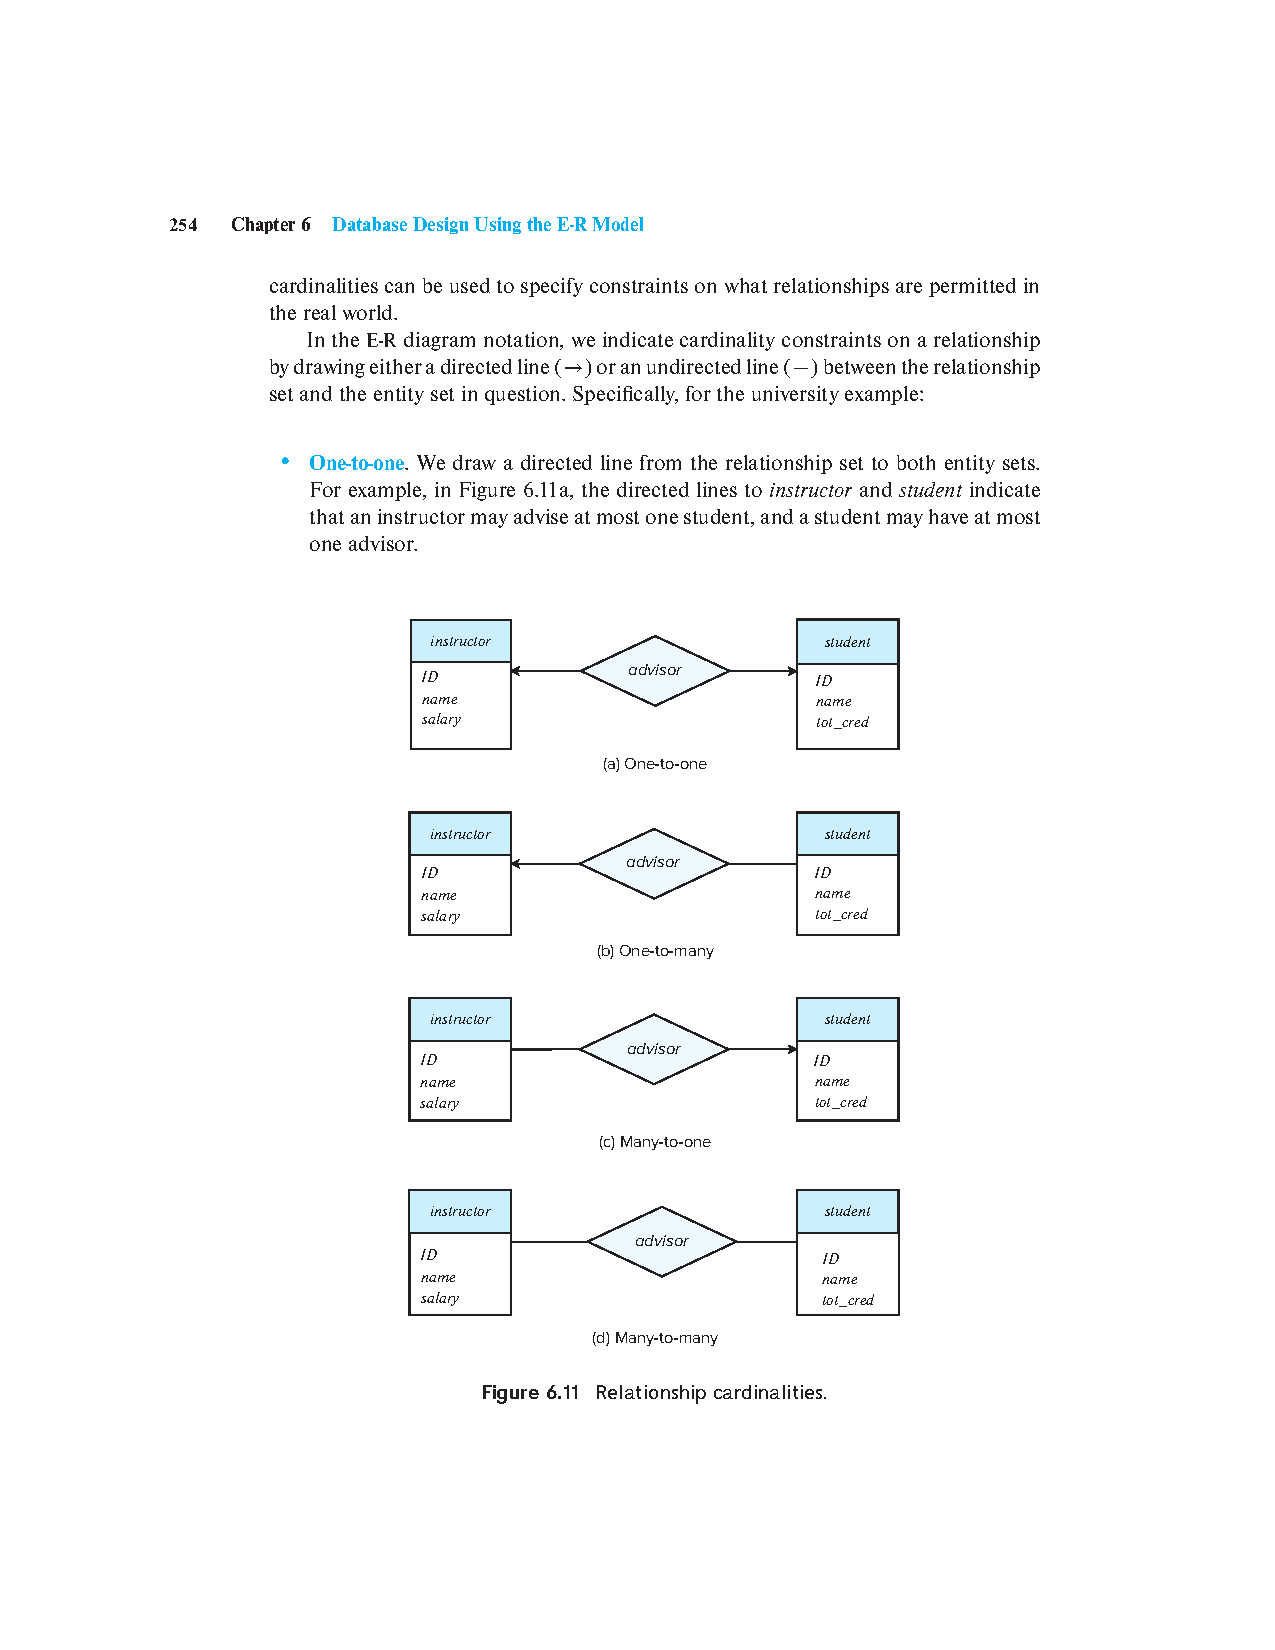
\includegraphics[trim={6cm 8.75cm 6cm 16.5cm}, clip, width=0.9\textwidth]{figures/p254}
\end{frame}

\begin{frame}{Many-to-Many Relationship}
    \begin{itemize}
        \item In a many-to-many relationship between an instructor and a student:
        \begin{itemize}
            \item an instructor is associated with several (possibly 0) students via advisor.
            \item a student is associated with several (possibly 0) instructors via advisor.
        \end{itemize}
    \end{itemize}
    \centering
    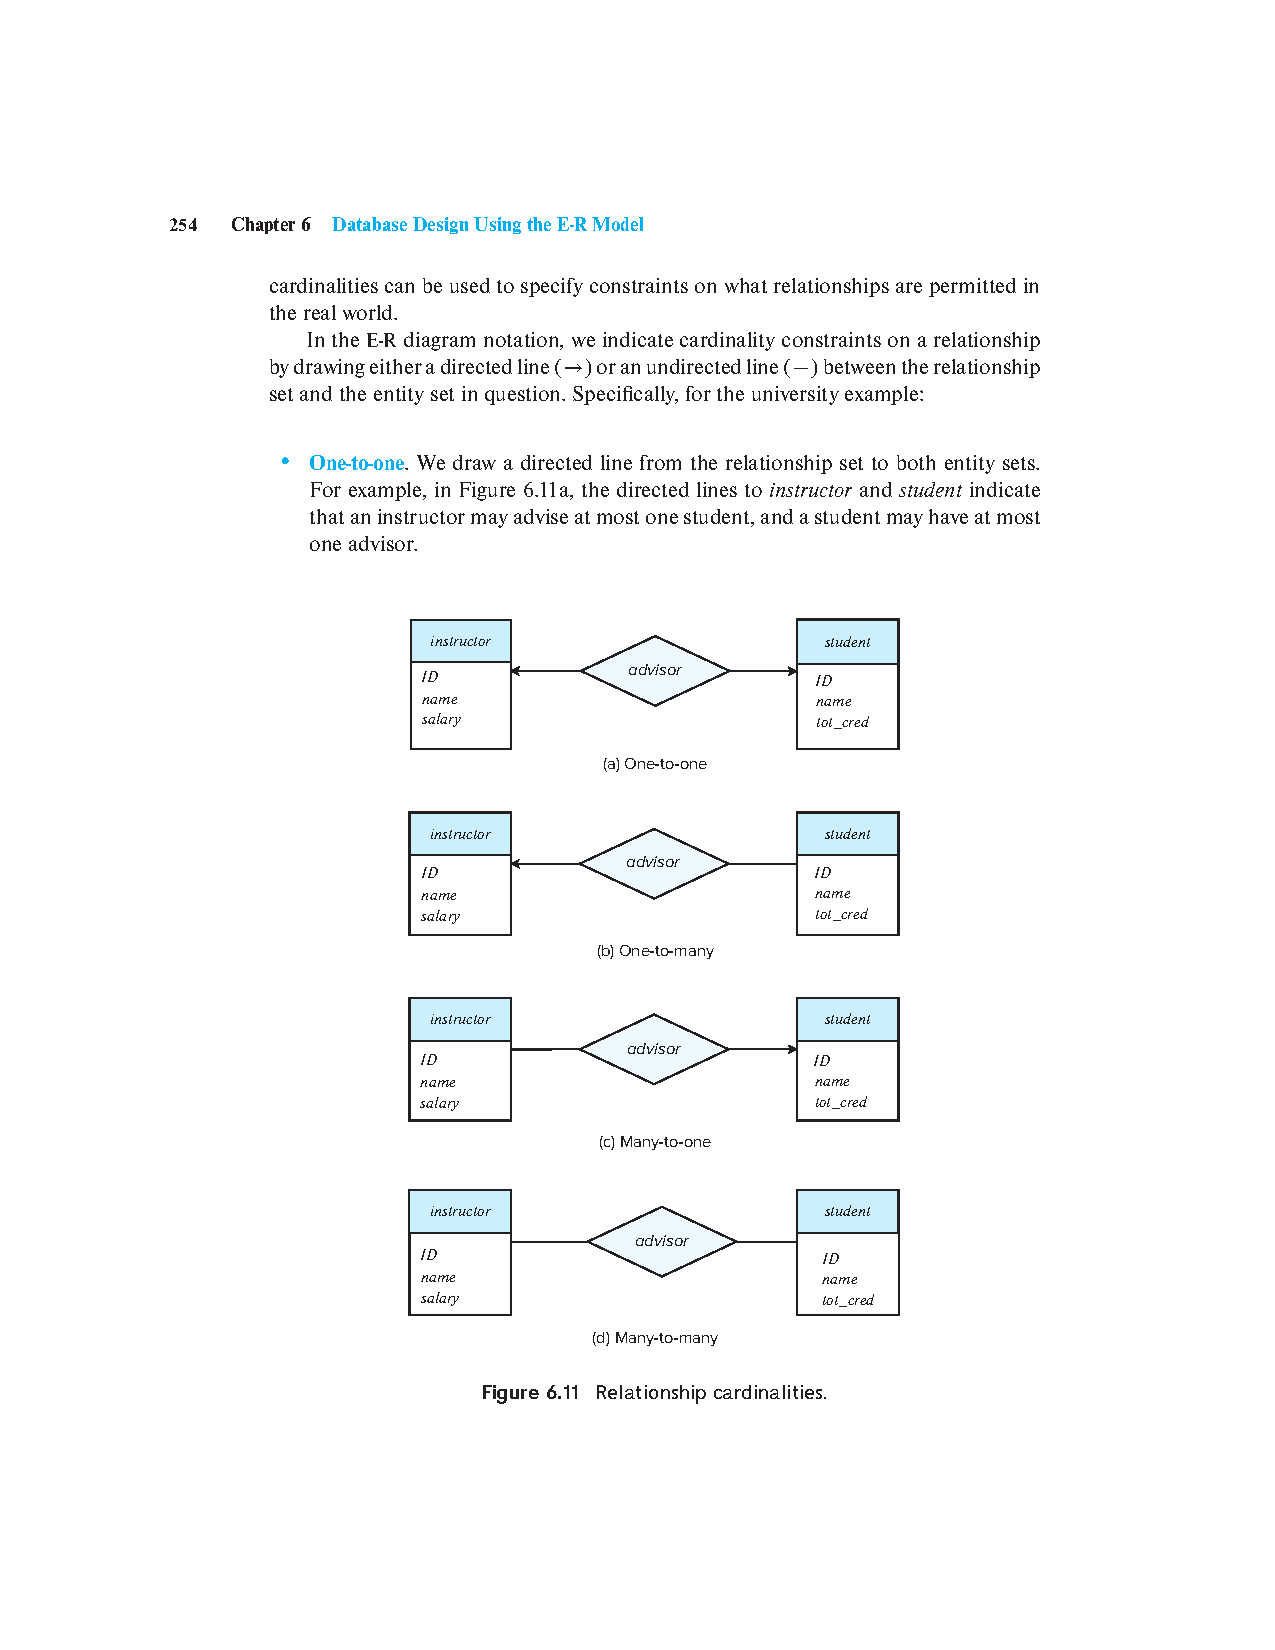
\includegraphics[trim={6cm 5.5cm 6cm 19.75cm}, clip, width=0.9\textwidth]{figures/p254}
\end{frame}

\begin{frame}{Total and Partial Participation}
    \begin{itemize}
        \item \textbf{Total participation} (indicated by double line): every entity in the entity set participates in at least one relationship in the relationship set. \\
        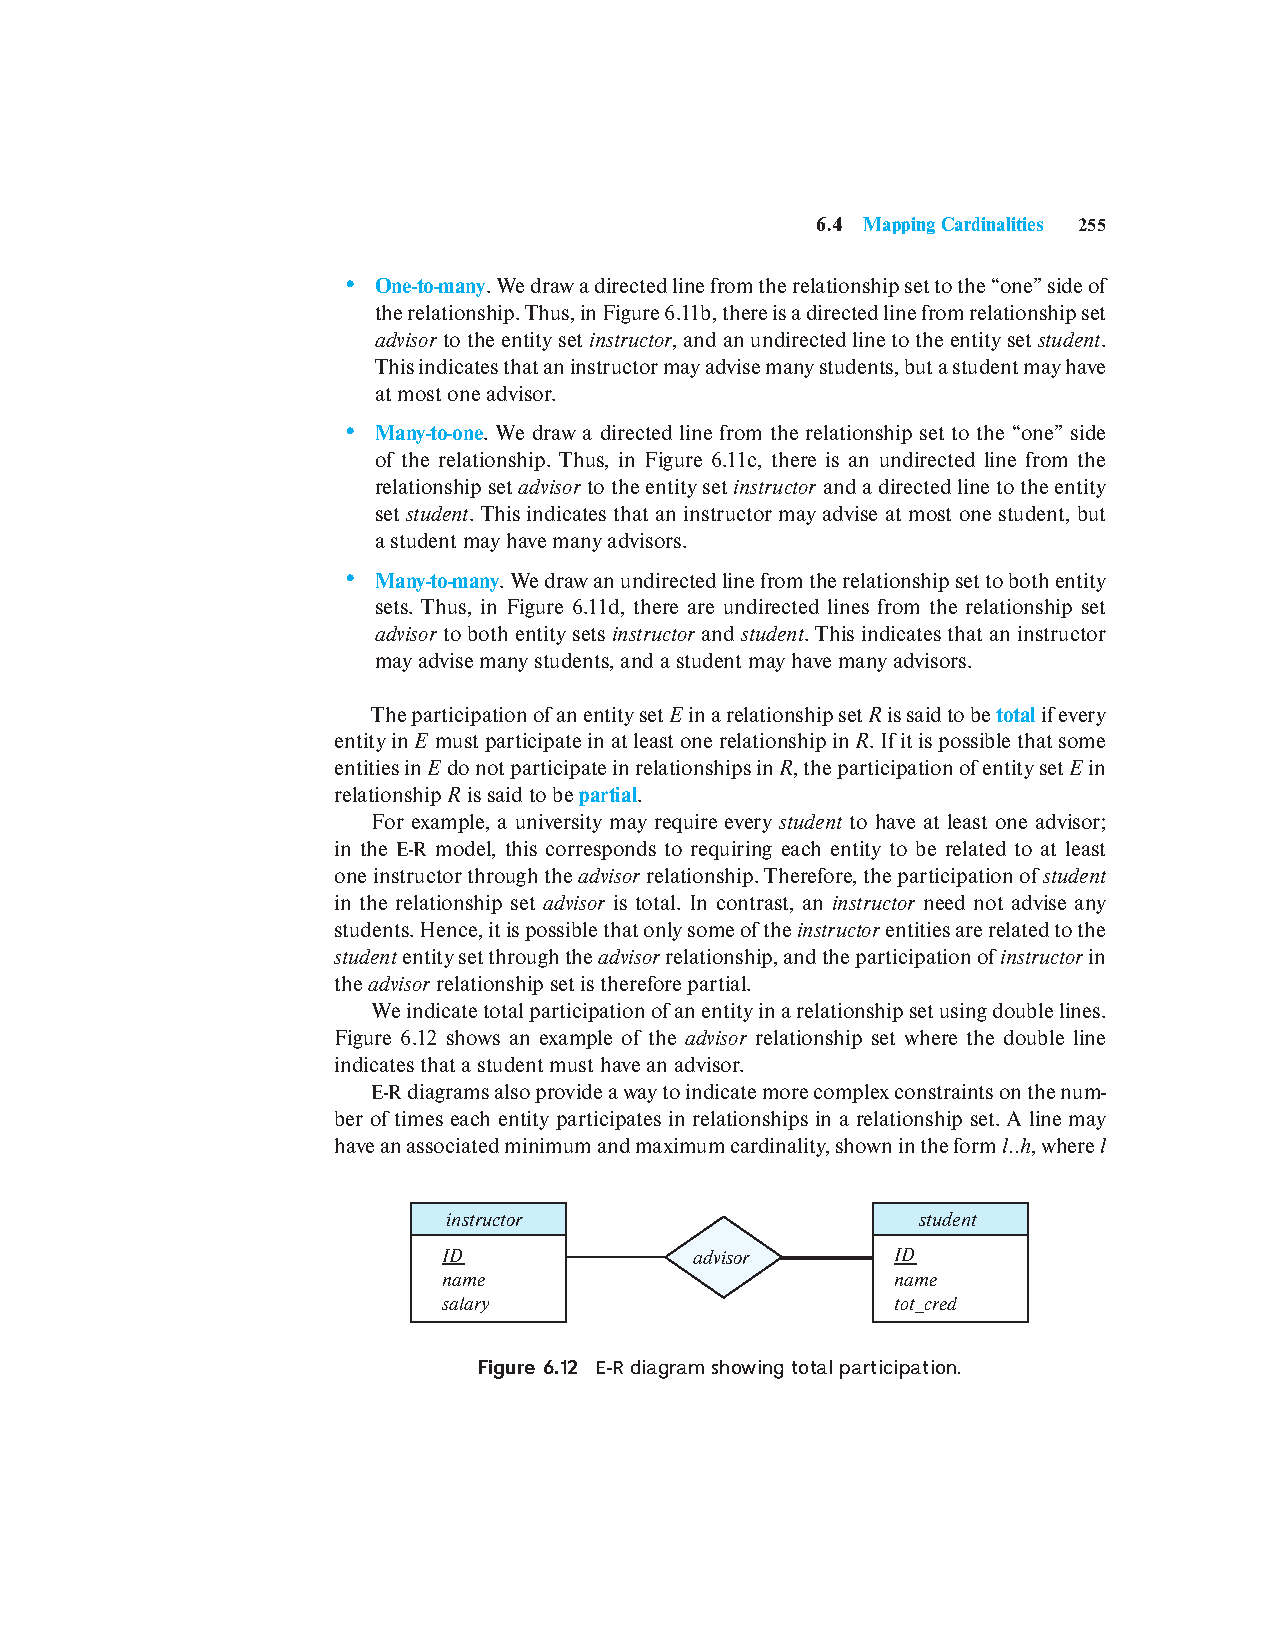
\includegraphics[trim={6cm 5.5cm 4cm 19.75cm}, clip, width=0.9\textwidth]{figures/p255}\\
        participation of student in advisor relation is total.
        \begin{itemize}
            \item every student must have an associated instructor.
        \end{itemize}
        \item \textbf{Partial participation}: some entities may not participate in any relationship in the relationship set.
        \begin{itemize}
            \item Example: participation of instructor in advisor is partial.
        \end{itemize}
    \end{itemize}
\end{frame}

\begin{frame}{Notation for Expressing More Complex Constraints}
    \begin{itemize}
        \item A line may have an associated minimum and maximum cardinality, shown in the form $l..h$, where $l$ is the minimum and $h$ the maximum cardinality.
        \begin{itemize}
            \item A minimum value of 1 indicates total participation.
            \item A maximum value of 1 indicates that the entity participates in at most one relationship.
            \item A maximum value of * indicates no limit.
        \end{itemize}
        \item Example: Instructor can advise 0 or more students. A student must have 1 advisor; cannot have multiple advisors.
            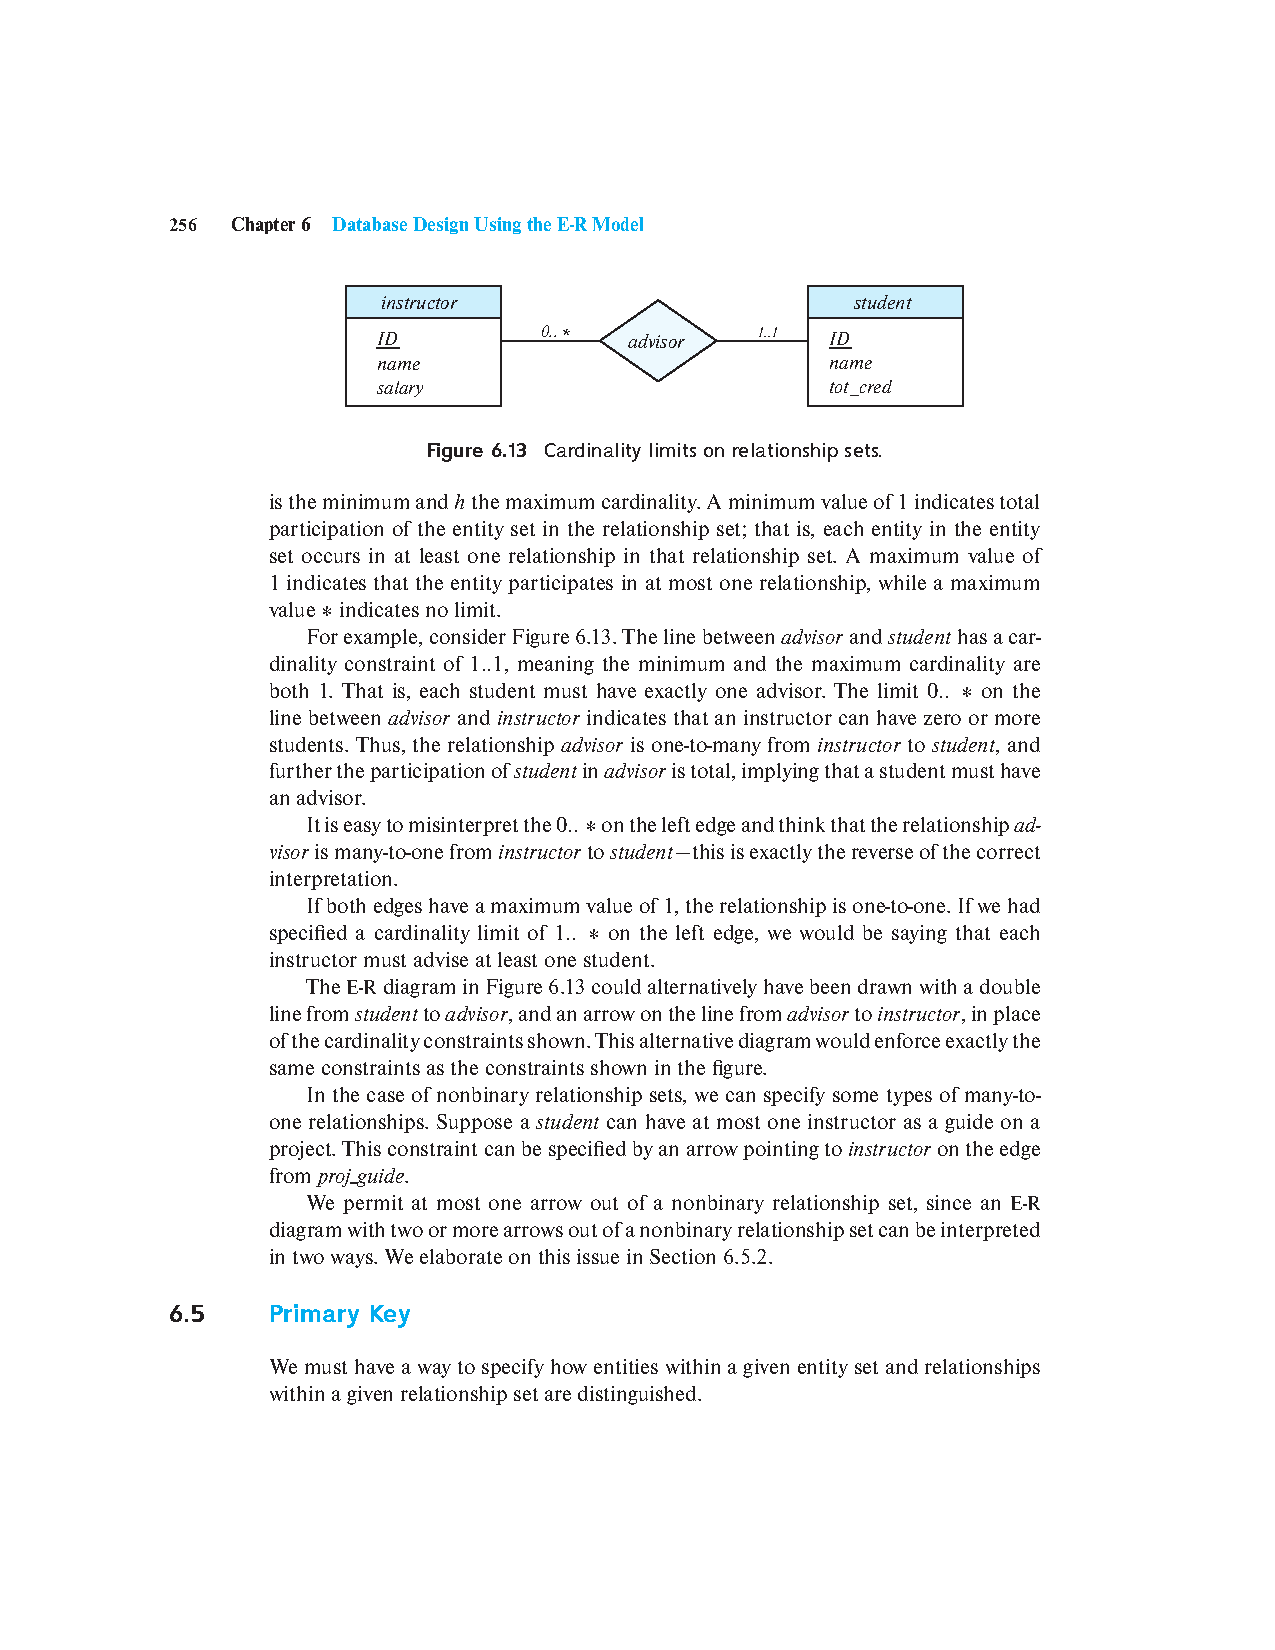
\includegraphics[trim={5cm 21cm 5cm 4.25cm}, clip, width=0.9\textwidth]{figures/p256}
    \end{itemize}
\end{frame}

\begin{frame}{Cardinality Constraints on Ternary Relationship}
    \begin{itemize}
        \item We allow at most one arrow out of a ternary (or greater degree) relationship to indicate a cardinality constraint.
        \item For example, an arrow from proj\_guide to instructor indicates each student has at most one guide for a project.
        \item If there is more than one arrow, there are two ways of defining the meaning.
        \begin{itemize}
            \item For example, a ternary relationship R between A, B and C with arrows to B and C could mean:
            \begin{enumerate}
                \item Each A entity is associated with a unique entity from B and C or
                \item Each pair of entities from (A, B) is associated with a unique C entity, and each pair (A, C) is associated with a unique B.
            \end{enumerate}
            \item Each alternative has been used in different formalisms.
            \item To avoid confusion we outlaw more than one arrow.
        \end{itemize}
    \end{itemize}
\end{frame}

\section{Primary Key}

\begin{frame}{Primary Key}
    \begin{itemize}
        \item Primary keys provide a way to specify how entities and relations are distinguished. We will consider:
        \begin{itemize}
            \item Entity sets.
            \item Relationship sets.
            \item Weak entity sets.
        \end{itemize}
    \end{itemize}
\end{frame}

\begin{frame}{Primary key for Entity Sets}
    \begin{itemize}
        \item By definition, individual entities are distinct.
        \item From database perspective, the differences among them must be expressed in terms of their attributes.
        \item The values of the attribute values of an entity must be such that they can uniquely identify the entity.
        \begin{itemize}
            \item No two entities in an entity set are allowed to have exactly the same value for all attributes.
        \end{itemize}
        \item A key for an entity is a set of attributes that suffice to distinguish entities from each other.
    \end{itemize}
\end{frame}

\begin{frame}{Primary Key for Relationship Sets}
    \begin{itemize}
        \item To distinguish among the various relationships of a relationship set we use the individual primary keys of the entities in the relationship set.
        \begin{itemize}
            \item Let R be a relationship set involving entity sets $E_1, E_2, \ldots, E_n$.
            \item The primary key for R is consists of the union of the primary keys of entity sets $E_1, E_2, \ldots, E_n$
            \item If the relationship set R has attributes $a_1, a_2, \ldots, a_m$ associated with it, then the primary key of R also includes the attributes $a_1, a_2, \ldots, a_m$.
        \end{itemize}
        \item Example: relationship set ``advisor''.
        \begin{itemize}
            \item The primary key consists of \texttt{instructor.ID} and \texttt{student.ID}.
        \end{itemize}
        \item The choice of the primary key for a relationship set depends on the mapping cardinality of the relationship set.
    \end{itemize}
\end{frame}

\begin{frame}{Choice of Primary key for Binary Relationship}
    \begin{itemize}
        \item Many-to-Many relationships. The preceding union of the primary keys is a minimal superkey and is chosen as the primary key.
        \item One-to-Many relationships. The primary key of the ``Many'' side is a minimal superkey and is used as the primary key.
        \item Many-to-one relationships. The primary key of the ``Many'' side is a minimal superkey and is used as the primary key.
        \item One-to-one relationships. The primary key of either one of the participating entity sets forms a minimal superkey, and either one can be chosen as the primary key.
    \end{itemize}
\end{frame}

\begin{frame}{Weak Entity Sets}
    \begin{itemize}
        \item Consider a section entity, which is uniquely identified by a course\_id, semester, year, and sec\_id.
        \item Clearly, section entities are related to course entities. Suppose we create a relationship set sec\_course between entity sets section and course.
        \item Note that the information in sec\_course is redundant, since section already has an attribute course\_id, which identifies the course with which the section is related.
        \item One option to deal with this redundancy is to get rid of the relationship sec\_course; however, by doing so the relationship between section and course becomes implicit in an attribute, which is not desirable.
    \end{itemize}
\end{frame}

\begin{frame}{Weak Entity Sets (Cont.)}
    \begin{itemize}
        \item An alternative way to deal with this redundancy is to not store the attribute course\_id in the section entity and to only store the remaining attributes section\_id, year, and semester.
        \begin{itemize}
            \item However, the entity set section then does not have enough attributes to identify a particular section entity uniquely.
        \end{itemize}
        \item To deal with this problem, we treat the relationship sec\_course as a special relationship that provides extra information, in this case, the course\_id, required to identify section entities uniquely.
        \item A \textbf{weak entity set} is one whose existence is dependent on another entity, called its \textbf{identifying entity}.
        \item Instead of associating a primary key with a weak entity, we use the identifying entity, along with extra attributes called discriminator to uniquely identify a weak entity.
    \end{itemize}
\end{frame}

\begin{frame}{Weak Entity Sets (Cont.)}
    \begin{itemize}
        \item An entity set that is not a weak entity set is termed a \textbf{strong entity set}.
        \item Every weak entity must be associated with an identifying entity; that is, the weak entity set is said to be \textbf{existence dependent} on the identifying entity set.
        \item The identifying entity set is said to \textbf{own} the weak entity set that it identifies.
        \item The relationship associating the weak entity set with the identifying entity set is called the \textbf{identifying relationship}.
        \item Note that the relational schema we eventually create from the entity set section does have the attribute course\_id, for reasons that will become clear later, even though we have dropped the attribute course\_id from the entity set section.
    \end{itemize}
\end{frame}

\begin{frame}{Expressing Weak Entity Sets}
    \begin{itemize}
        \item In E-R diagrams, a weak entity set is depicted via a double rectangle.
        \item We underline the discriminator of a weak entity set with a dashed line.
        \item The relationship set connecting the weak entity set to the identifying strong entity set is depicted by a double diamond.
        \item Primary key for section --(course\_id, sec\_id, semester, year).
    \end{itemize}
    \centering
    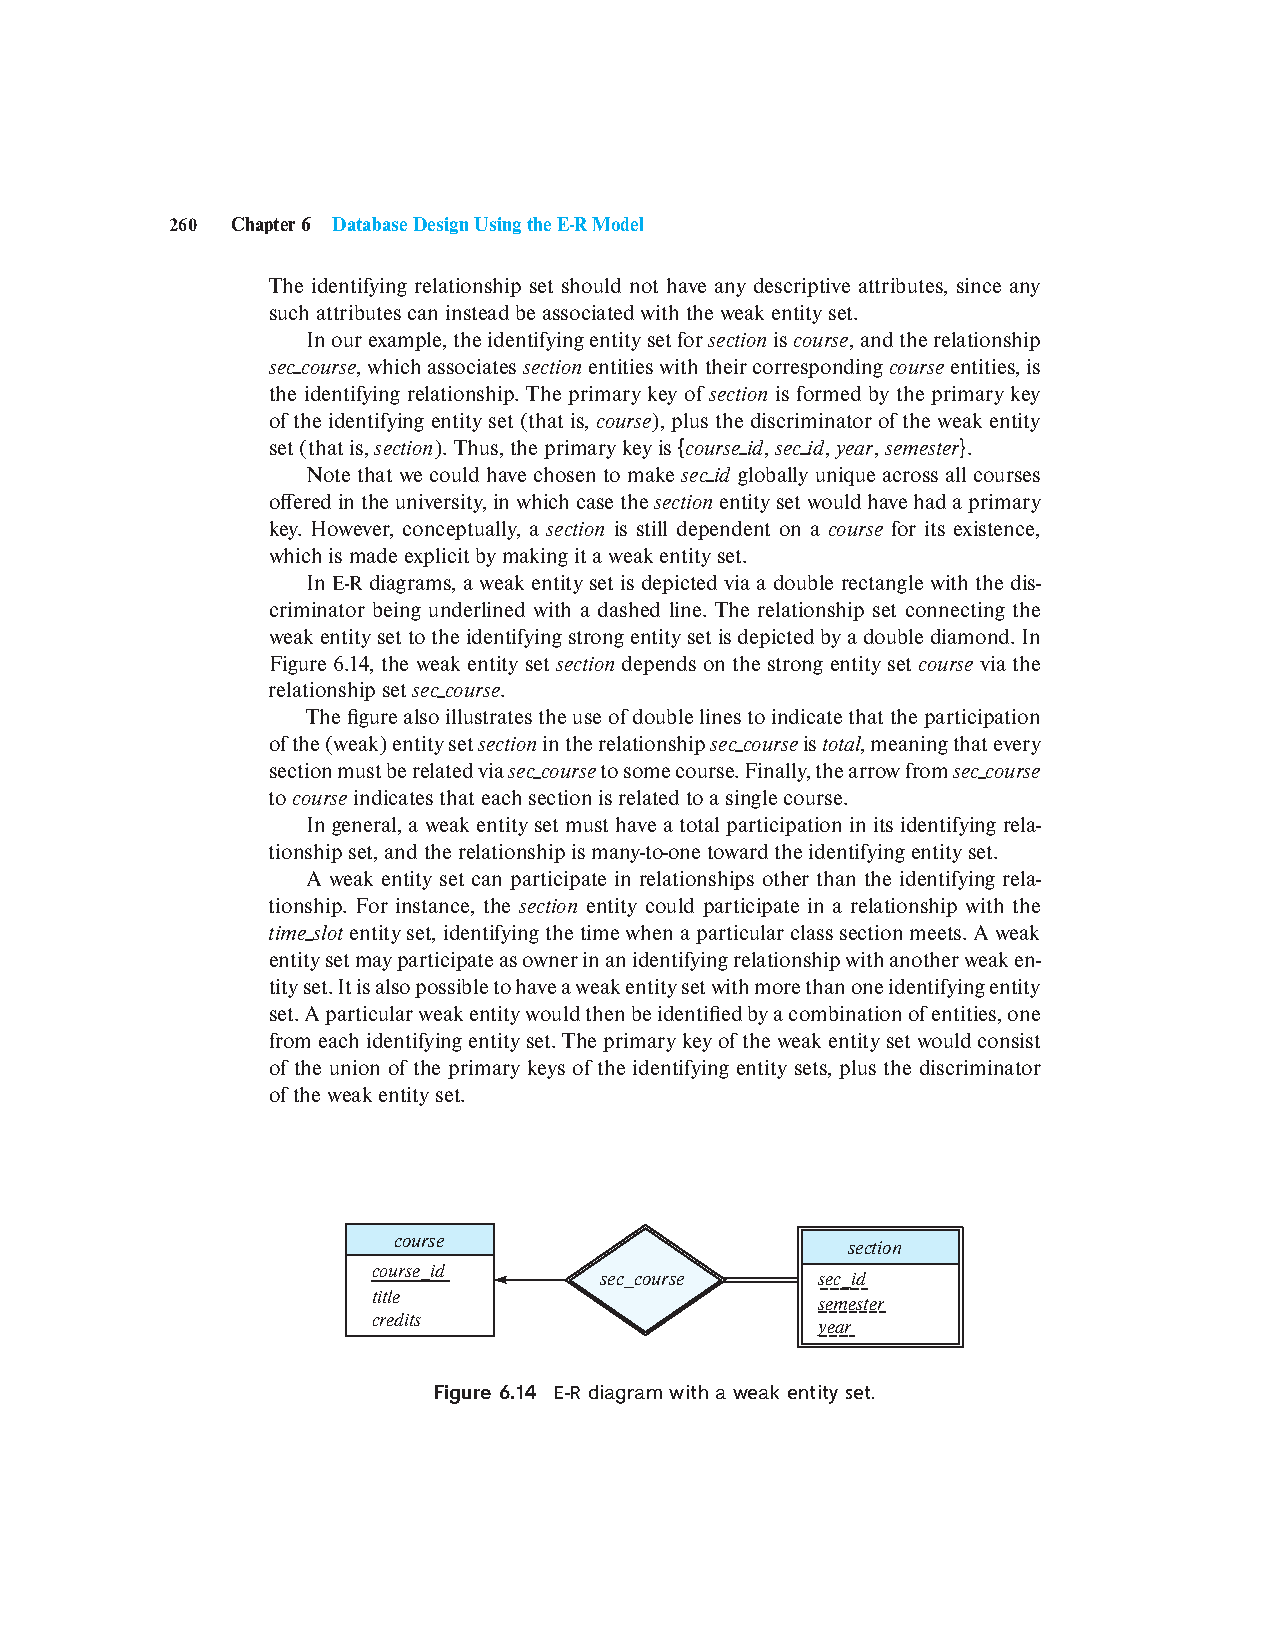
\includegraphics[trim={5cm 4.5cm 5cm 19.5cm}, clip, width=\textwidth]{figures/p260}
\end{frame}

\section{Removing Redundant Attributes in Entity Sets}

\begin{frame}{Redundant Attributes}
    \begin{itemize}
        \item Suppose we have entity sets:
        \begin{itemize}
            \item \texttt{student}, with attributes: ID, name, tot\_cred, dept\_name.
            \item \texttt{department}, with attributes: dept\_name, building, budget.
        \end{itemize}
        \item We model the fact that each student has an associated department using a relationship set \texttt{stud\_dept}.
        \item The attribute \texttt{dept\_name} in student below replicates information present in the relationship and is therefore redundant...
        \begin{itemize}
            \item and needs to be removed.
        \end{itemize}
        \item BUT: when converting back to tables, in some cases the attribute gets reintroduced, as we will see later.
    \end{itemize}
    \centering
    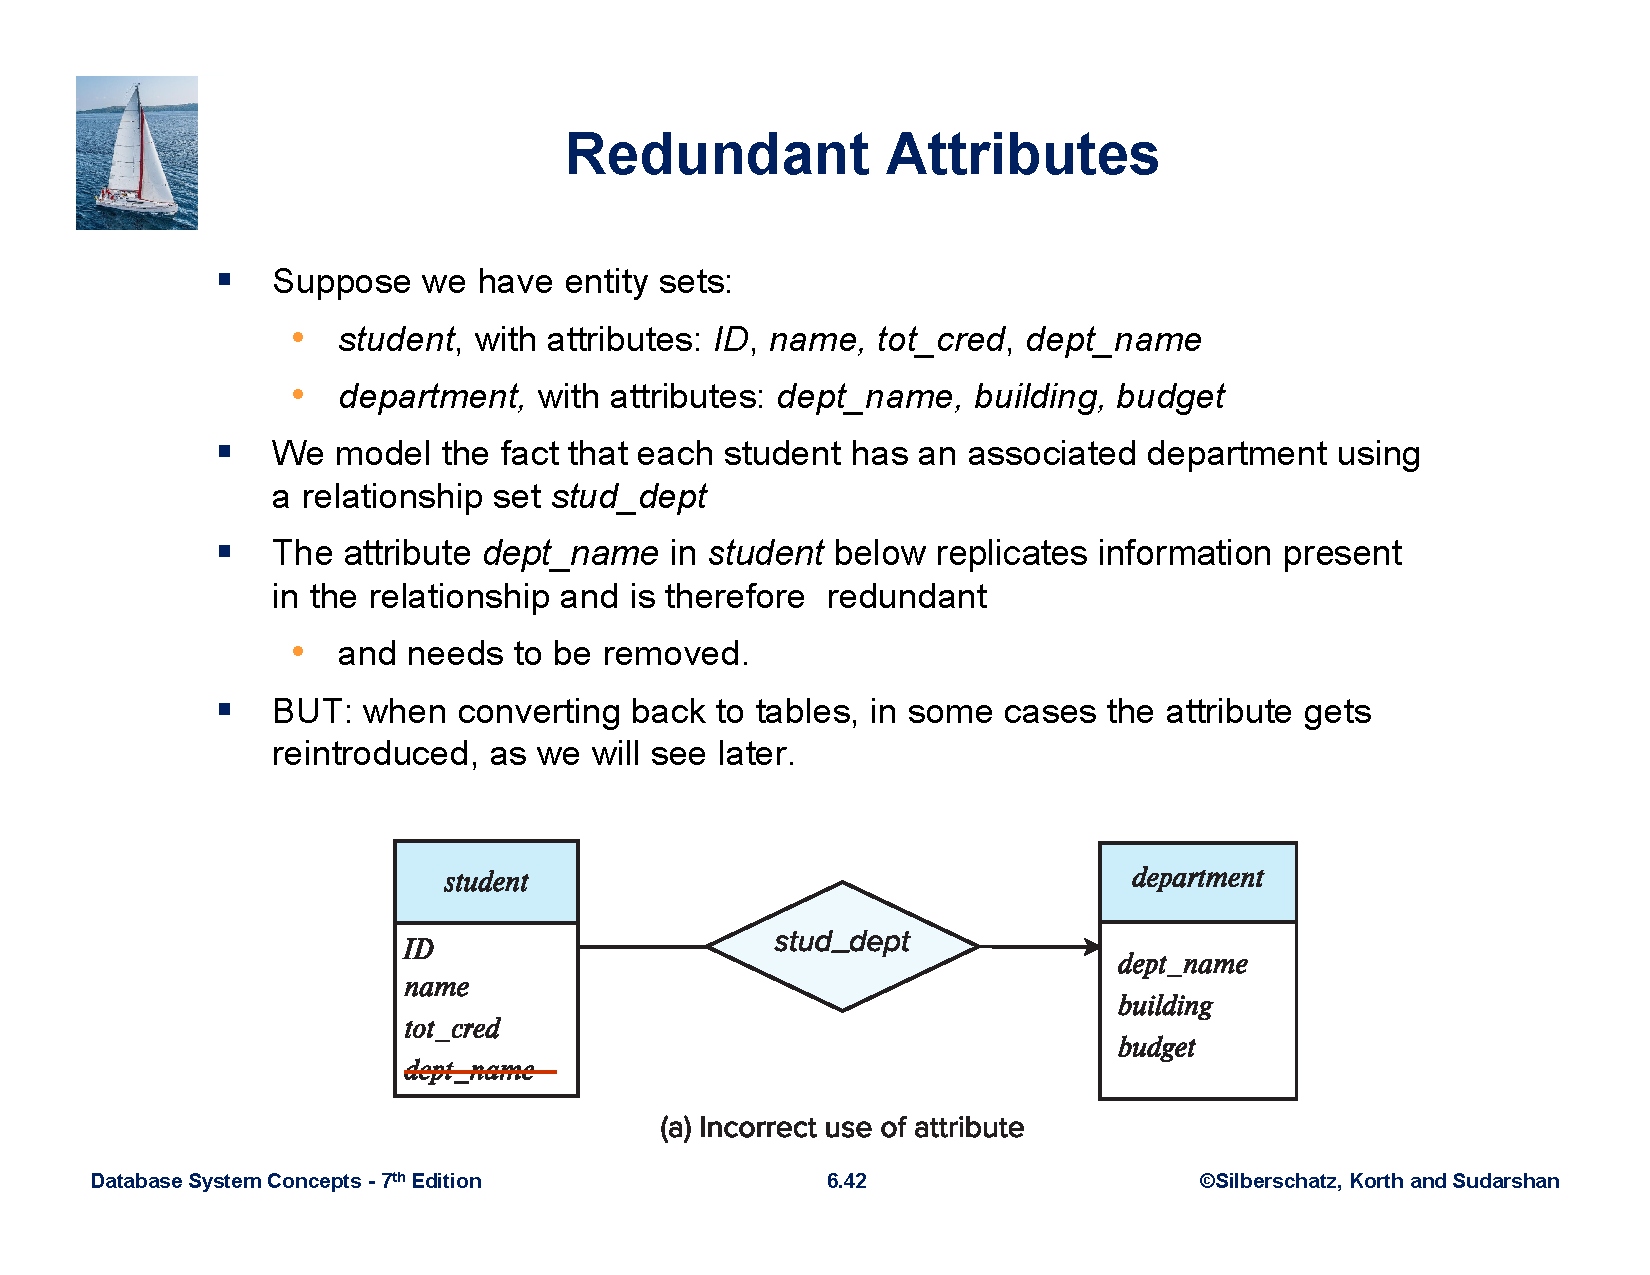
\includegraphics[trim={5cm 2cm 5cm 13.5cm}, clip, width=0.75\textwidth]{figures/redundant_attr}
\end{frame}

\begin{frame}{E-R Diagram for a University Enterprise}
    \centering
    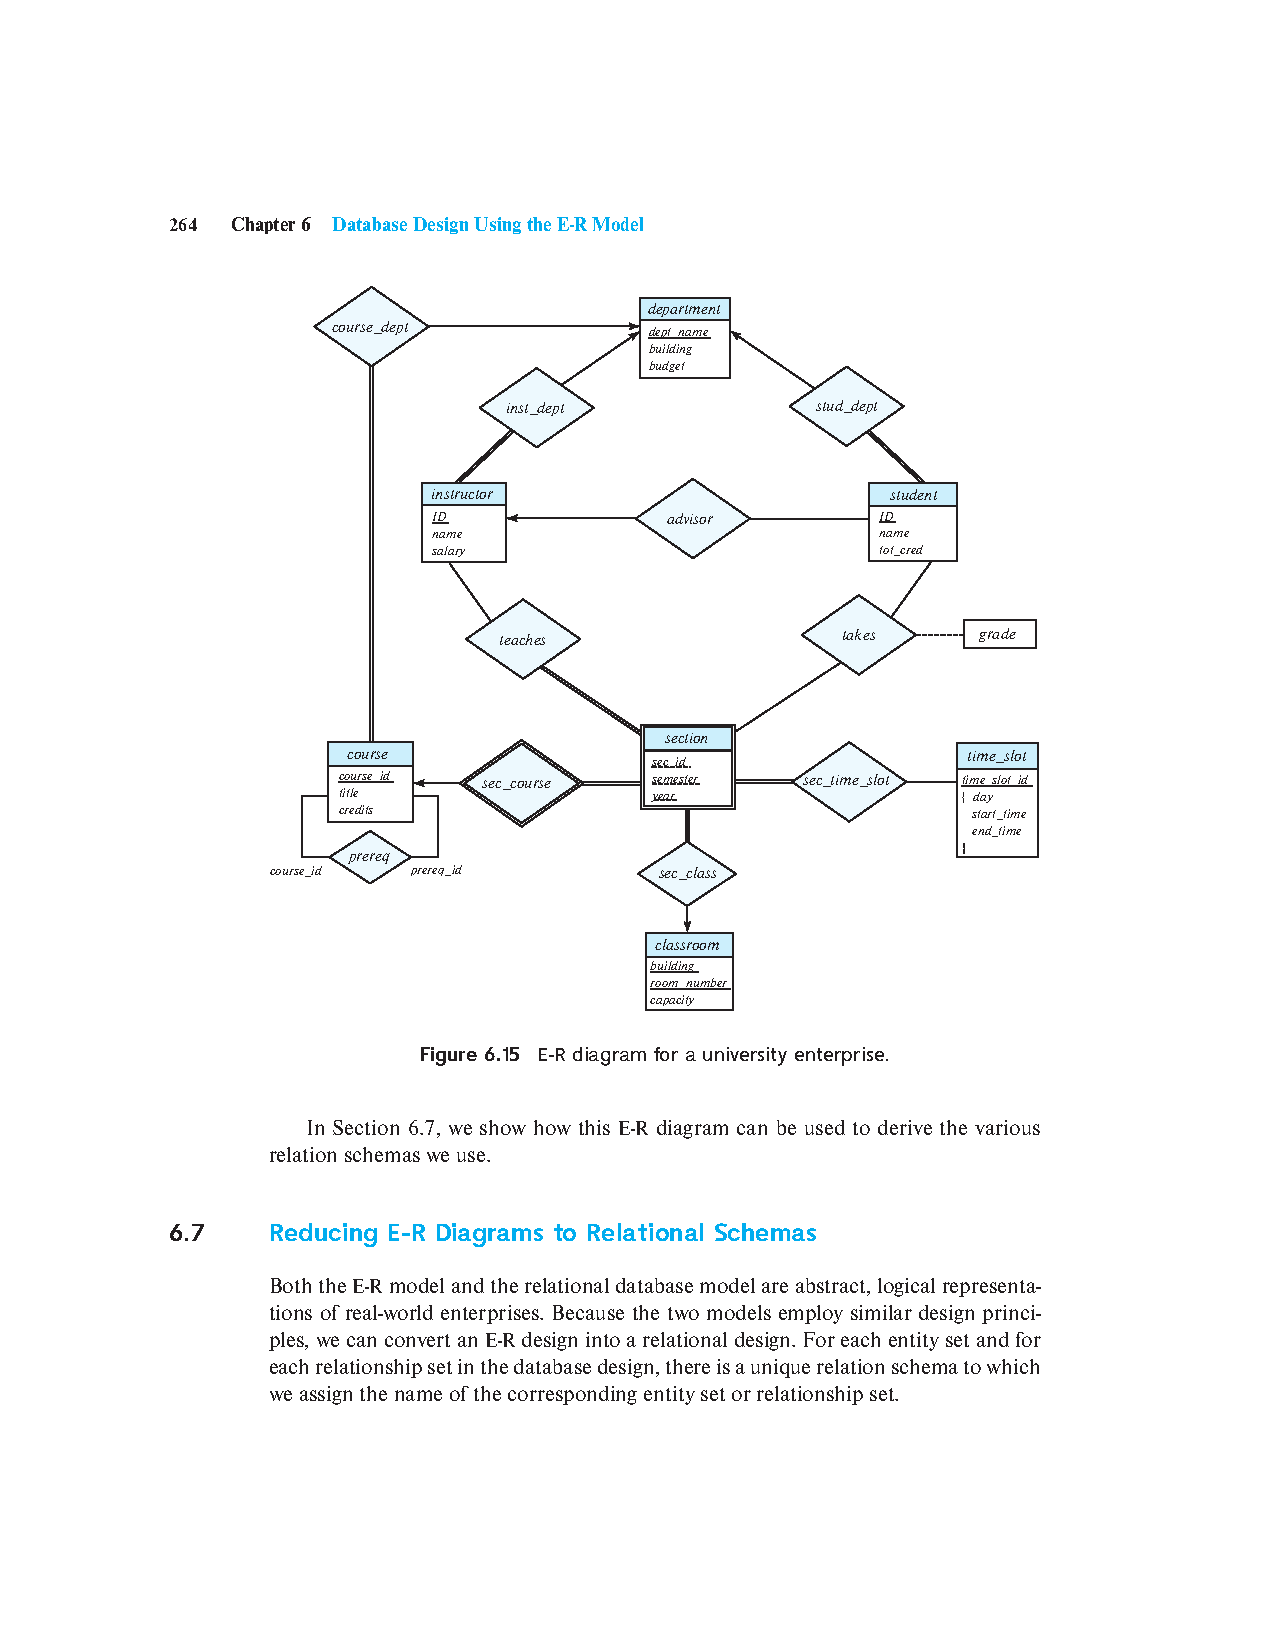
\includegraphics[trim={4.55cm 10.80cm 4.00cm 4.85cm}, clip, width=0.8\textwidth]{figures/p264}
\end{frame}

\section{Reducing E-R Diagrams to Relational Schemas}

\begin{frame}{Reduction to Relation Schemas}
    \begin{itemize}
        \item Entity sets and relationship sets can be expressed uniformly as relation schemas that represent the contents of the database.
        \item A database which conforms to an E-R diagram can be represented by a collection of schemas.
        \item For each entity set and relationship set there is a unique schema that is assigned the name of the corresponding entity set or relationship set.
        \item Each schema has a number of columns (generally corresponding to attributes), which have unique names.
    \end{itemize}
\end{frame}

\begin{frame}{Representing Entity Sets}
    \begin{itemize}
        \item A strong entity set reduces to a schema with the same attributes: \\
        \texttt{student(\underline{ID}, name, tot\_cred)}
        \item A weak entity set becomes a table that includes a column for the primary key of the identifying strong entity set: \\
        \texttt{section(\underline{course\_id}, \underline{sec\_id}, \underline{sem}, \underline{year})}
        \item Example:
        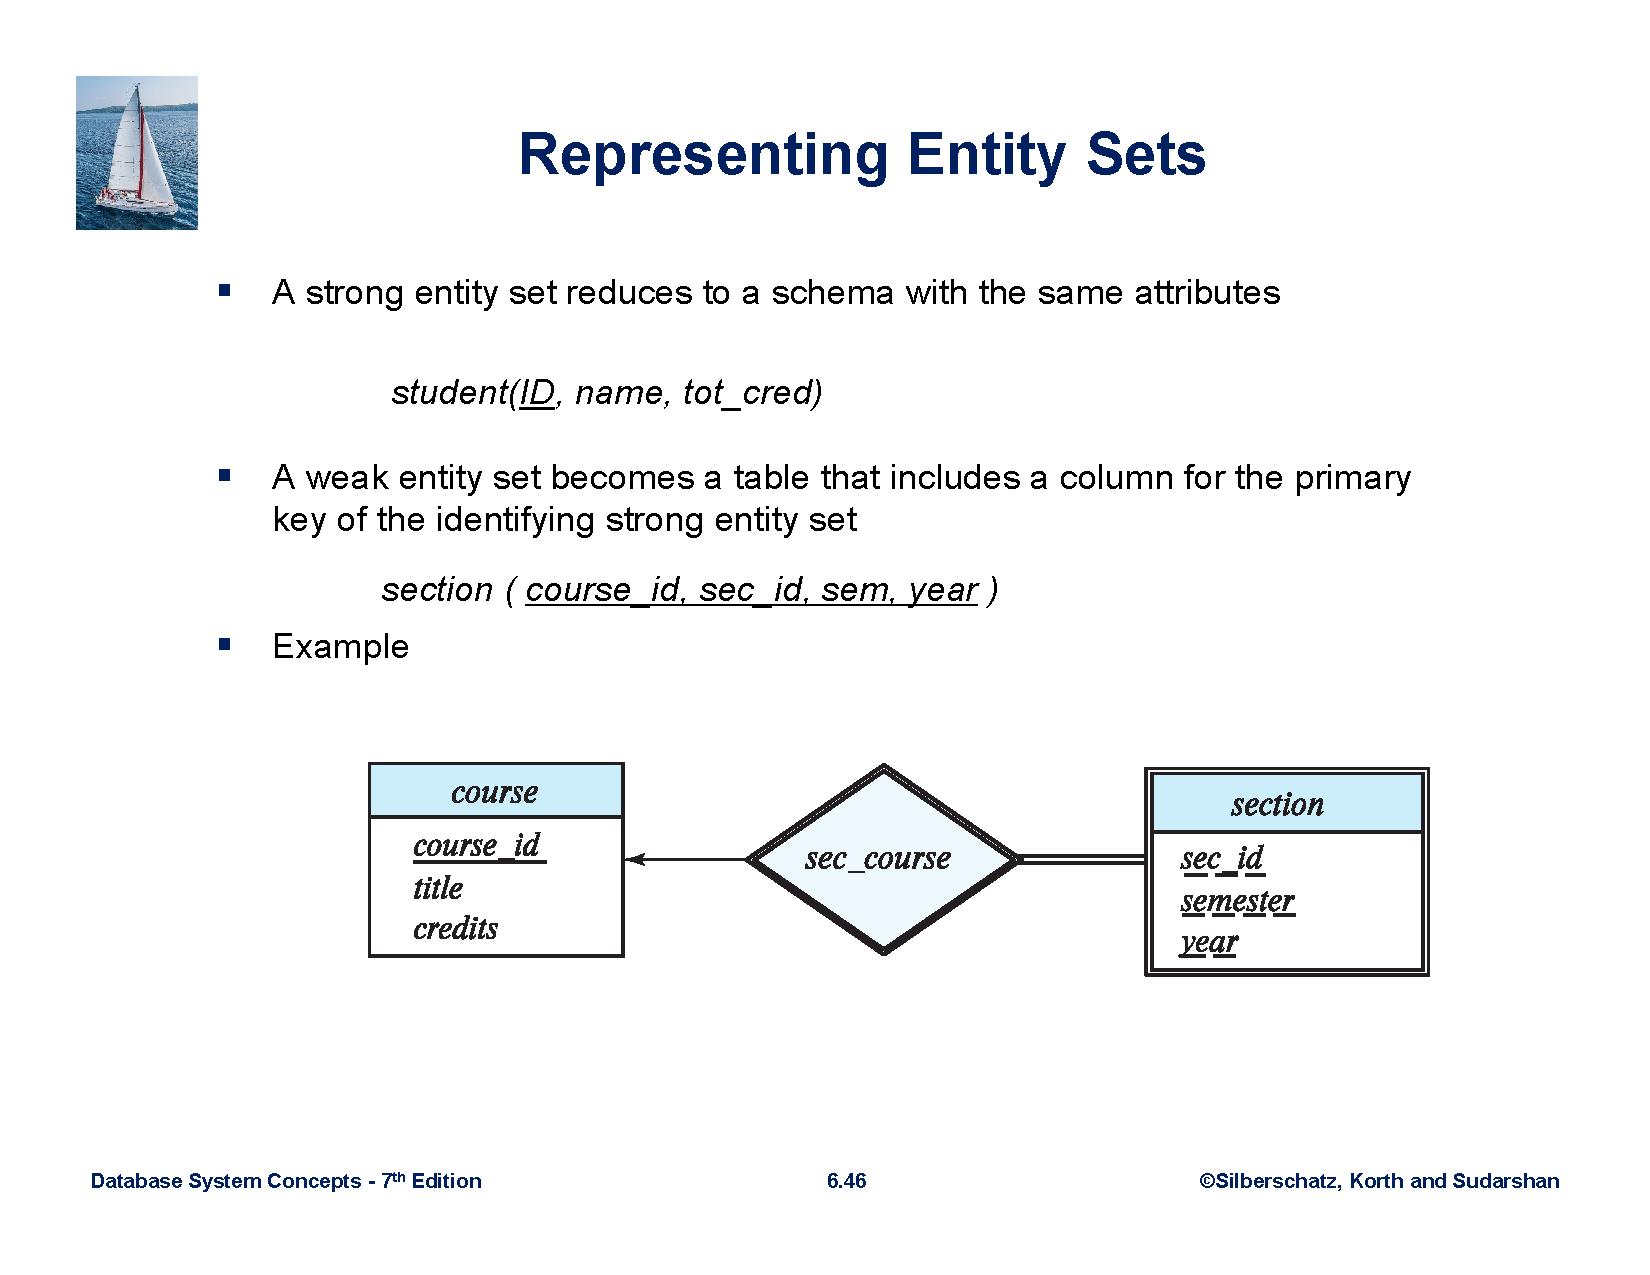
\includegraphics[width=\textwidth, clip,trim=0cm 5cm 0cm 12cm]{figures/weak_entities.pdf}
    \end{itemize}
\end{frame}

\begin{frame}{Representation of Entity Sets with Composite Attributes}
    \begin{minipage}{0.25\textwidth}
        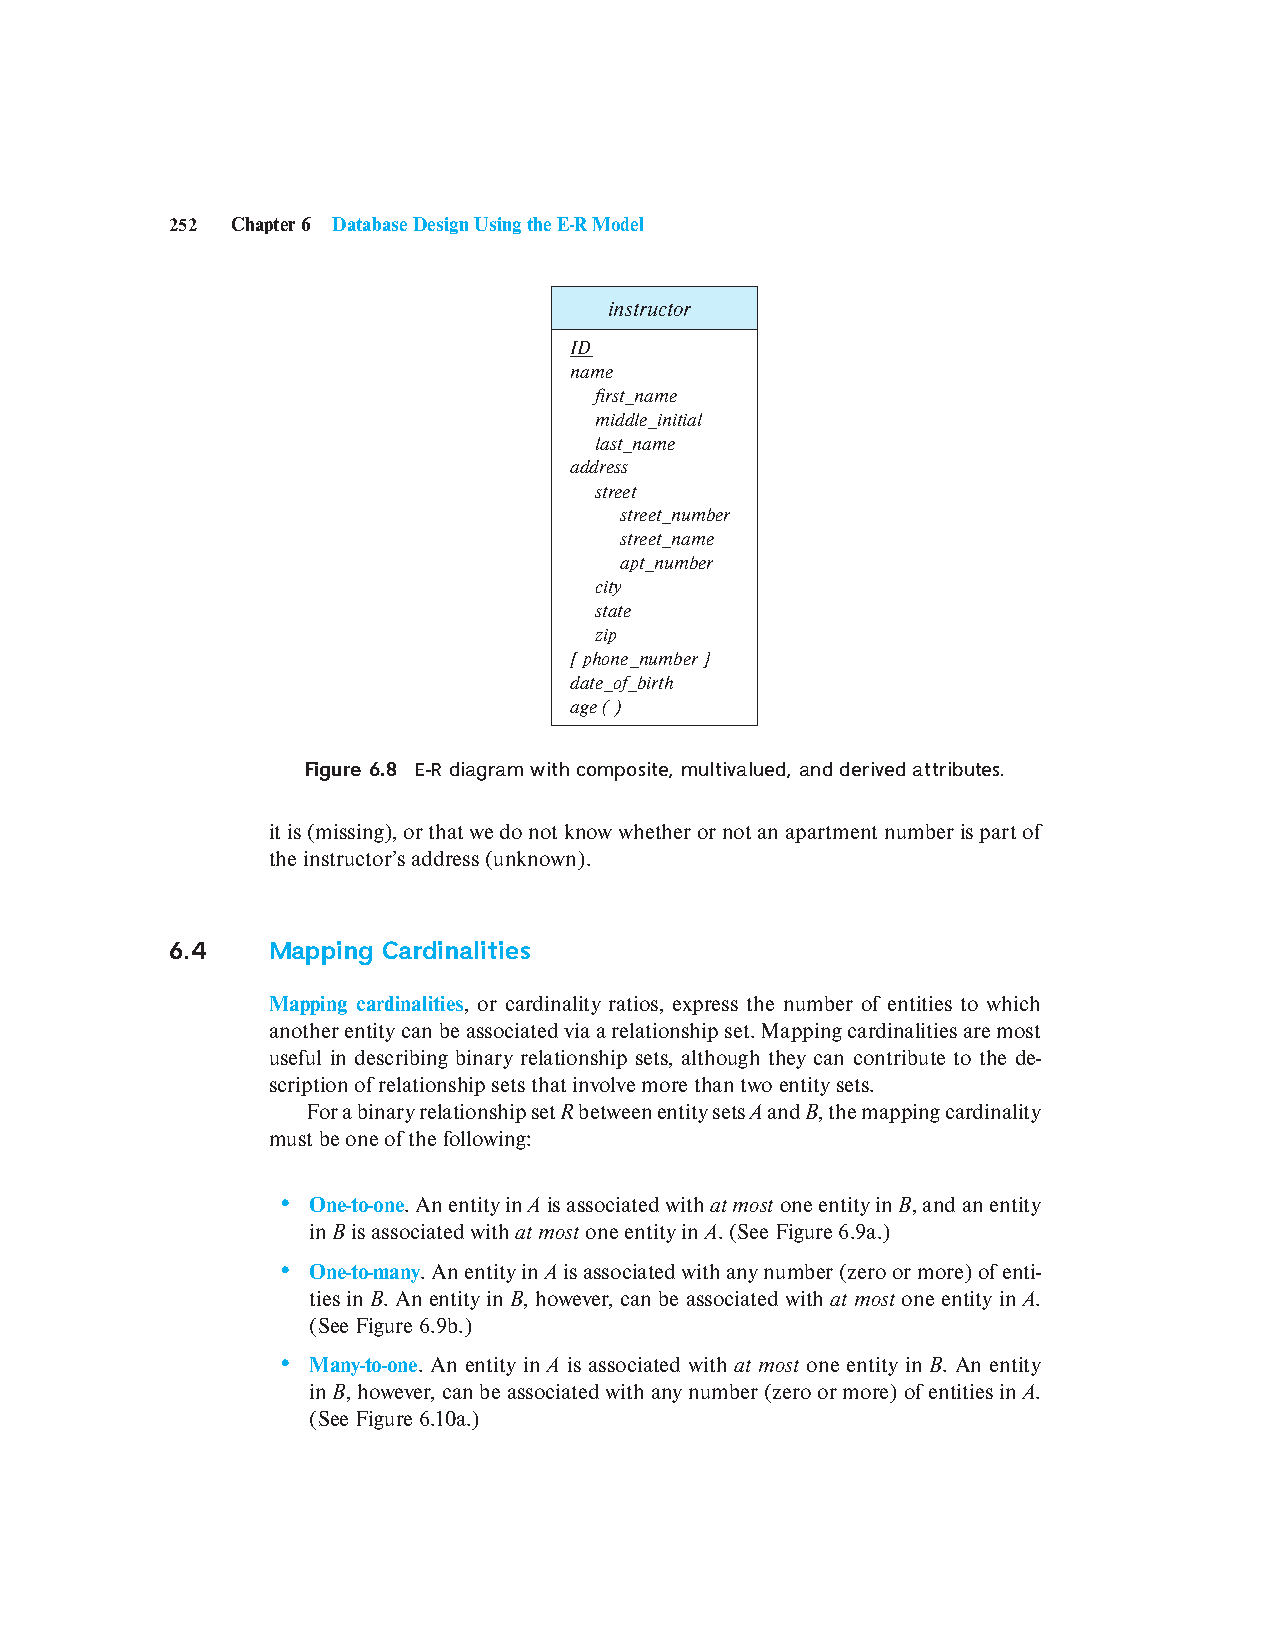
\includegraphics[trim={9.25cm 15.25cm 8.5cm 4cm}, clip, width=\textwidth]{figures/p252}
    \end{minipage}%
    \begin{minipage}{0.74\textwidth}
        \begin{itemize}
            \scriptsize
            \item Composite attributes are flattened out by creating a separate attribute for each component attribute.
            \begin{itemize}
                \scriptsize
                \item Example: given entity set \texttt{instructor} with composite attribute \texttt{name} with component attributes \texttt{first\_name} and \texttt{last\_name} the schema corresponding to the entity set has two attributes \texttt{name\_first\_name} and \texttt{name\_last\_name}.
                \begin{itemize}
                    \scriptsize
                    \item Prefix omitted if there is no ambiguity (\texttt{name\_first\_name} could be \texttt{first\_name})
                \end{itemize}
            \end{itemize}
            \item Ignoring multivalued attributes, extended \texttt{instructor} schema is:
            \begin{itemize}
                \scriptsize
                \item \texttt{instructor(ID, first\_name, middle\_initial, last\_name, street\_number, street\_name, apt\_number, city, state, zip\_code, date\_of\_birth)}
            \end{itemize}
        \end{itemize}
    \end{minipage}
\end{frame}

\begin{frame}{Representation of Entity Sets with Multivalued Attributes}
    \begin{itemize}
        \item A multivalued attribute \textit{M} of an entity \textit{E} is represented by a separate schema \textit{EM}.
        \item Schema \textit{EM} has attributes corresponding to the primary key of \textit{E} and an attribute corresponding to multivalued attribute \textit{M}.
        \item Example: Multivalued attribute \texttt{phone\_number} of \texttt{instructor} is represented by a schema: \\
        \texttt{inst\_phone = (\underline{ID}, \underline{phone\_number})}.
        \item Each value of the multivalued attribute maps to a separate tuple of the relation on schema \textit{EM}:
        \begin{itemize}
            \item For example, an instructor entity with primary key 22222 and phone numbers 456-7890 and 123-4567 maps to two tuples: (22222, 456-7890) and (22222, 123-4567)
        \end{itemize}
    \end{itemize}
\end{frame}

\begin{frame}{Representing Relationship Sets}
    \begin{itemize}
        \item A many-to-many relationship set is represented as a schema with attributes for the primary keys of the two participating entity sets, and any descriptive attributes of the relationship set.
        \item Example: schema for relationship set advisor. \\
        \texttt{advisor = (\underline{s\_id}, \underline{i\_id})}
    \end{itemize}
    \centering
    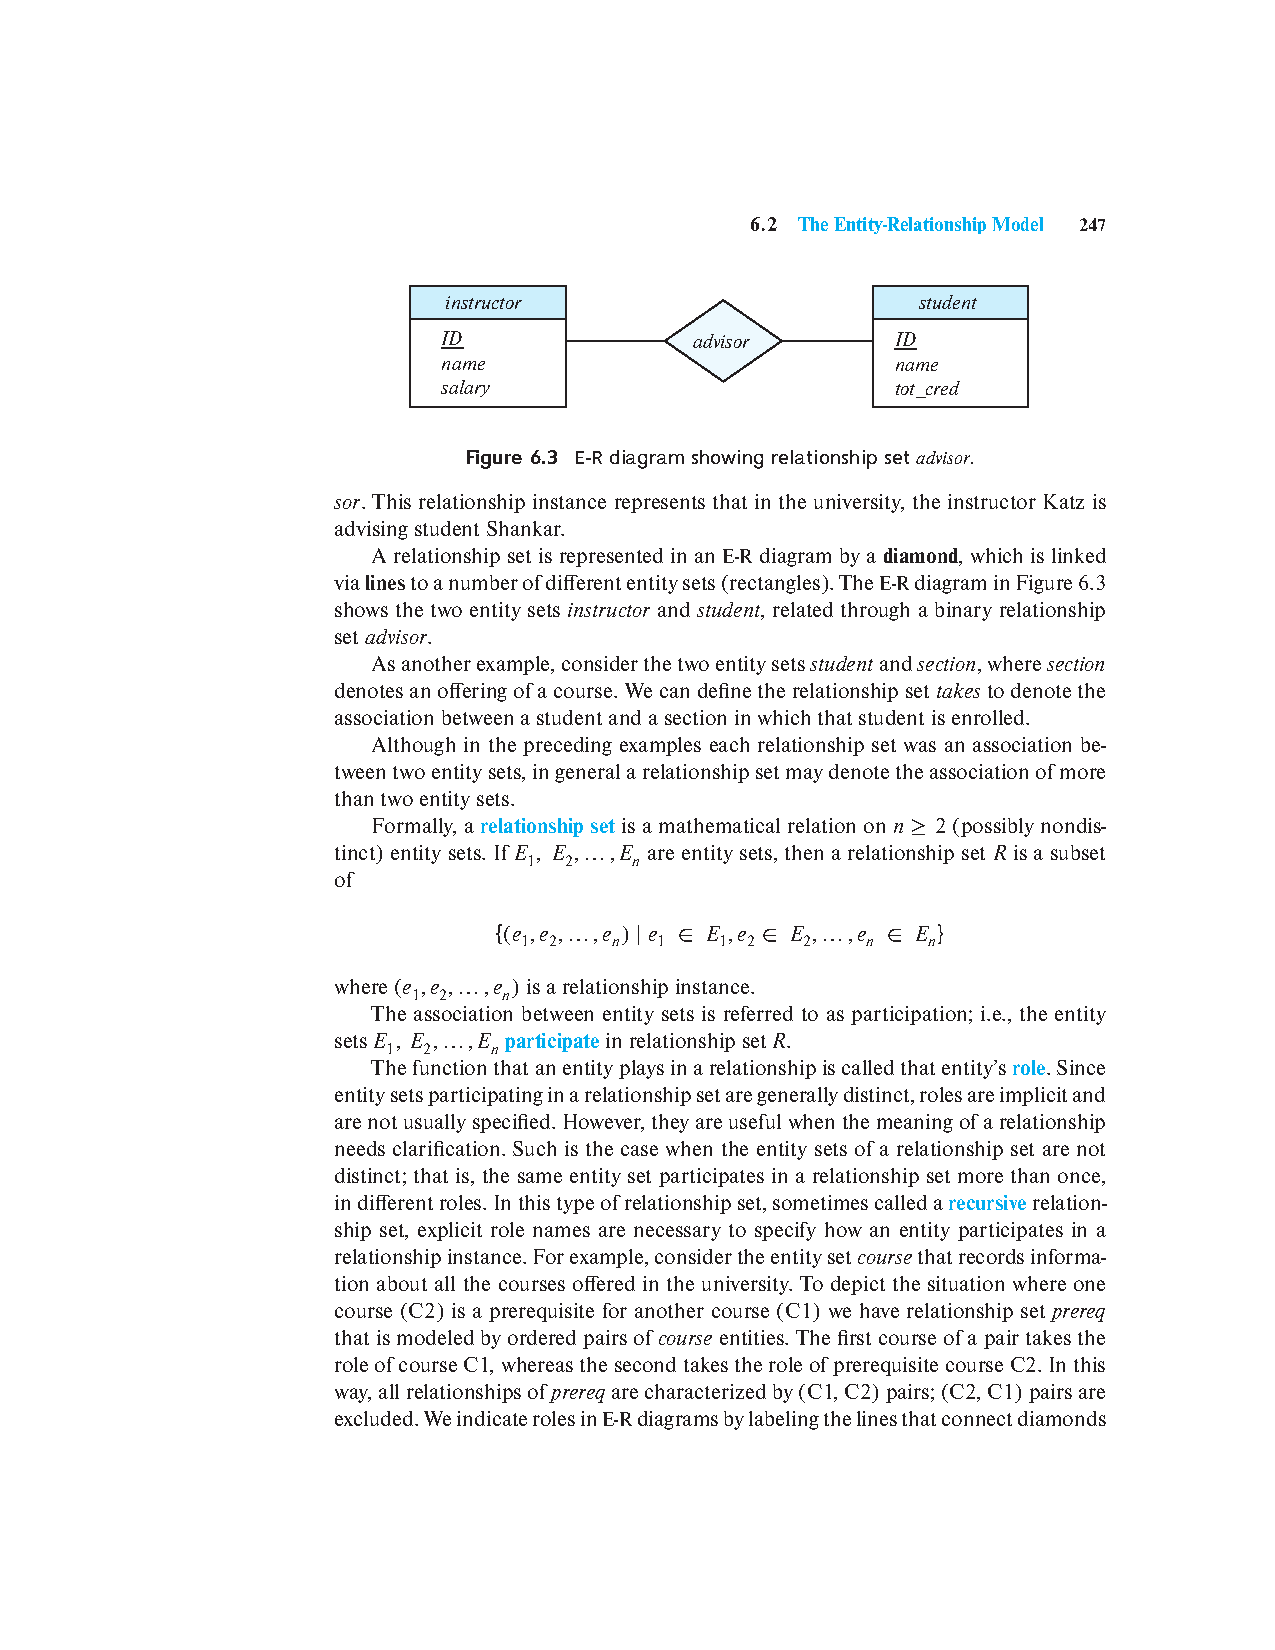
\includegraphics[trim={6.90cm 21cm 4.15cm 4cm}, clip, width=\textwidth]{figures/p247}
\end{frame}

\begin{frame}{Redundancy of Schemas}
    \begin{itemize}
        \item Many-to-one and one-to-many relationship sets that are total on the many-side can be represented by adding an extra attribute to the ``many'' side, containing the primary key of the ``one'' side.
        \item Example: Instead of creating a schema for relationship set \texttt{inst\_dept}, add an attribute \textit{dept\_name} to the schema arising from entity set \texttt{instructor}.
    \end{itemize}
    \centering
    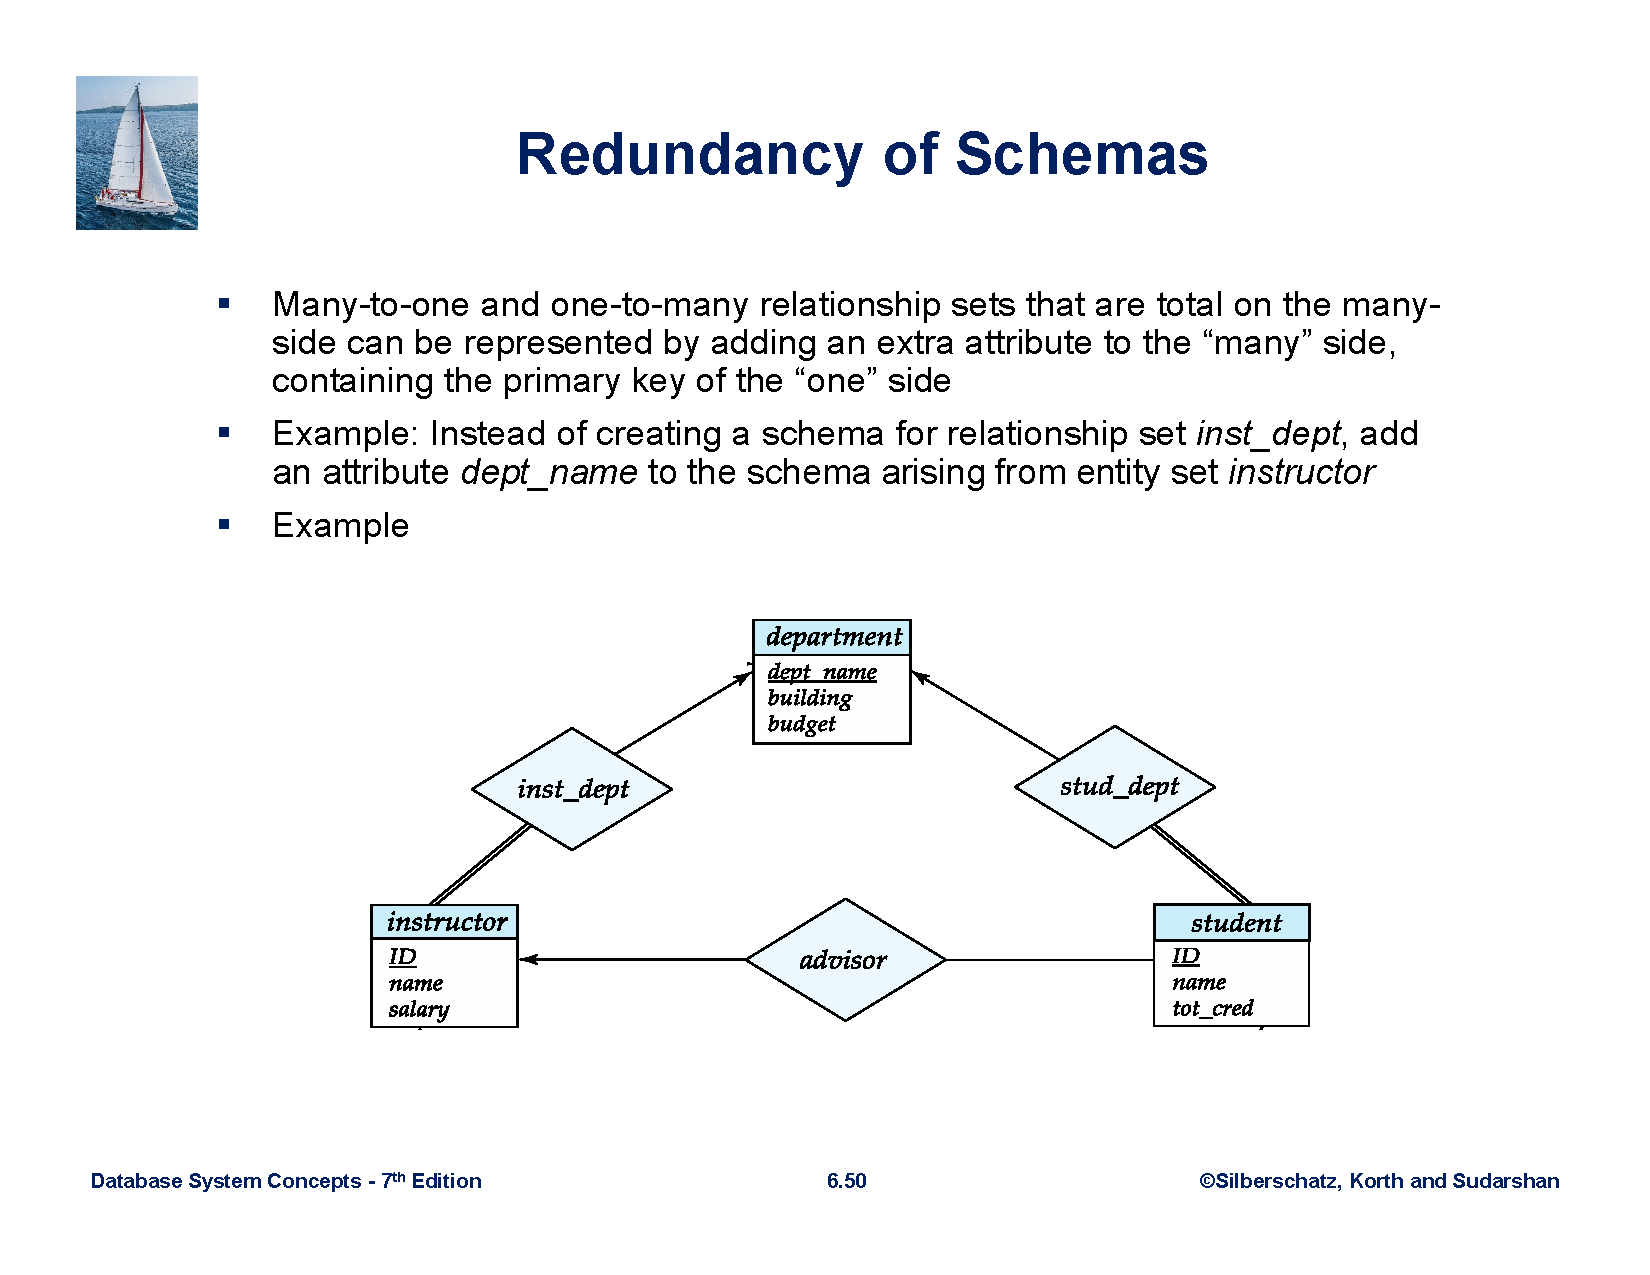
\includegraphics[trim={2cm 4cm 2cm 10cm}, clip, width=\textwidth]{figures/redundancy}
\end{frame}

\begin{frame}{Redundancy of Schemas (Cont.)}
    \begin{itemize}
        \item For one-to-one relationship sets, either side can be chosen to act as the ``many'' side:
        \begin{itemize}
            \item That is, an extra attribute can be added to either of the tables corresponding to the two entity sets.
        \end{itemize}
        \item If participation is partial on the ``many'' side, replacing a schema by an extra attribute in the schema corresponding to the ``many'' side could result in \texttt{\textbf{null}} values.
    \end{itemize}
\end{frame}

\begin{frame}{Redundancy of Schemas (Cont.)}
    \begin{itemize}
        \item The schema corresponding to a relationship set linking a weak entity set to its identifying strong entity set is redundant.
        \item Example: The \texttt{section} schema already contains the attributes that would appear in the \texttt{sec\_course} schema.
    \end{itemize}
    \centering
    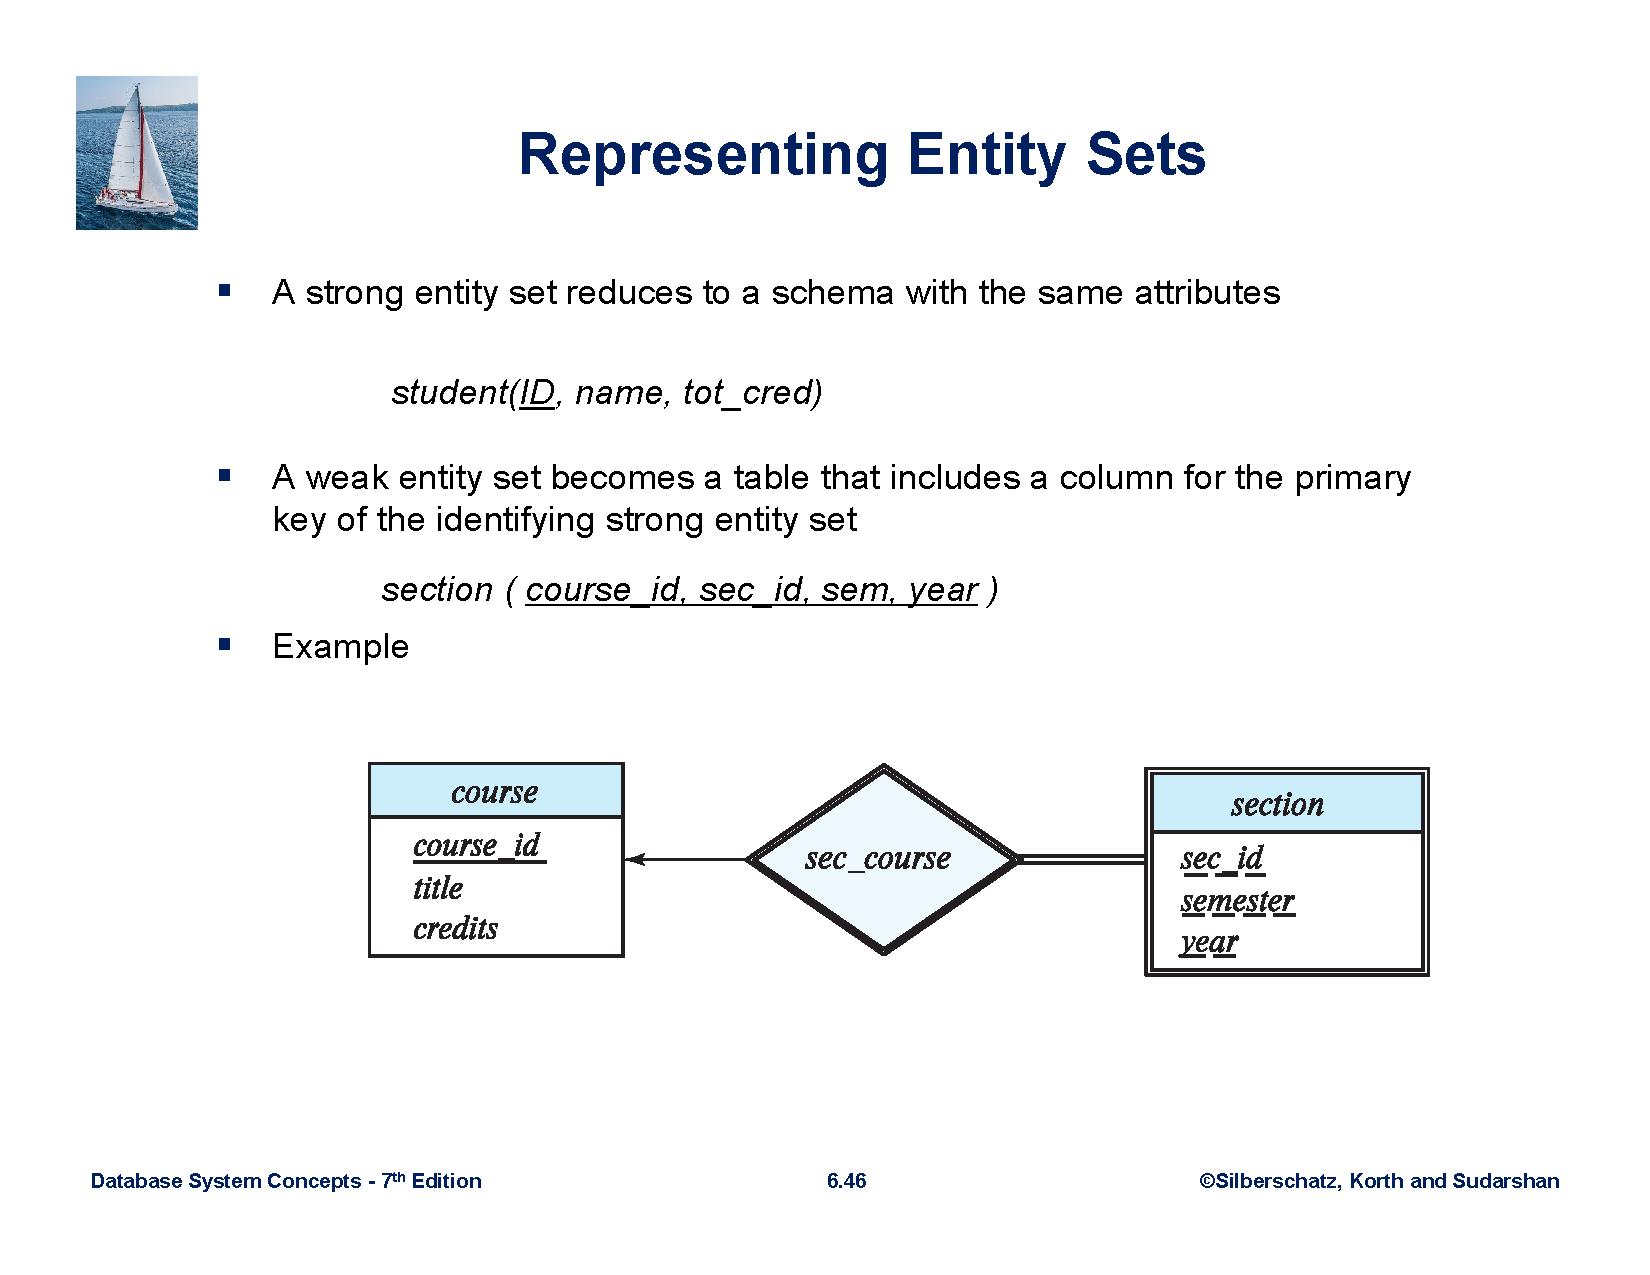
\includegraphics[trim={5cm 5cm 3cm 12cm}, clip, width=\textwidth]{figures/weak_entities}
\end{frame}

\section{Extended E-R Features}

\begin{frame}{Specialization}
    \begin{itemize}
        \item Top-down design process; we designate sub-groupings within an entity set that are distinctive from other entities in the set.
        \item These sub-groupings become lower-level entity sets that have attributes or participate in relationships that do not apply to the higher-level entity set.
        \item Depicted by a triangle component labeled ISA (e.g., \texttt{instructor} ``is a'' \texttt{person}).
        \item \textbf{Attribute inheritance} – a lower-level entity set inherits all the attributes and relationship participation of the higher-level entity set to which it is linked.
    \end{itemize}
\end{frame}

\begin{frame}{Specialization Example}
    \begin{itemize}
        \item Overlapping – employee and student.
        \item Disjoint – instructor and secretary.
        \item Total and partial.
    \end{itemize}
    \centering
    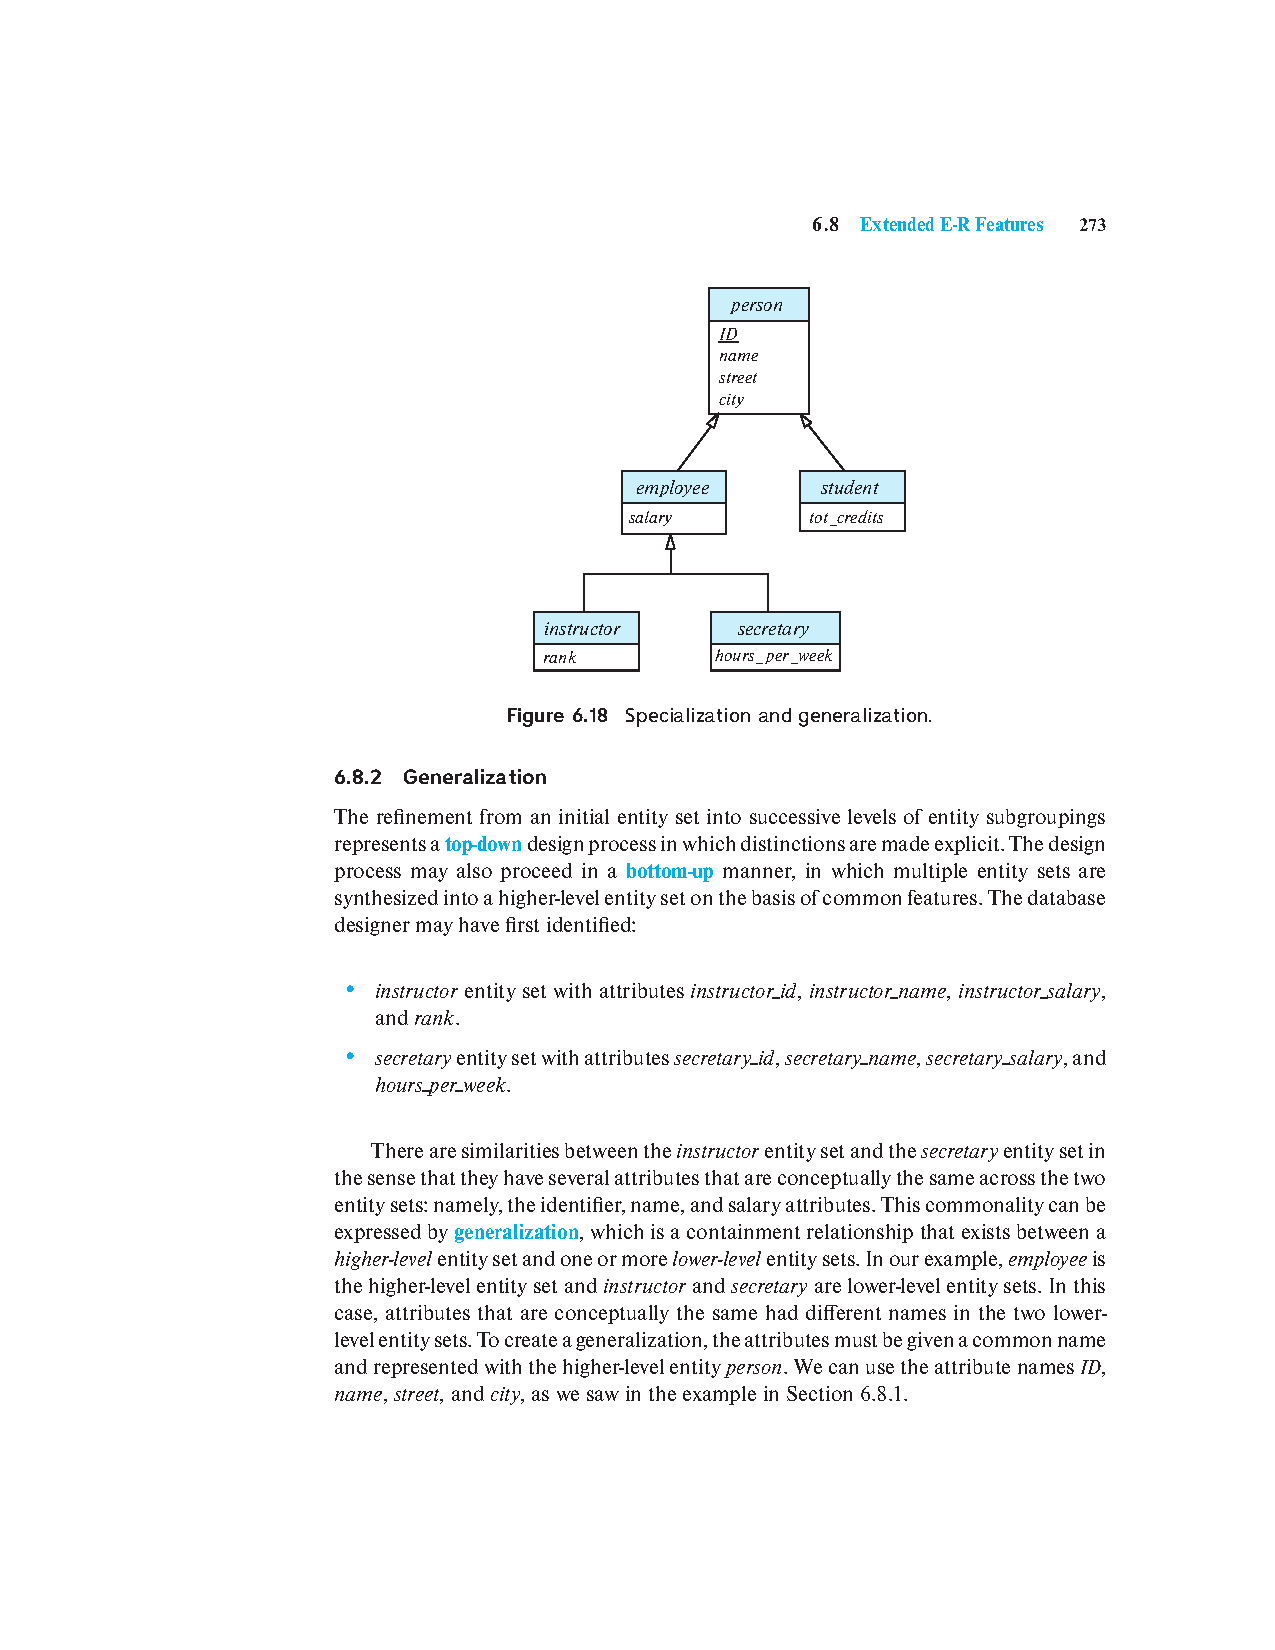
\includegraphics[trim={6cm 16cm 4cm 4.8cm}, clip, width=\textwidth]{figures/specialization}
\end{frame}

\begin{frame}{Representing Specialization via Schemas}
    \begin{itemize}
        \item Method 1:
        \begin{itemize}
            \item Form a schema for the higher-level entity.
            \item Form a schema for each lower-level entity set, include primary key of higher-level entity set and local attributes.\\
            \vspace{3mm}
            \begin{tabular}{l | l}
                Schema & Attributes \\ \hline
                person      & ID, name, stree, city \\
                student     & ID, tot\_cred \\
                employee    & ID, salary \\
            \end{tabular}
            \bigskip
            \item Drawback: getting information about, an employee requires accessing two relations, the one corresponding to the low-level schema and the one corresponding to the high-level schema.
        \end{itemize}
    \end{itemize}
\end{frame}

\begin{frame}{Representing Specialization via Schemas}
    \begin{itemize}
        \item Method 2:
        \begin{itemize}
            \item Form a schema for each entity set with all local and inherited attributes.\\
            \vspace{3mm}
            \begin{tabular}{l | l}
                Schema & Attributes \\ \hline
                person      & ID, name, stree, city \\
                student     & ID, name, stree, city, tot\_cred \\
                employee    & ID, name, stree, city, salary \\
            \end{tabular}
            \bigskip
            \item Drawback: \textit{name}, \textit{street} and \textit{city} may be stored redundantly for people who are both students and employees.
        \end{itemize}
    \end{itemize}
\end{frame}

\begin{frame}{Generalization}
    \begin{itemize}
        \item \textbf{A bottom-up design process} – combine a number of entity sets that share the same features into a higher-level entity set.
        \item Specialization and generalization are simple inversions of each other; they are represented in an E-R diagram in the same way.
        \item The terms specialization and generalization are used interchangeably.
    \end{itemize}
\end{frame}

\begin{frame}{Completeness constraint}
    \begin{itemize}
        \item Completeness constraint -- specifies whether or not an entity in the higher-level entity set must belong to at least one of the lower-level entity sets within a generalization.
        \begin{itemize}
            \item total: an entity must belong to one of the lower-level entity sets.
            \item partial: an entity need not belong to one of the lower-level entity sets.
        \end{itemize}
    \end{itemize}
\end{frame}

\begin{frame}{Completeness constraint (Cont.)}
    \begin{itemize}
        \item Partial generalization is the default.
        \item We can specify total generalization in an E-R diagram by adding the keyword \textbf{total} in the diagram and drawing a dashed line from the keyword to the corresponding hollow arrow-head to which it applies (for a total generalization), or to the set of hollow arrow-heads to which it applies (for an overlapping generalization).
        \item The \texttt{student} generalization is total: All student entities must be either graduate or undergraduate. Because the higher-level entity set arrived at through generalization is generally composed of only those entities in the lower-level entity sets, the completeness constraint for a generalized higher-level entity set is usually total.
    \end{itemize}
\end{frame}

\begin{frame}{Aggregation}
    \begin{itemize}
        \item Consider the ternary relationship \textit{proj\_guide}, which we saw earlier.
        \item Suppose we want to record evaluations of a student by a guide on a project.
    \end{itemize}
    \centering
    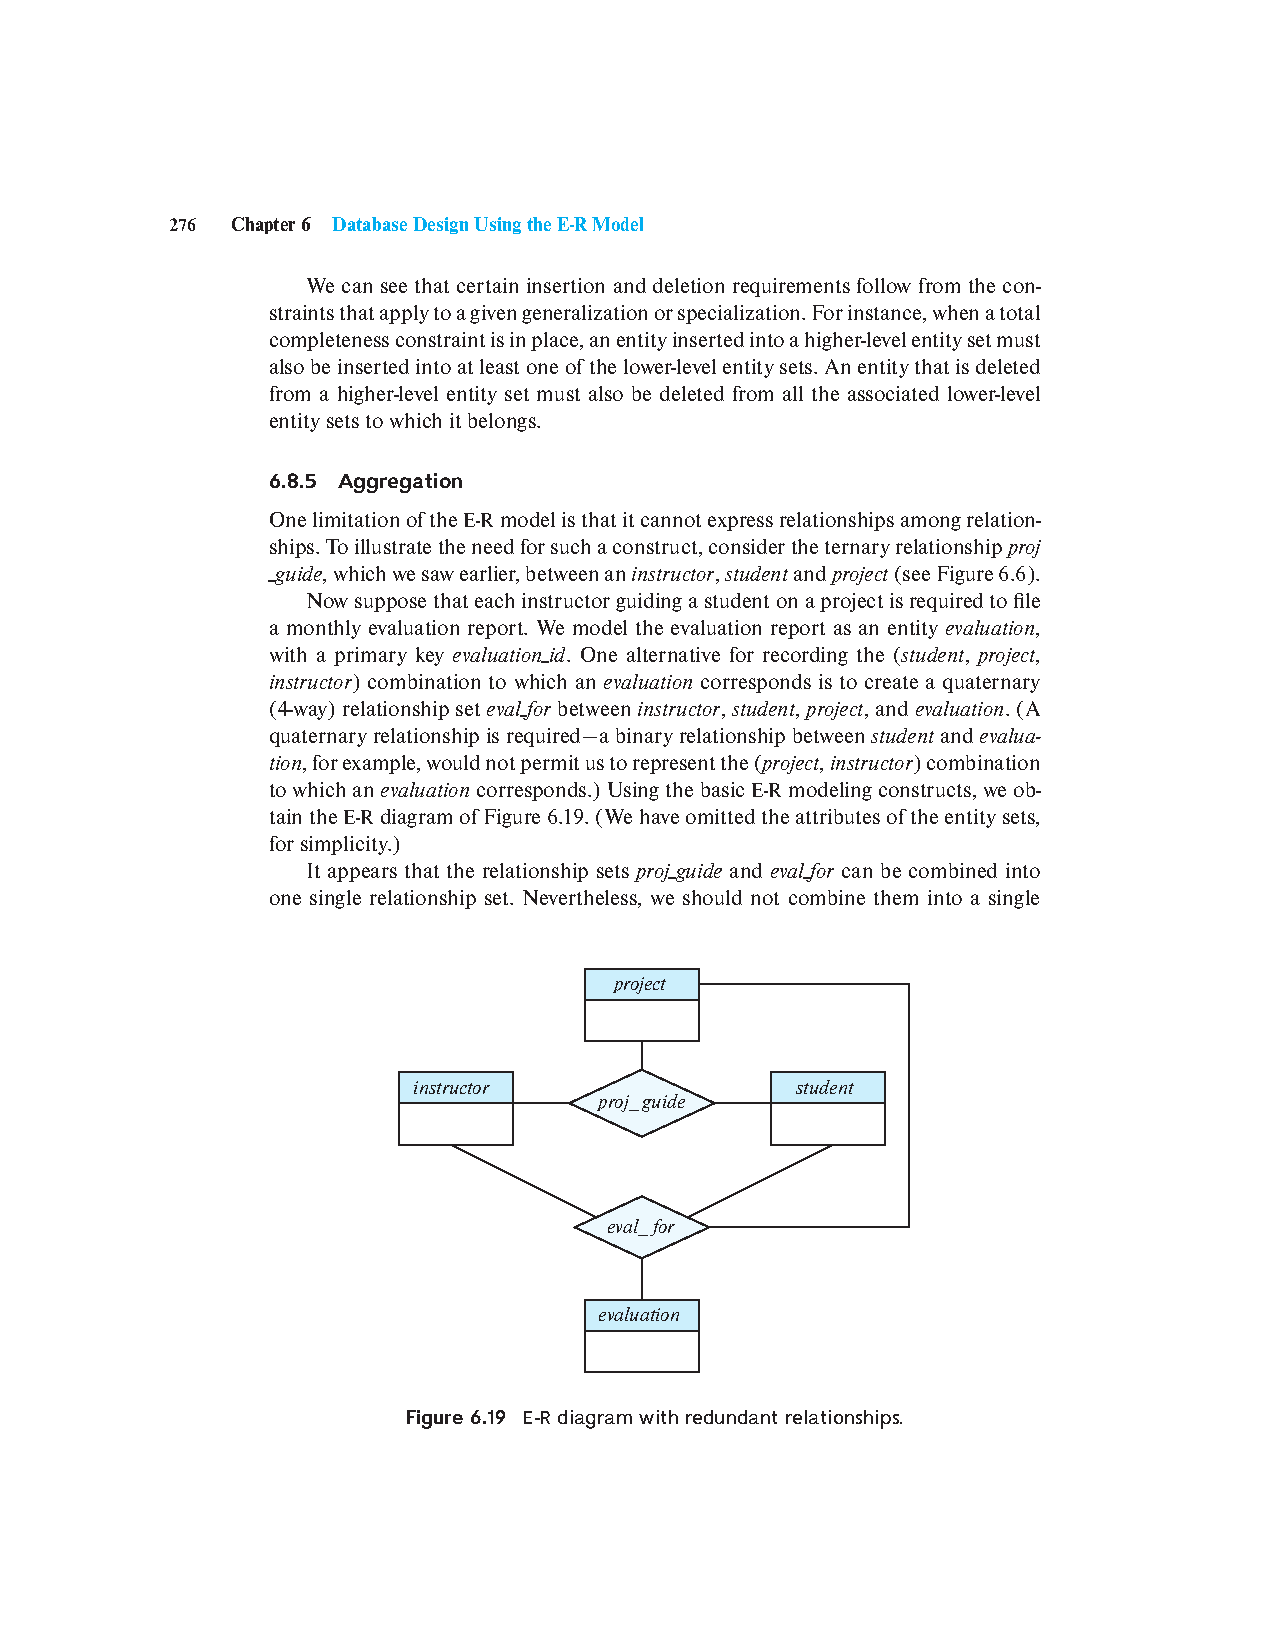
\includegraphics[trim={4cm 4.25cm 4cm 16cm}, clip, width=\textwidth]{figures/redundat_relationships}
\end{frame}

\begin{frame}{Aggregation (Cont.)}
    \begin{itemize}
        \item Relationship sets \textit{eval\_for} and \textit{proj\_guide} represent overlapping information:
        \begin{itemize}
            \item Every \textit{eval\_for} relationship corresponds to a \textit{proj\_guide} relationship.
            \item However, some \textit{proj\_guide} relationships may not correspond to any \textit{eval\_for} relationships.
            \begin{itemize}
                \item So we can't discard the \textit{proj\_guide} relationship.
            \end{itemize}
        \end{itemize}
        \item Eliminate this redundancy via aggregation:
        \begin{itemize}
            \item Treat relationship as an abstract entity.
            \item Allows relationships between relationships.
            \item Abstraction of relationship into new entity.
        \end{itemize}
    \end{itemize}
\end{frame}

\begin{frame}{Aggregation (Cont.)}
    \begin{itemize}
        \item Eliminate this redundancy via \textbf{aggregation} without introducing redundancy, the following diagram represents:
        \begin{itemize}
            \item A student is guided by a particular instructor on a particular project.
            \item A student, instructor, project combination may have an associated evaluation.
        \end{itemize}
    \end{itemize}
    \centering
    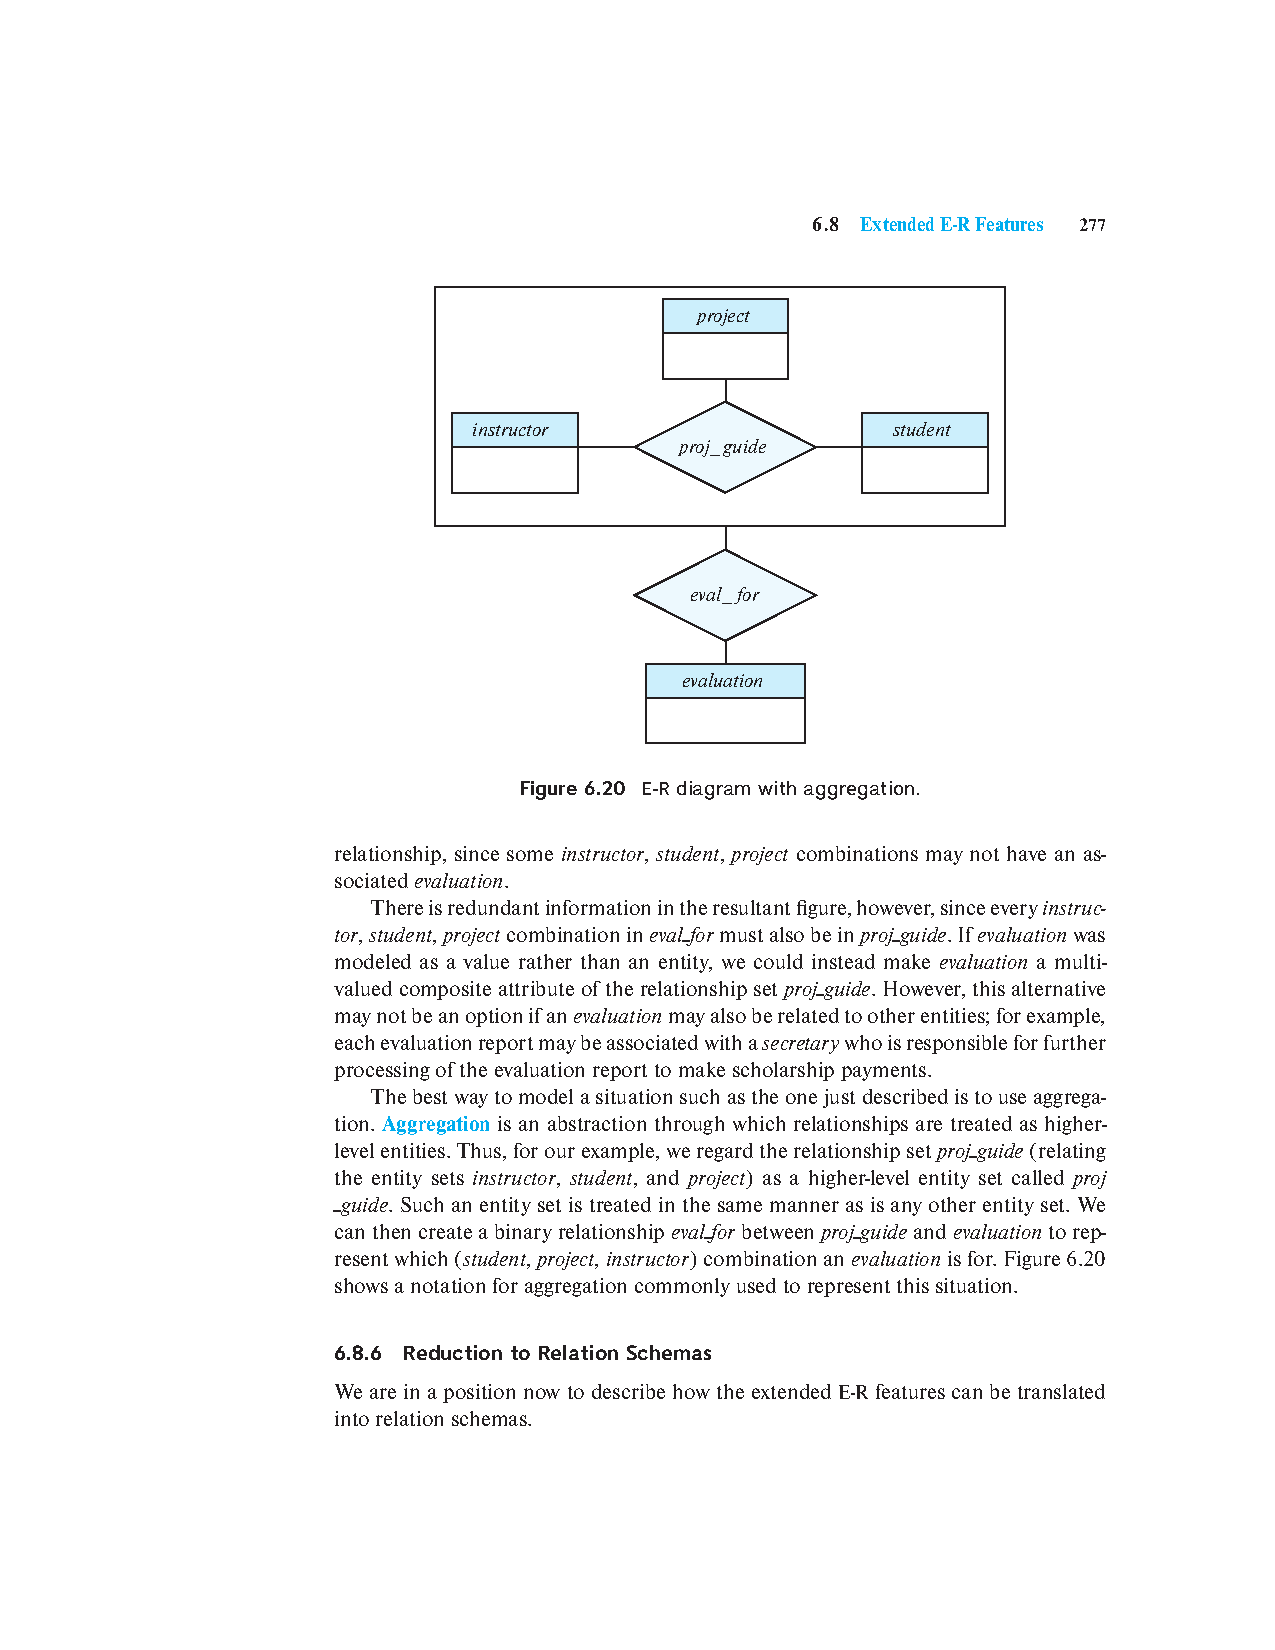
\includegraphics[trim={2cm 15cm 2cm 4cm}, clip, width=\textwidth]{figures/aggregation_relationships}
\end{frame}

\begin{frame}{Reduction to Relational Schemas}
    \begin{itemize}
        \item To represent aggregation, create a schema containing:
        \begin{itemize}
            \item Primary key of the aggregated relationship,
            \item The primary key of the associated entity set,
            \item Any descriptive attributes.
        \end{itemize}
        \item In our example:
        \begin{itemize}
            \item The schema \texttt{eval\_for} is: \\
                \texttt{eval\_for(s\_ID, project\_id, i\_ID, evaluation\_id)}
            \item The schema \texttt{proj\_guide} is redundant.
        \end{itemize}
    \end{itemize}
\end{frame}

\section{Entity-Relationship Design Issues}

\begin{frame}{Common Mistakes in E-R Diagrams}
    \begin{itemize}
        \item Example of erroneous E-R diagrams:
    \end{itemize}
    \centering
    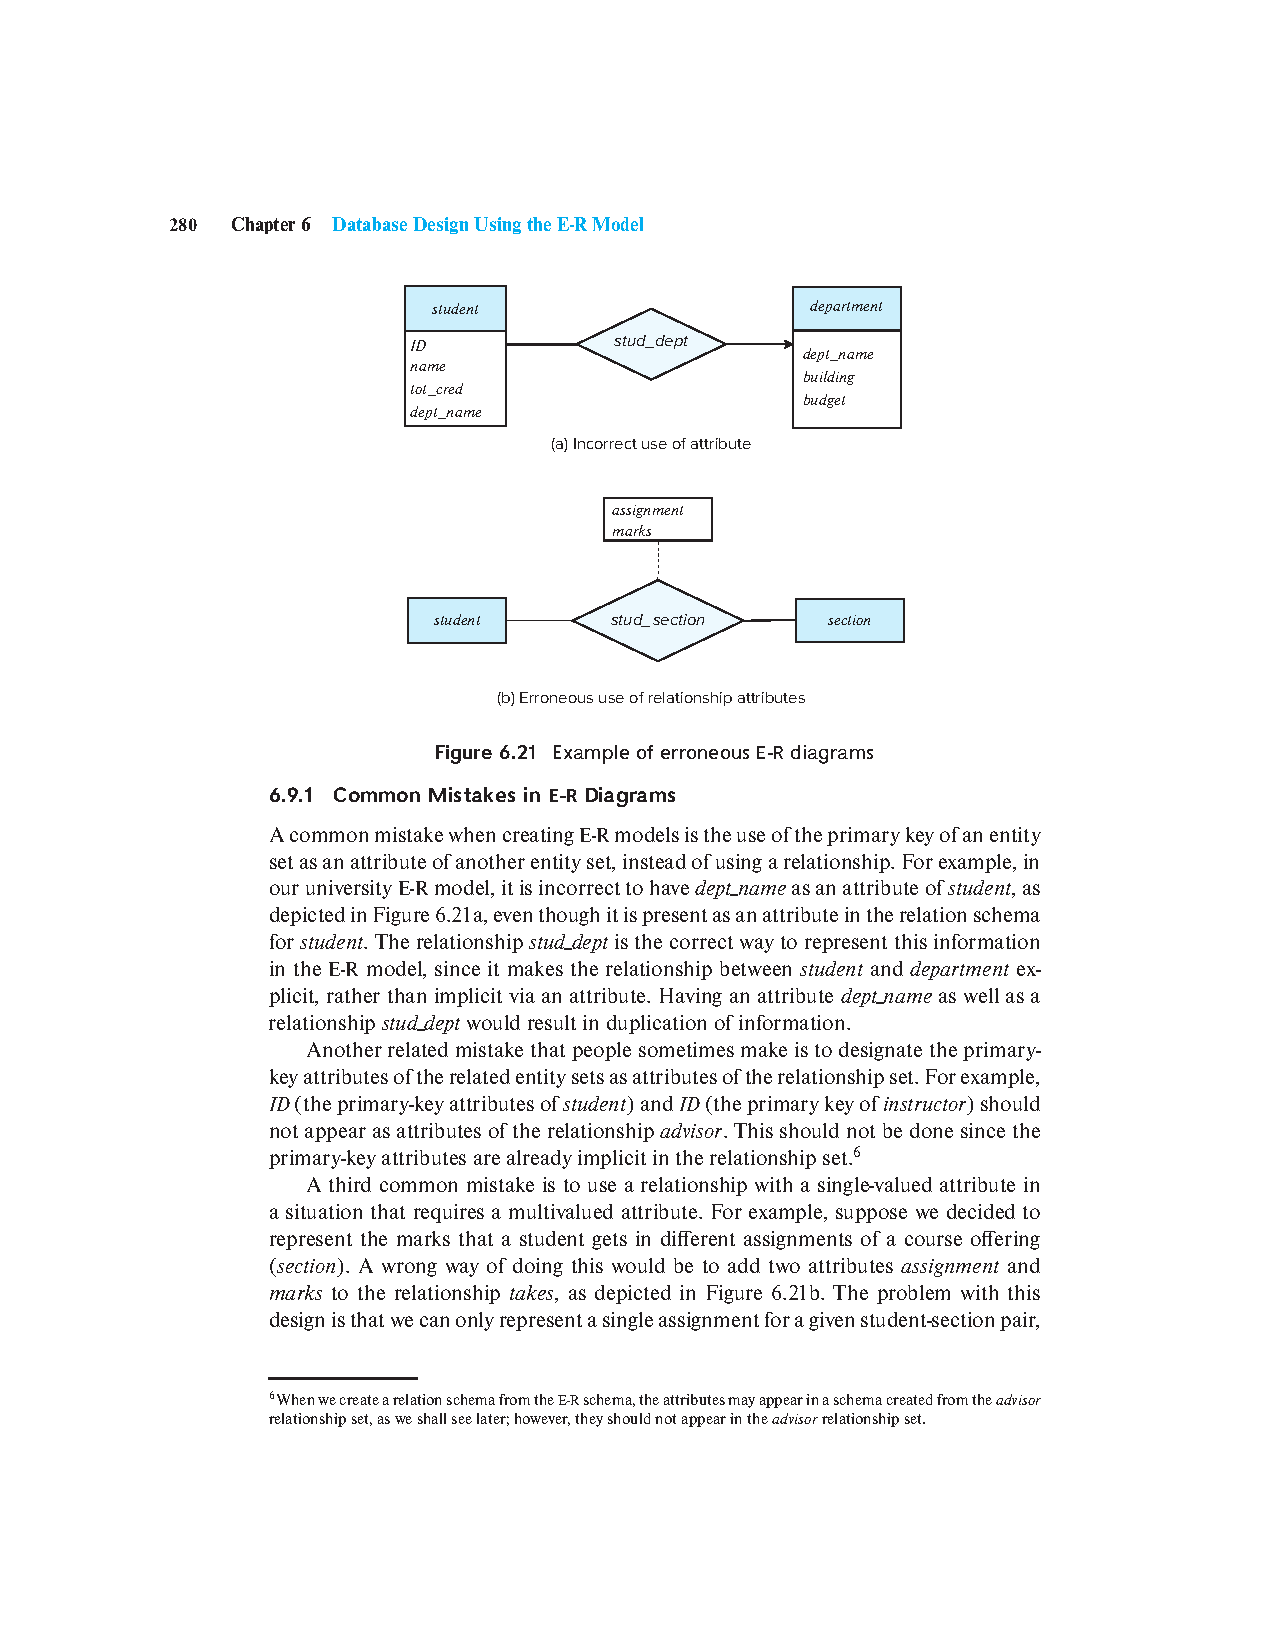
\includegraphics[trim={4cm 16cm 4cm 4cm}, clip, width=\textwidth]{figures/incorrect_use}
\end{frame}

\begin{frame}{Common Mistakes in E-R Diagrams (Cont.)}
    \centering
    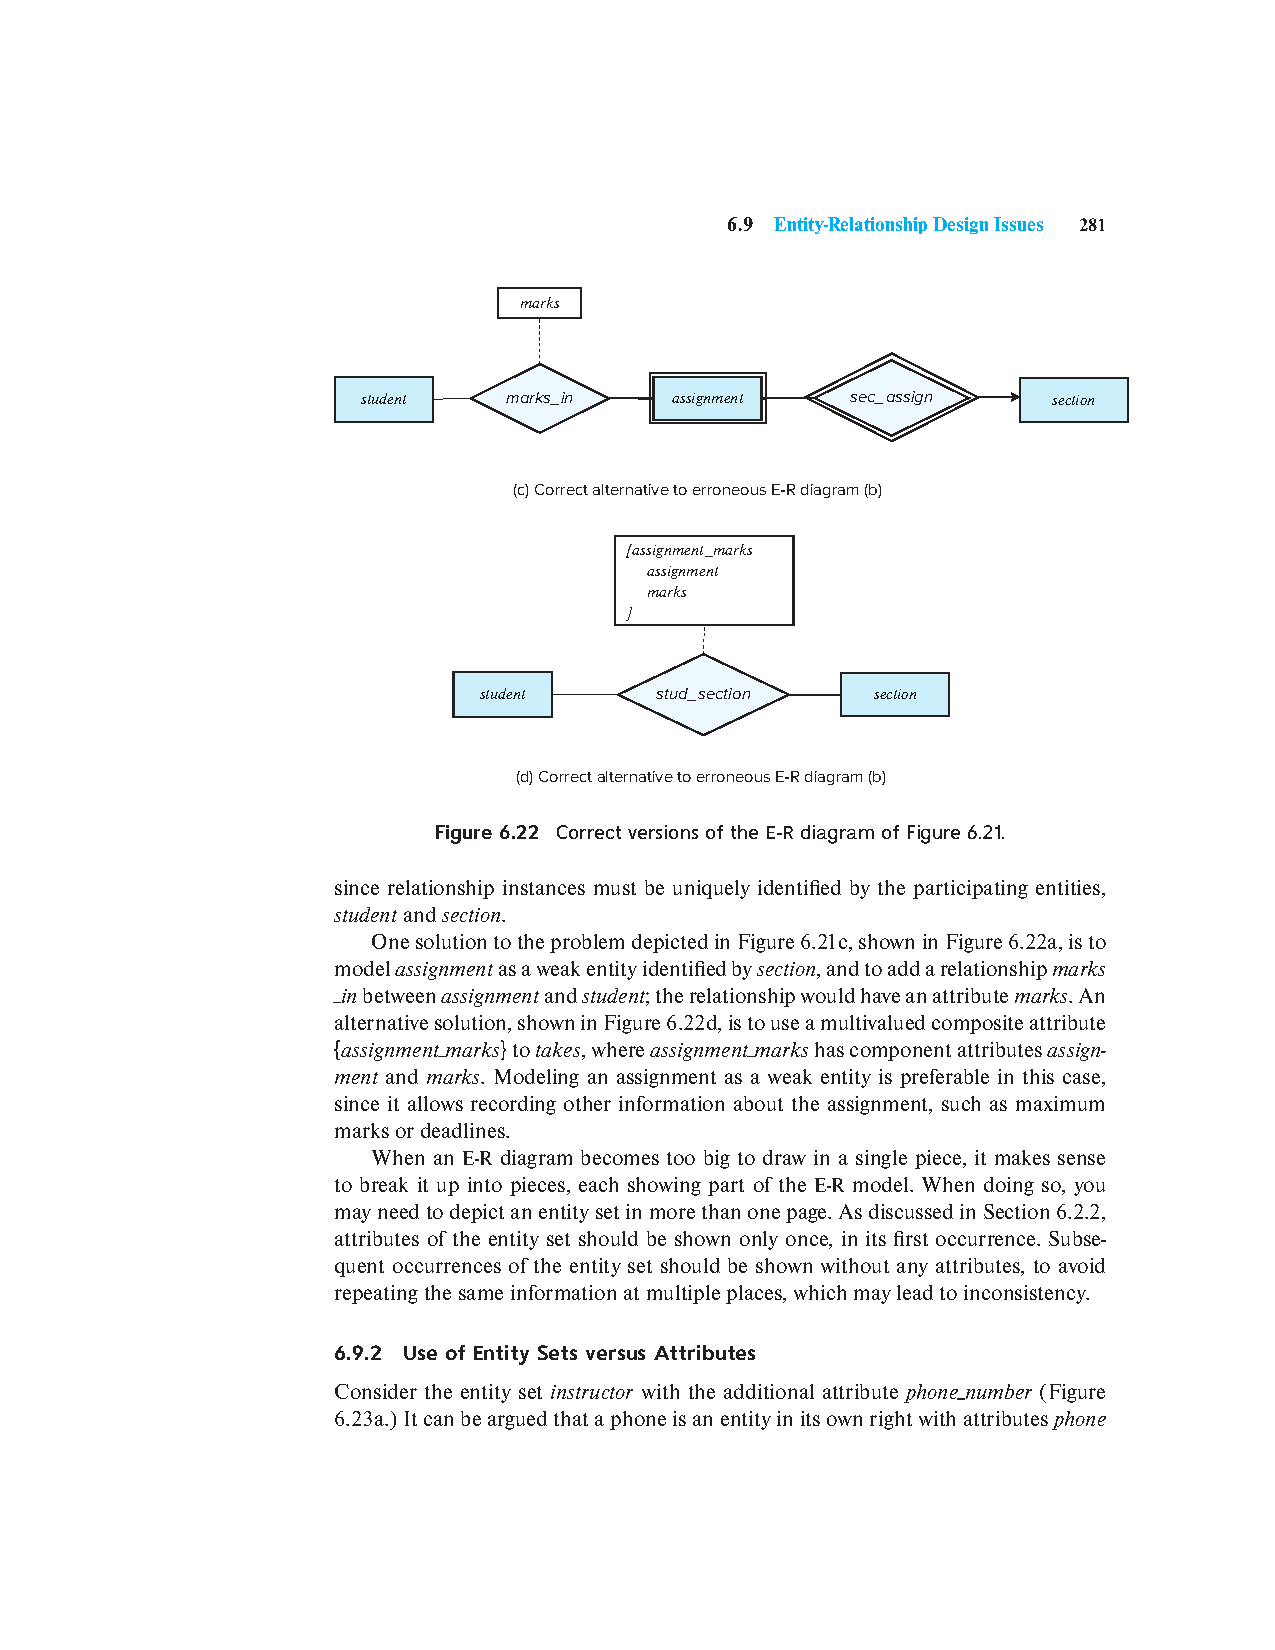
\includegraphics[trim={5.5cm 14cm 2.4cm 4.5cm}, clip, width=\textwidth]{figures/incorrect_use2}
\end{frame}

\begin{frame}{Entities vs. Attributes}
    \begin{itemize}
        \item Use of entity sets vs. attributes:
        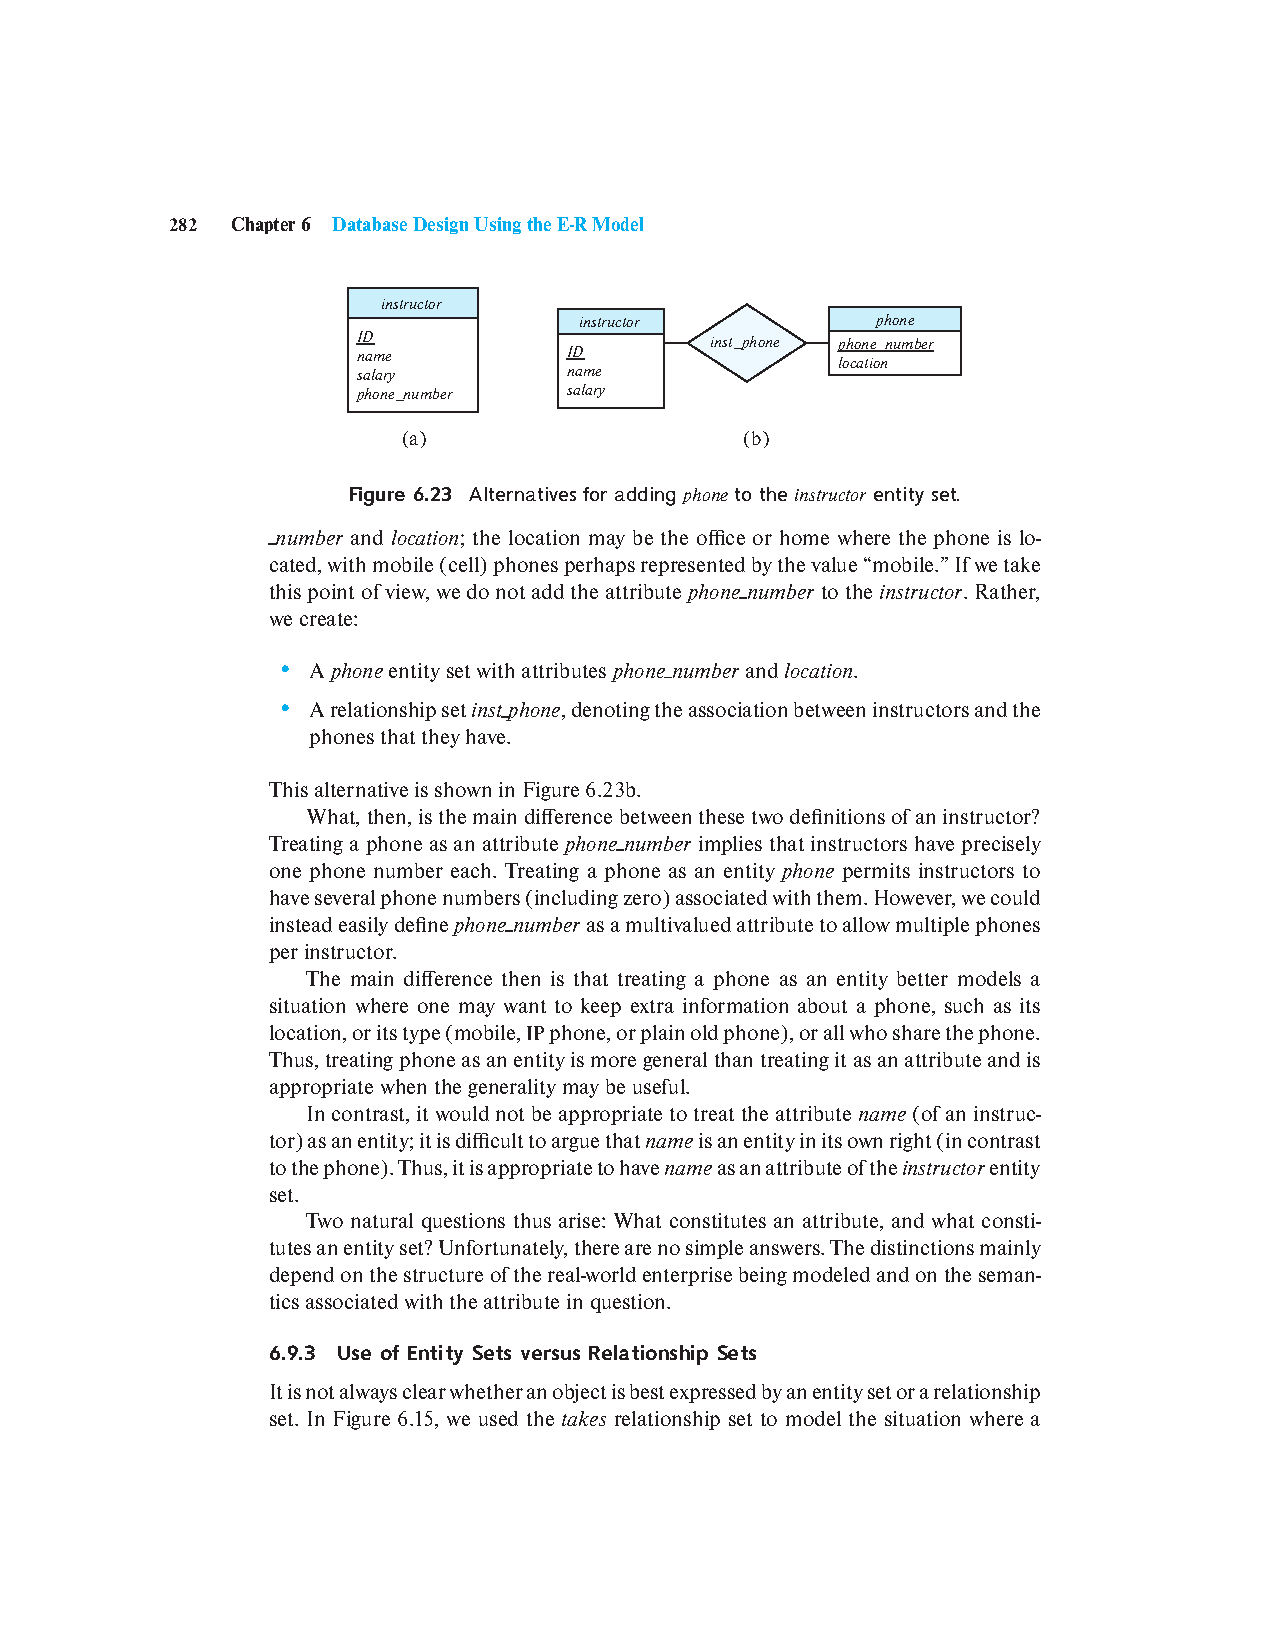
\includegraphics[trim={5cm 20.30cm 4cm 4.75cm}, clip, width=\textwidth]{figures/phones}
        \item Use of phone as an entity allows extra information about phone numbers (plus multiple phone numbers).
    \end{itemize}
\end{frame}

\begin{frame}{Entities vs. Relationship sets}
    \begin{itemize}
        \item \textbf{Use of entity sets vs. relationship sets:}\\
        Possible guideline is to designate a relationship set to describe an action that occurs between entities.
        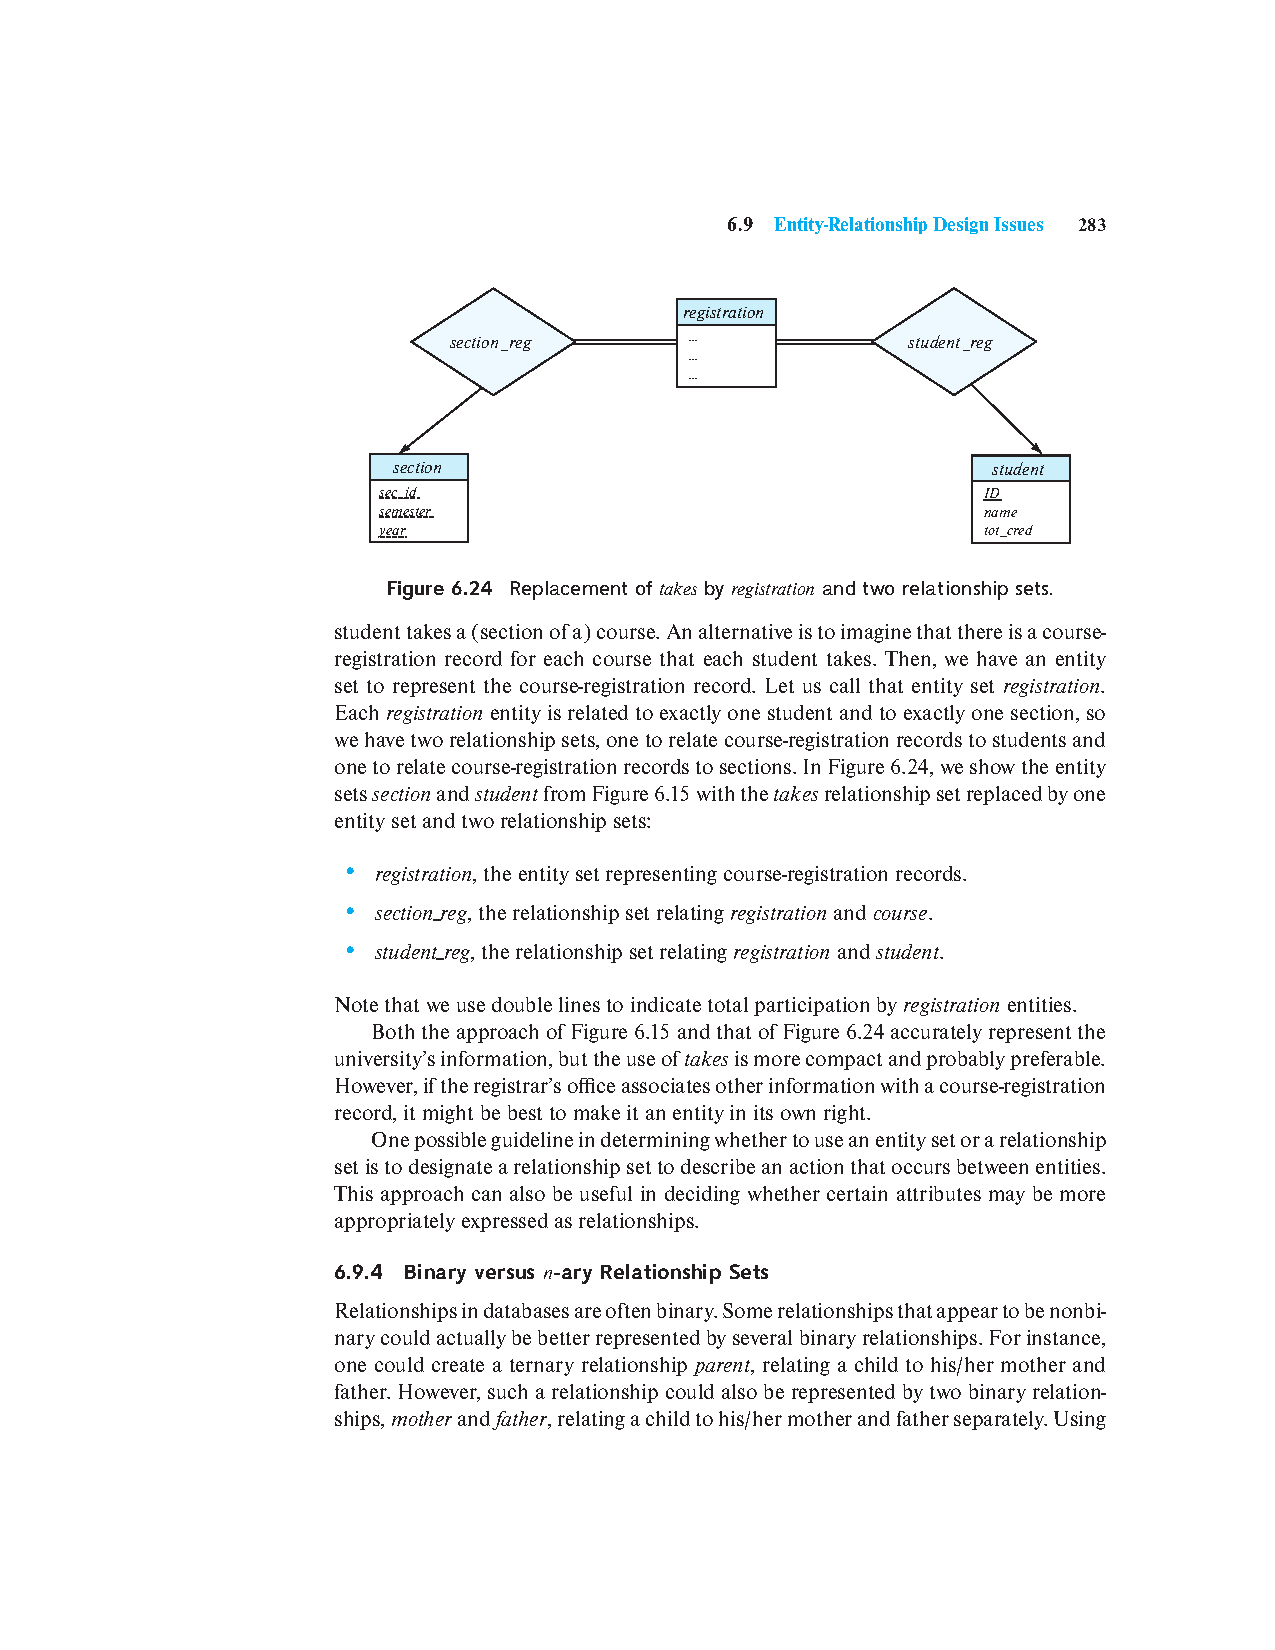
\includegraphics[trim={5cm 18.5cm 0cm 4cm}, clip, width=\textwidth]{figures/registration}
        \item \textbf{Placement of relationship attributes:}\\
        For example, attribute date as attribute of advisor or as attribute of student.
    \end{itemize}
\end{frame}

\begin{frame}{Binary Vs. Non-Binary Relationships}
    \begin{itemize}
        \item Although it is possible to replace any non-binary (n-ary, for $n > 2$) relationship set by a number of distinct binary relationship sets, a n-aryrelationship set shows more clearly that several entities participate in a single relationship.
        \item Some relationships that appear to be non-binary may be better represented using binary relationships:
        \begin{itemize}
            \item For example, a ternary relationship parents, relating a child to his/her father and mother, is best replaced by two binary relationships, father and mother:
            \begin{itemize}
                \item Using two binary relationships allows partial information (e.g., only mother being known).
            \end{itemize}
            \item But there are some relationships that are naturally non-binary.  Example: \texttt{proj\_guide}.
        \end{itemize}
    \end{itemize}
\end{frame}

\begin{frame}{Converting Non-Binary Relationships to Binary Form}
    In general, any non-binary relationship can be represented using binary relationships by creating an artificial entity set:
    \begin{itemize}
        \item Replace R between entity sets A, B and C by an entity set E, and three relationship sets:
        \begin{enumerate}
            \item $R_A$, a many-to-one relationship set from E to A.
            \item $R_B$, a many-to-one relationship set from E to B.
            \item $R_C$, a many-to-one relationship set from E to C.
        \end{enumerate}
    \end{itemize}
    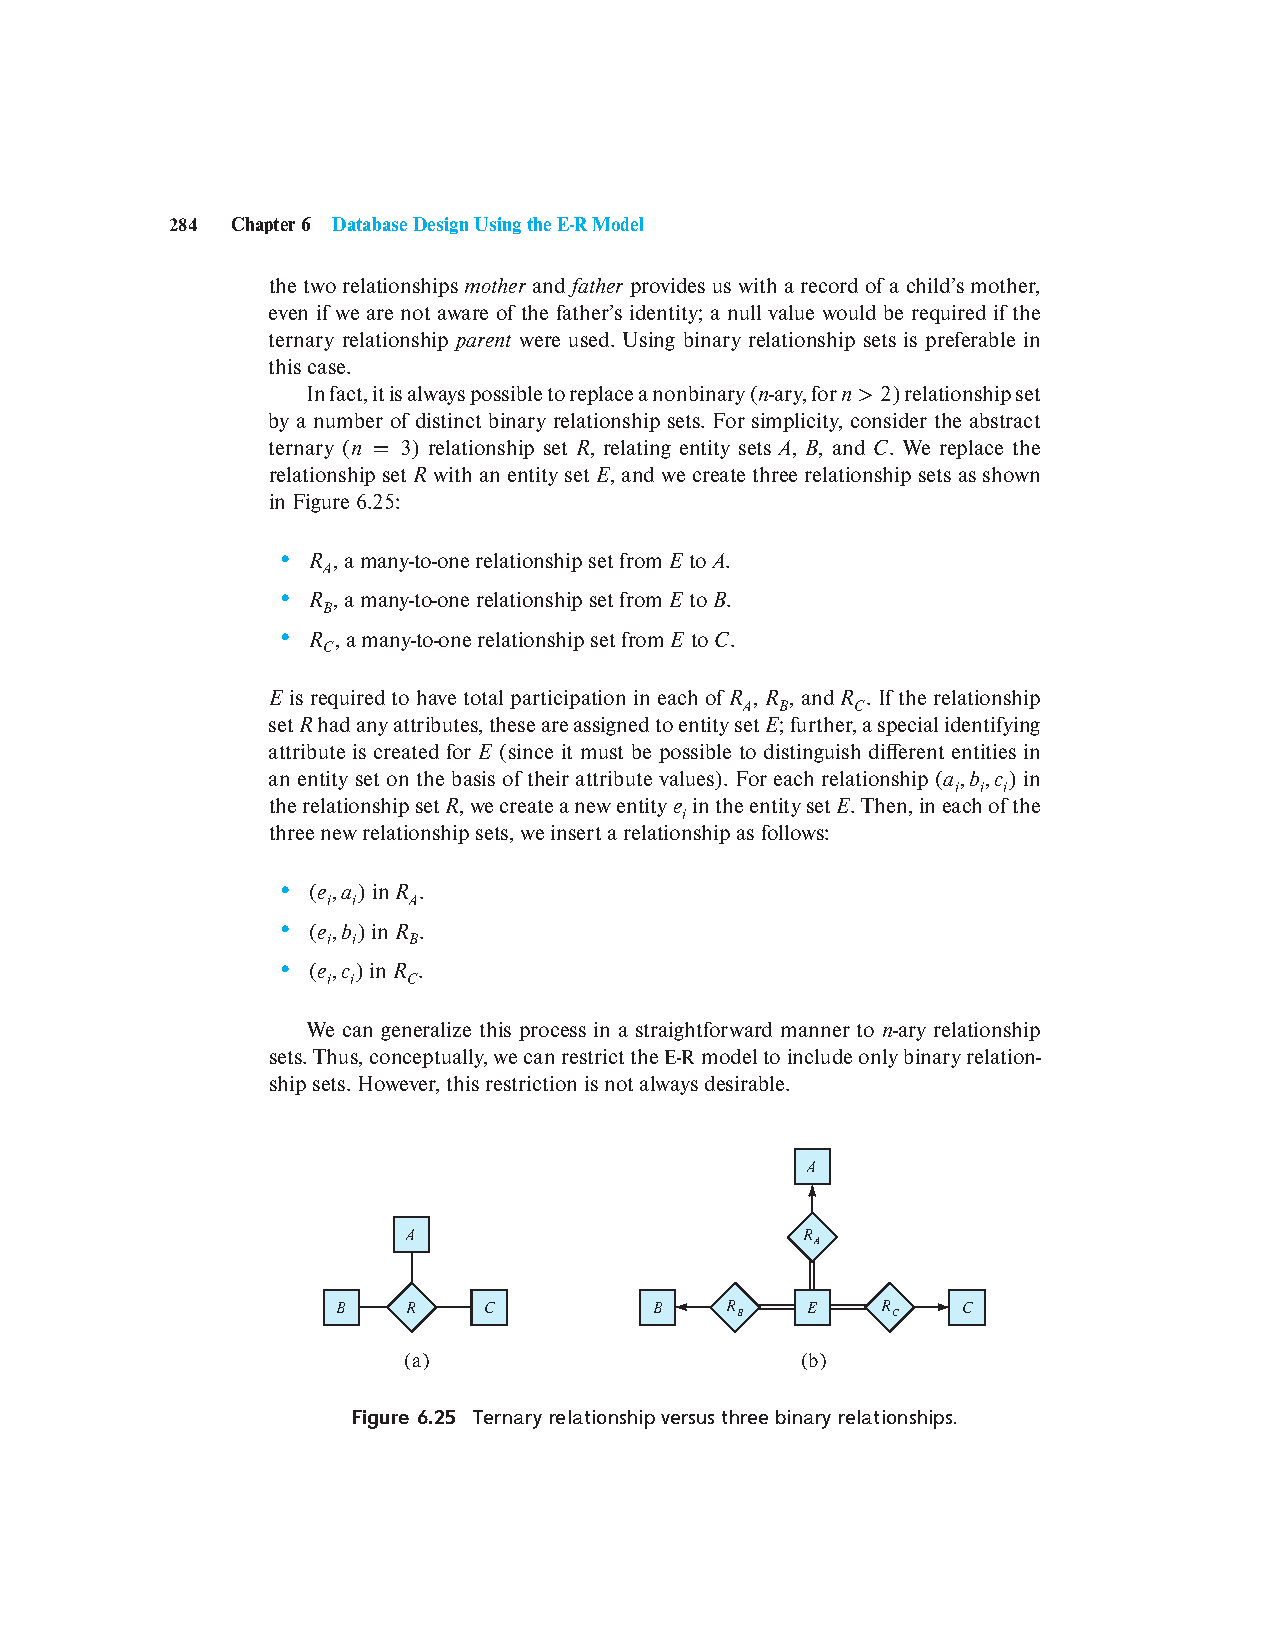
\includegraphics[trim={5cm 4.5cm 4.75cm 19cm}, clip, width=\textwidth]{figures/ternary}
\end{frame}

\begin{frame}{E-R Design Decisions}
    \begin{itemize}
        \item The use of an attribute or entity set to represent an object.
        \item Whether a real-world concept is best expressed by an entity set or a relationship set.
        \item The use of a ternary relationship versus a pair of binary relationships.
        \item The use of a strong or weak entity set.
        \item The use of specialization/generalization -- contributes to modularity in the design.
        \item The use of aggregation -- can treat the aggregate entity set as a single unit without concern for the details of its internal structure.
    \end{itemize}
\end{frame}

\begin{frame}{Summary of Symbols Used in E-R Notation}
    \centering
    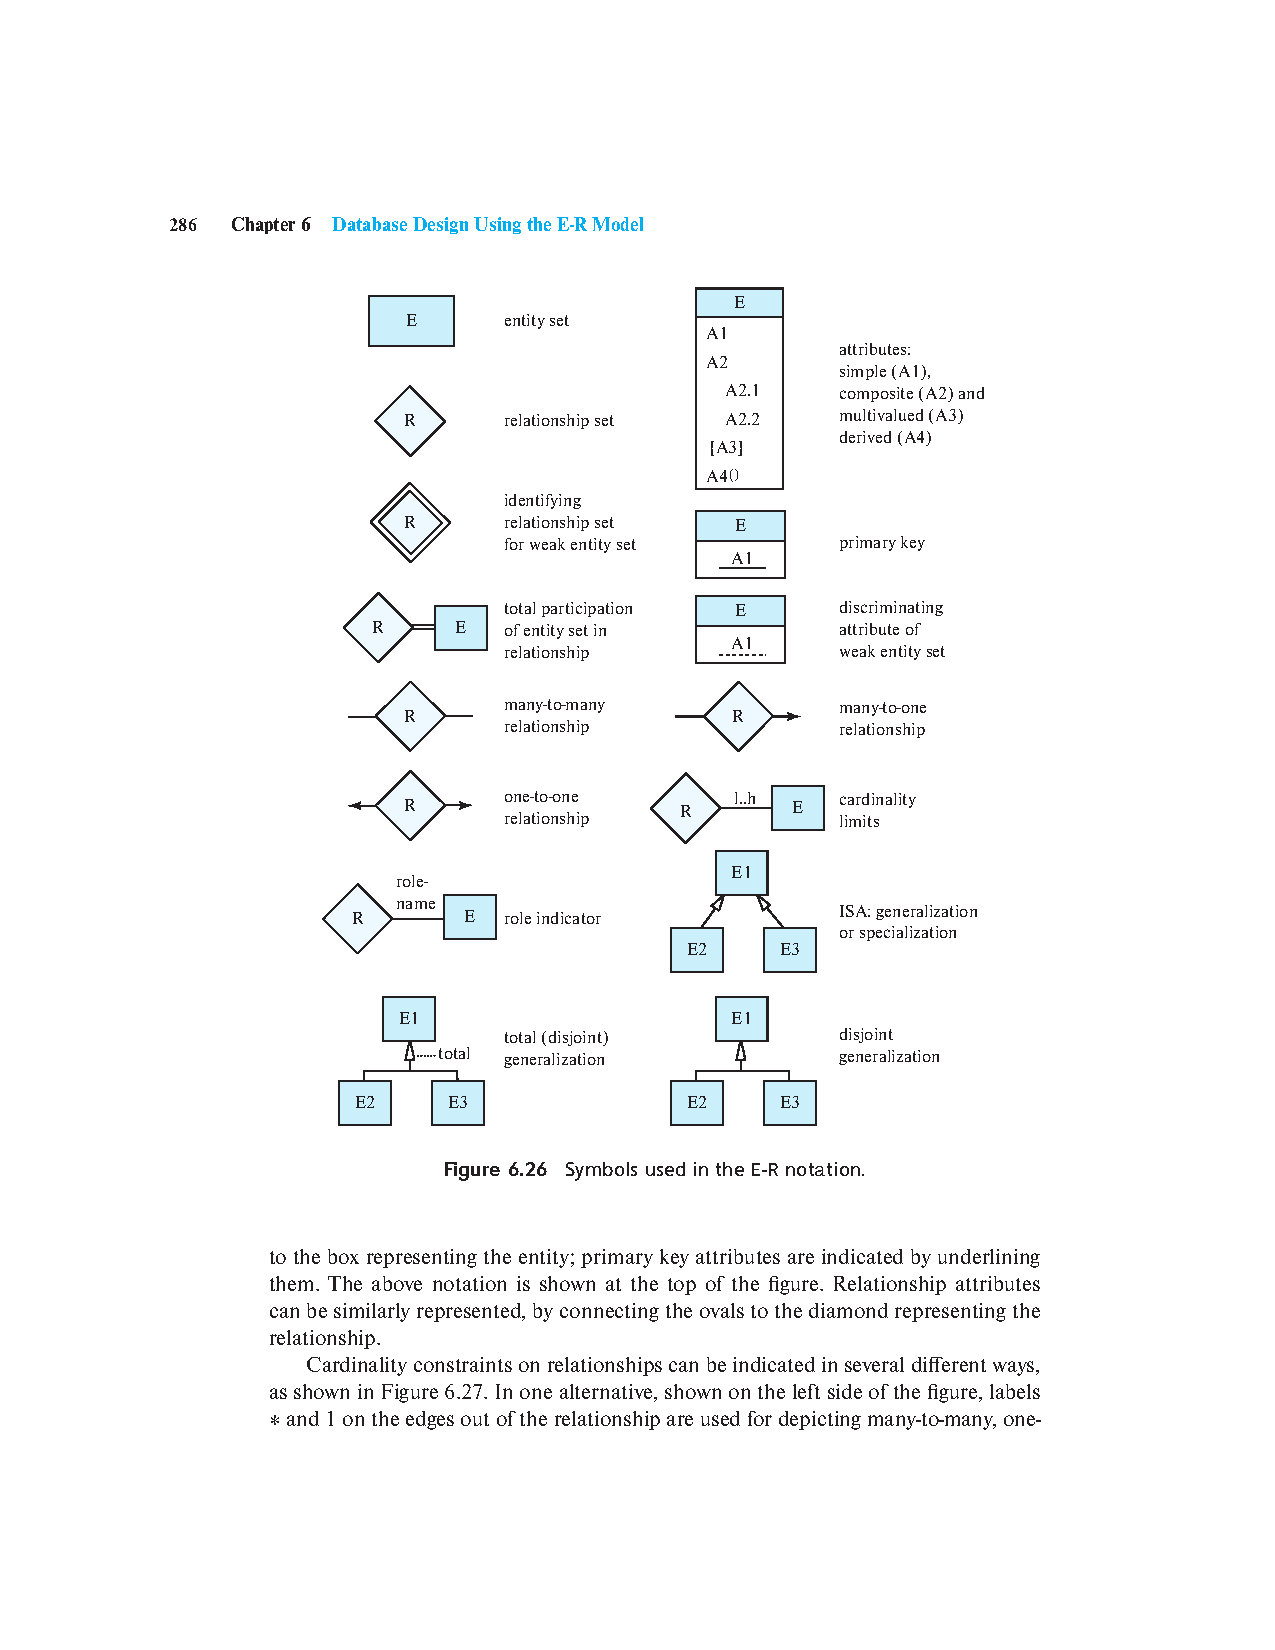
\includegraphics[trim={5.45cm 8.75cm 5.05cm 4.8cm}, clip, width=0.6\textwidth]{figures/symbols}
\end{frame}

\begin{frame}{Alternative ER Notations}
    \centering
    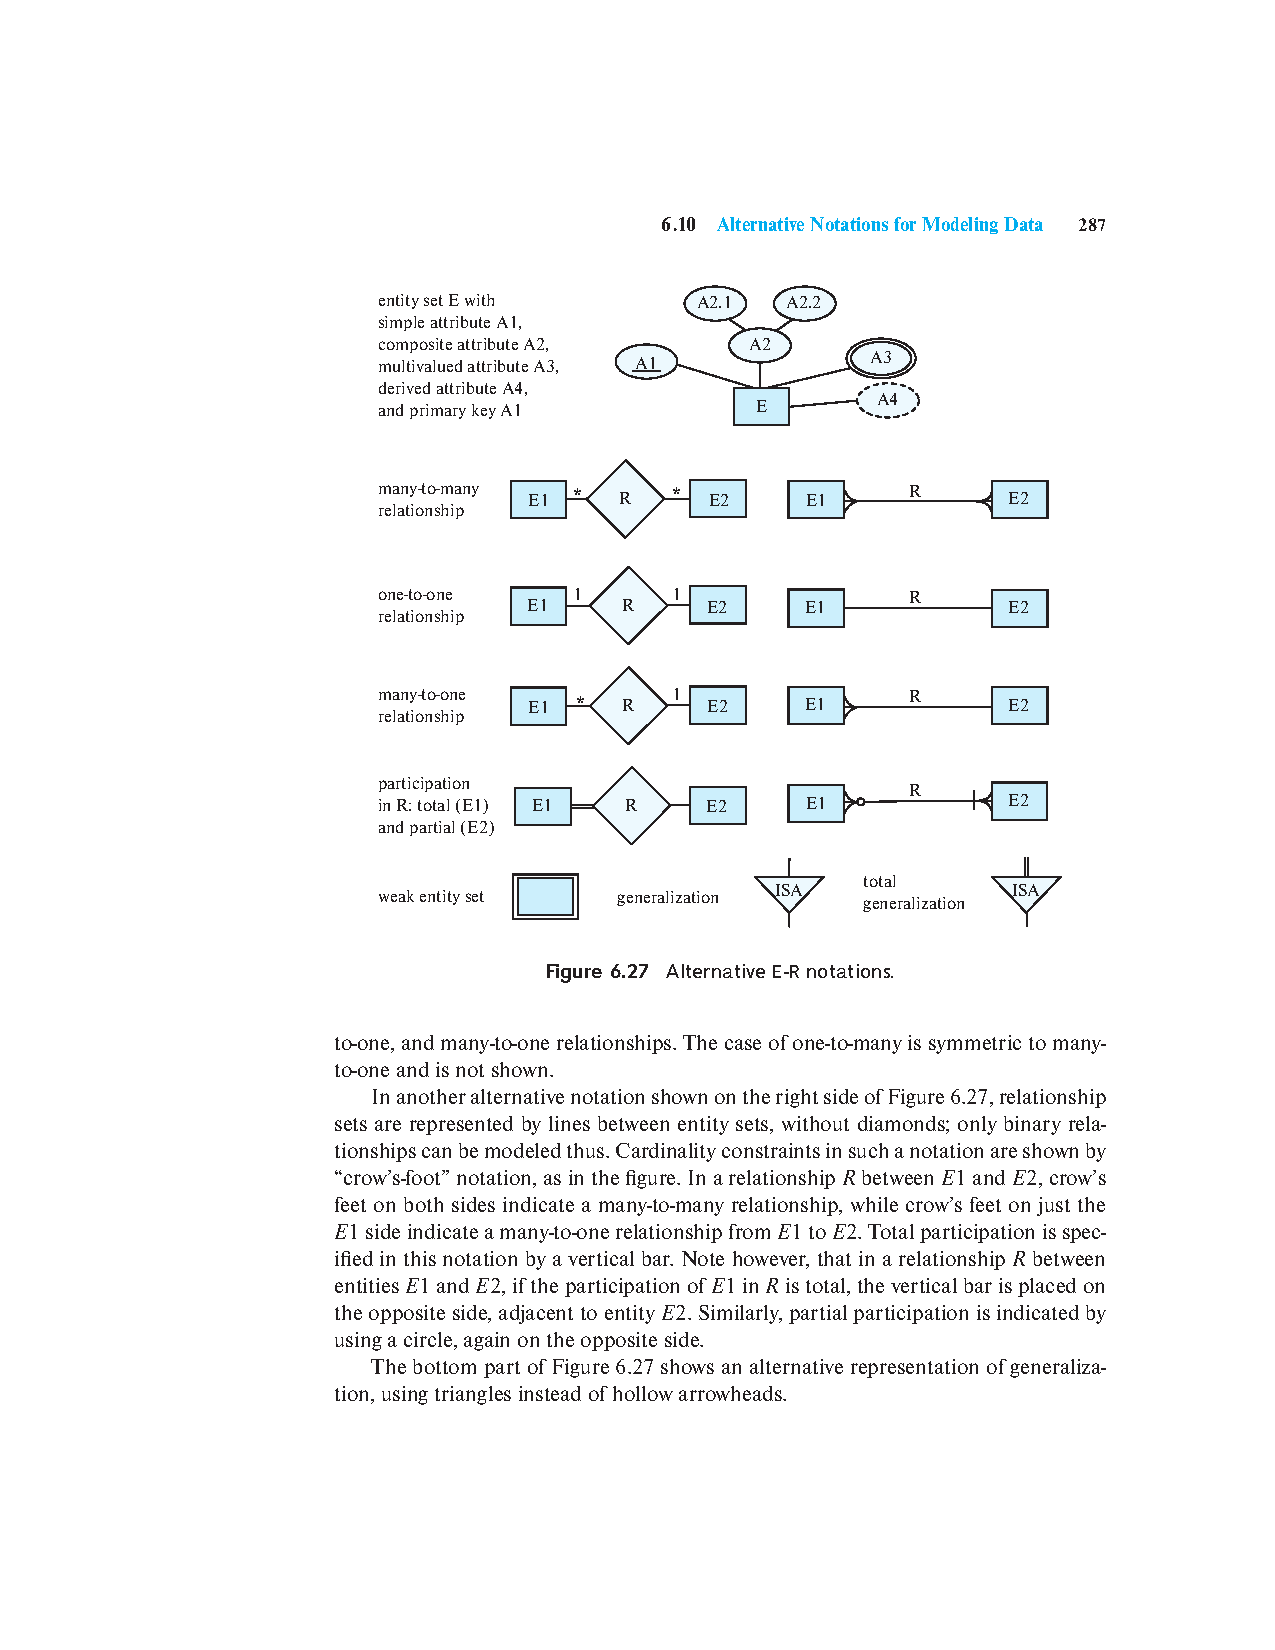
\includegraphics[trim={6.25cm 12cm 3.63cm 4.6cm}, clip, width=0.8\textwidth]{figures/alternative_notations}
\end{frame}

\begin{frame}{UML}
    \begin{itemize}
        \item UML: Unified Modeling Language.
        \item UML has many components to graphically model different aspects of an entire software system.
        \item UML Class Diagrams correspond to E-R Diagram, but some differences.
    \end{itemize}
\end{frame}

\begin{frame}{ER vs. UML Class Diagrams}
    \centering
    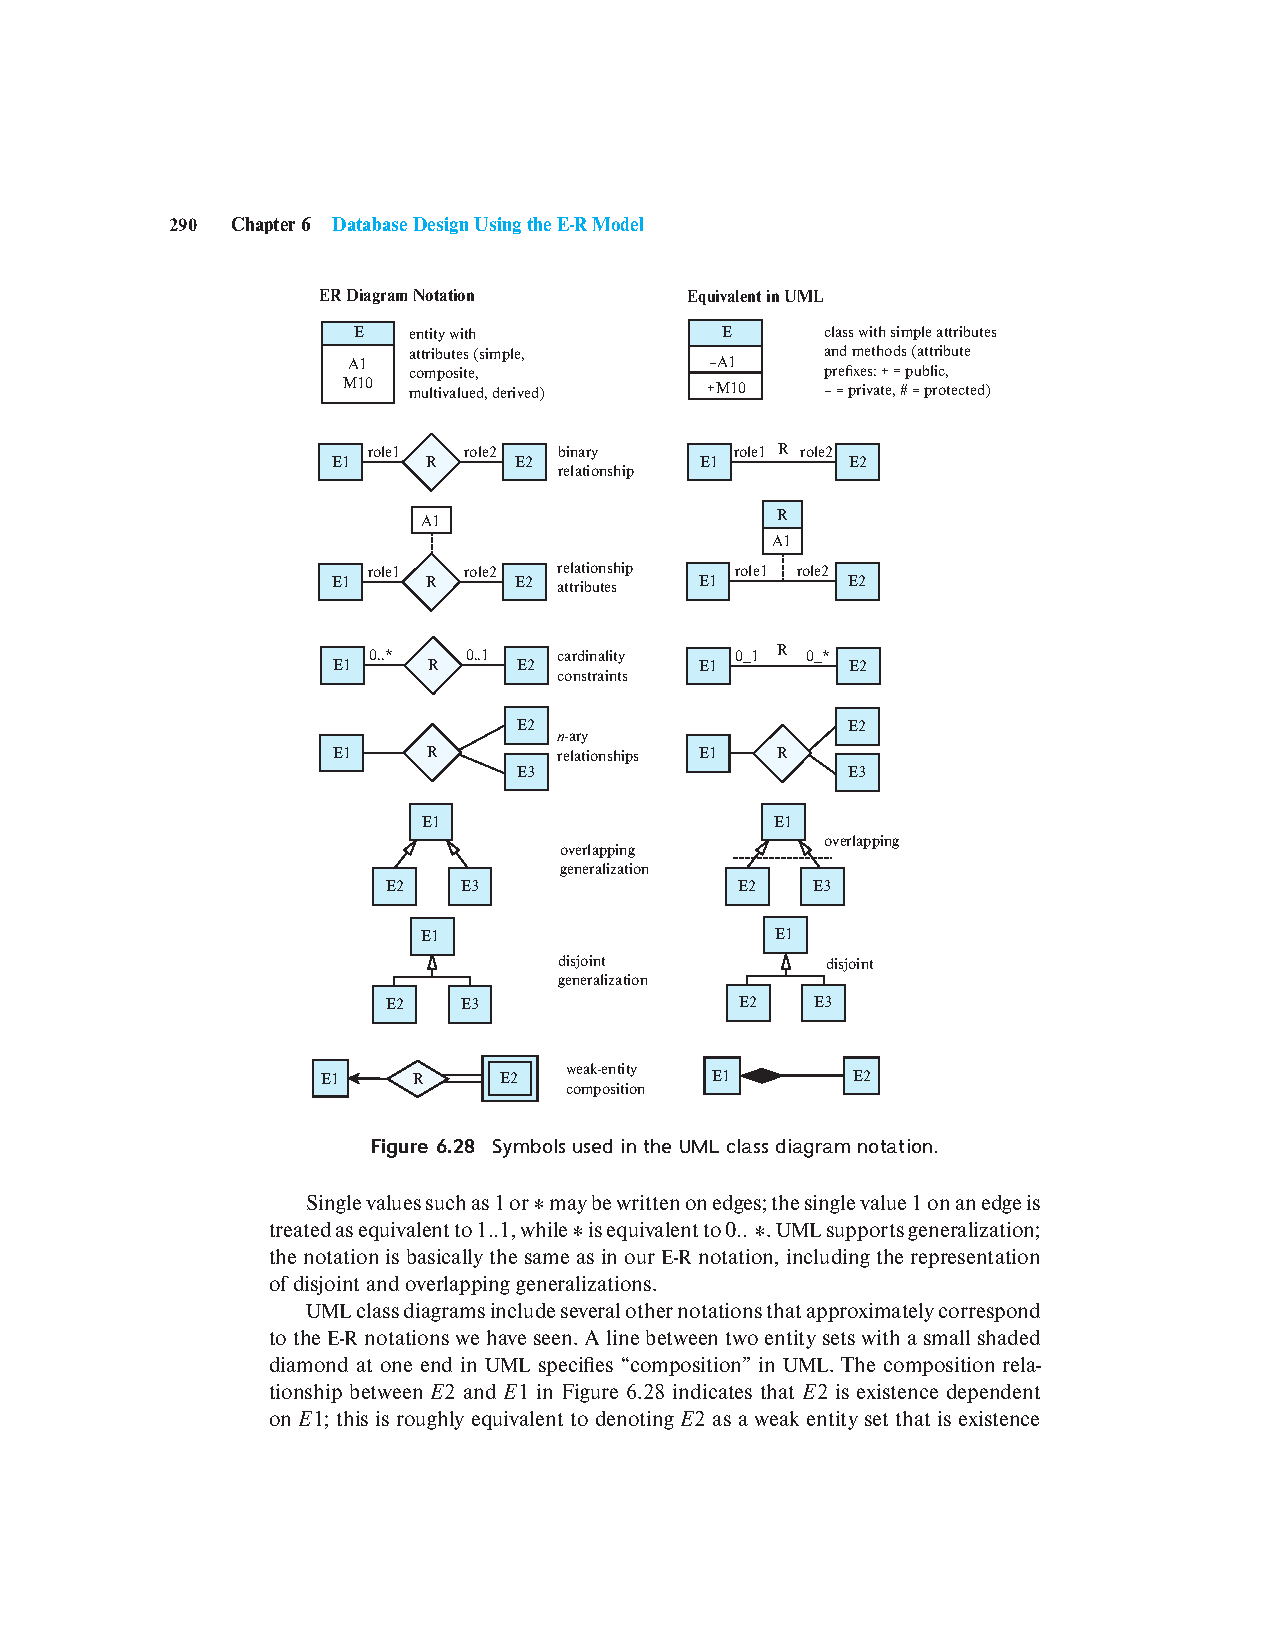
\includegraphics[trim={5cm 9cm 3.63cm 4.6cm}, clip, width=0.7\textwidth]{figures/uml}
\end{frame}

\begin{frame}{UML Class Diagrams (Cont.)}
    \begin{itemize}
        \item Note reversal of position in cardinality constraint depiction.
        \item Generalization can use merged or separate arrows independent of disjoint/overlapping.
        \item Binary relationship sets are represented in UML by just drawing a line connecting the entity sets. The relationship set name is written adjacent to the line.
        \item The role played by an entity set in a relationship set may also be specified by writing the role name on the line, adjacent to the entity set.
        \item The relationship set name may alternatively be written in a box, along with attributes of the relationship set, and the box is connected, using a dotted line, to the line depicting the relationship set.
    \end{itemize}
\end{frame}

\begin{frame}{Other Aspects of Database Design}
    \begin{itemize}
        \item Functional Requirements.
        \item Data Flow, Workflow.
        \item Schema Evolution.
    \end{itemize}
\end{frame}

% \begin{frame}[fragile]{}
%     \begin{minted}
%     [tabsize=4, obeytabs, frame=lines, framesep=2mm, baselinestretch=1.2, bgcolor=LightGray, fontsize=\scriptsize]{sql}
%     \end{minted}
% \end{frame}

\begin{frame}{}
     \centering
     \Huge End of Chapter 6.
\end{frame}

\section*{Takeaways}

% Tim Duncan's Top 5 Fundamental Takeaways of the Today's Class
\begin{frame}{TDT5FTOTTC}
    \centering
    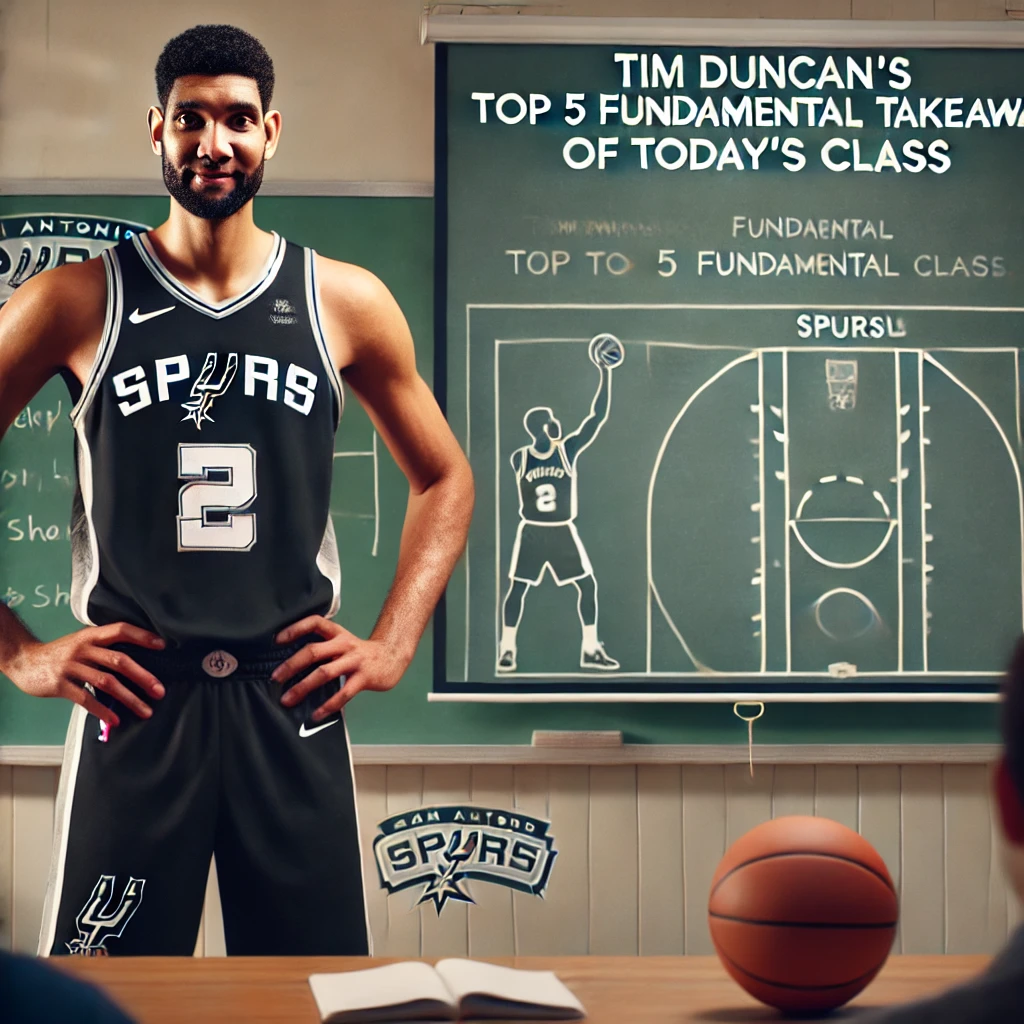
\includegraphics[width=0.75\textwidth]{figures/tim.png}
\end{frame}

\begin{frame}{Top 5 Fundamental Takeaways}
    \small
    \begin{enumerate} \pause
        \item[5] \textbf{Design Phases:} Database design progresses from understanding user requirements to creating a conceptual schema and finally defining logical and physical structures. \pause

        \item[4] \textbf{E-R Model Basics:} The E-R model uses entities, attributes, and relationships to represent and organize data meaningfully. \pause

        \item[3] \textbf{Constraints and Enhancements:} Effective modeling includes specifying cardinality and participation constraints, and using constructs like weak entities, generalization, and aggregation for complex scenarios. \pause

        \item[2] \textbf{Mapping to Schemas:} E-R diagrams are systematically converted into relational schemas by translating entities, attributes, and relationships into tables and foreign keys. \pause

        \item[1] \textbf{Design Choices and Errors:} Good database design requires thoughtful decisions about how to represent real-world concepts and avoiding redundancy or incomplete modeling.
    \end{enumerate}
\end{frame}

\begin{frame}{Database System Concepts}
    \centering
    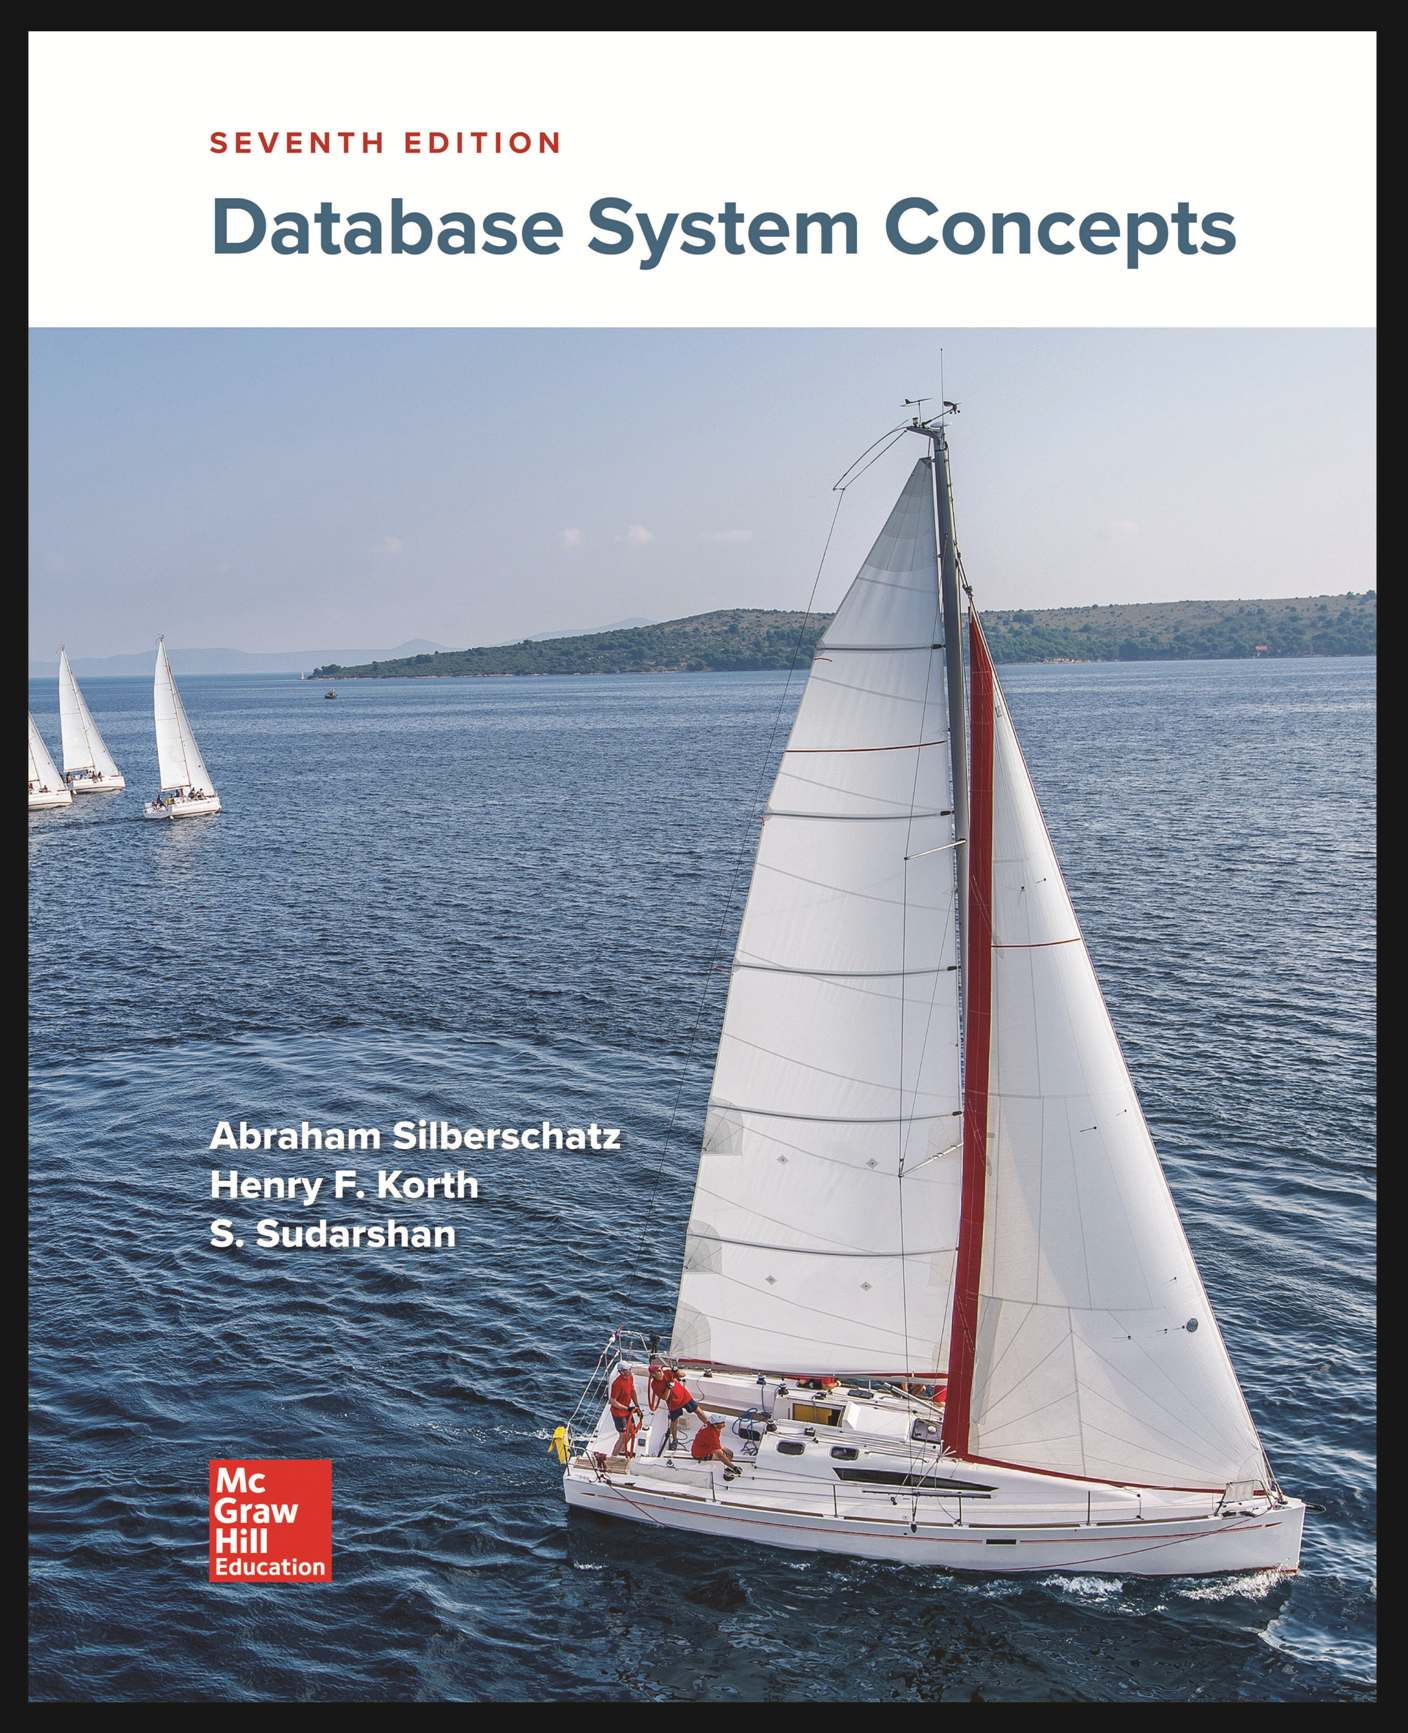
\includegraphics[width=0.5\textwidth]{figures/book_cover.jpg} \\
    \vspace{5mm}
    {
        \tiny
        Content has been extracted from \textit{Database System Concepts}, Seventh Edition, by Silberschatz, Korth and Sudarshan. Mc Graw Hill Education. 2019.\\
        Visit \url{https://db-book.com/}.\\
    }
\end{frame}

\end{document}
